
% Arquivo principal para trabalhos acadêmicos Senai Jaraguá do Sul
% abnTeX2: Modelo de Trabalho Academico em conformidade com 
% ABNT NBR 14724:2011: Informacao e documentacao - Trabalhos academicos -
% Apresentacao

% ------------------------------------------------------------------------
% ------------------------------------------------------------------------

\documentclass[
	12pt,				% tamanho da fonte
	openright,			% capítulos começam em pág ímpar (insere página vazia caso preciso)
	oneside,			% para n imprimir frente e verso
	a4paper,			% tamanho do papel. 
	chapter=TITLE,		% títulos de capítulos convertidos em letras maiúsculas
	%section=TITLE,		% títulos de seções convertidos em letras maiúsculas
	%subsection=TITLE,	% títulos de subseções convertidos em letras maiúsculas
	%subsubsection=TITLE,% títulos de subsubseções convertidos em letras maiúsculas
	% -- opções do pacote babel --
	english,			% idioma adicional para hifenização
	brazil,				% o último idioma é o principal do documento
	]{./Data/udesc}

\usepackage{./Data/udescsty}
\usepackage{color,graphicx}
\usepackage{float}
\usepackage[table,xcdraw]{xcolor}
\usepackage{lscape}


% ---
% Informações de dados para CAPA e FOLHA DE ROSTO
% ---
\titulo{Projeto Integrador}


\autor{Ronei José Roteski, Fernando Marques Candido, Douglas Penna Bastos Blank, Gustavo Giese}
\local{Jaraguá do sul}
\data{2020}
%\fulldata{07 de Agosto de 2013}
\orientador{Proª Msc. Tathiane Duarte do Amarante}
\coorientador{Mario Cleiton}
\instituicao{Faculdade do Estado de Santa Catarina - Senai}
\campus{Senai Jaragua do Sul}
%\tipotrabalho{Mestrado}
%\tipodoc{Dissertação}
\curso{Sistemas para Internet}
%\titulacao{Mestre em Engenharia Elétrica}
%\area{Automação de Sistemas}
%\nivelgrau{Mestrado Acadêmico}
%\preambulo{Dissertação submetida ao Programa de Pós-Graduação em Engenharia Elétrica do Centro de Ciências Tecnológicas da Universidade do Estado de Santa Catarina, para a obtenção do grau de Mestre em Engenharia Elétrica.}
% ---

% ----
% Início do documento
% ----
\begin{document}
% ----------------------------------------------------------
% ELEMENTOS PRÉ-TEXTUAIS
% ----------------------------------------------------------
% Retira espaço extra obsoleto entre as frases.
\frenchspacing 

% \pretextual

% ---
% Capa
% ---
\imprimircapa
% ---

% ---
% Folha de rosto
% (o * indica que haverá a ficha bibliográfica)
% ---
%\imprimirfolhaderosto*
% ---

% ---
% Inserir a ficha bibliografica
% ---

% Isto é um exemplo de Ficha Catalográfica, ou ``Dados internacionais de
% catalogação-na-publicação''. Você pode utilizar este modelo como referência. 
% Porém, provavelmente a biblioteca da sua universidade lhe fornecerá um PDF
% com a ficha catalográfica definitiva após a defesa do trabalho. Quando estiver
% com o documento, salve-o como PDF no diretório do seu projeto e substitua todo
% o conteúdo de implementação deste arquivo pelo comando abaixo:
%
% \begin{fichacatalografica}
%     \includepdf{fig_ficha_catalografica.pdf}
% \end{fichacatalografica}
%\begin{fichacatalografica}
%	\hrule							% Linha horizontal
%	\begin{center}					% Minipage Centralizado
%	\begin{minipage}[c]{12.5cm}		% Largura
	
%	\imprimirautor
	
%	\hspace{0.5cm} \imprimirtitulo  / \imprimirautor. --
%	\imprimirlocal, \imprimirdata-
	
%	\hspace{0.5cm} \pageref{LastPage} p. : il. (algumas color.).\\
	
%	\hspace{0.5cm} \imprimirorientadorRotulo~\imprimirorientador\\
	
%	\hspace{0.5cm}
%	\parbox[t]{\textwidth}{\imprimirtipotrabalho~--~\imprimirinstituicao,
%	\imprimirdata.}\\
	
%	\hspace{0.5cm}

	
%	\end{minipage}
%	\end{center}
%	\hrule
%\end{fichacatalografica}
% ---


% ---
% Inserir errata (Se necessário)
% ---
%\begin{errata}
%Elemento opcional da \citeonline[4.2.1.2]{NBR14724:2011}. Exemplo:
%
%\vspace{\onelineskip}
%
%FERRIGNO, C. R. A. \textbf{Tratamento de neoplasias ósseas apendiculares com
%reimplantação de enxerto ósseo autólogo autoclavado associado ao plasma
%rico em plaquetas}: estudo crítico na cirurgia de preservação de membro em
%cães. 2011. 128 f. Tese (Livre-Docência) - Faculdade de Medicina Veterinária e
%Zootecnia, Universidade de São Paulo, São Paulo, 2011.
%
%\begin{table}[htb]
%\center
%\footnotesize
%\begin{tabular}{|p{1.4cm}|p{1cm}|p{3cm}|p{3cm}|}
%  \hline
%   \textbf{Folha} & \textbf{Linha}  & \textbf{Onde se lê}  & \textbf{Leia-se}  \\
%    \hline
%    1 & 10 & auto-conclavo & autoconclavo\\
%   \hline
%\end{tabular}
%\end{table}
%
%\end{errata}
% ---

% ---
% Inserir folha de aprovação
% ---

% Isto é um exemplo de Folha de aprovação, elemento obrigatório da NBR
% 14724/2011 (seção 4.2.1.3). Você pode utilizar este modelo até a aprovação
% do trabalho. Após isso, substitua todo o conteúdo deste arquivo por uma
% imagem da página assinada pela banca com o comando abaixo:
%
% \includepdf{folhadeaprovacao_final.pdf}
%
%\begin{folhadeaprovacao}

 %   \begin{center}
%    {\ABNTEXchapterfont\bfseries\Large\imprimirtitu%lo}
    
%    \vspace*{\fill}
    
    
%    \vspace*{\fill}
%  	{\ABNTEXchapterfont\bfseries\large\MakeUppercase{\imprimirautor}}
    
%    \vspace*{\fill}
%     \MakeLowercase{\imprimirtipodoc}
        
%    \vspace*{\fill}
%    {\ABNTEXchapterfont\bfseries\Large\imprimirtitulacao}
    
%    \vspace*{\fill}
   
      
%    \vspace*{\fill}
    
   % \normalsize\MakeUppercase{%
  %  Curso de \imprimirnivelgrau \, em %\imprimircurso \, do
 %   centro de ciências tecnológicas da
 %   universidade do estado de santa catarina.}	
	
%	\vspace*{\fill}
%	\begin{minipage}[h!]{0.35\textwidth}
%		\centering
	

%	\imprimirlocal,
%	\par 
%	\imprimirfulldata:
%	\end{minipage}    
  % 	\hfill
%	\begin{minipage}[h!]{0.62\textwidth}
 
 
   %\assinatura{\textbf{Professor} \\ Convidado 4}
%   \end{minipage}  
 %  \end{center}
%\end{folhadeaprovacao}
% ---

% ---
% Dedicatória
% ---
%\begin{dedicatoria}
   %\vspace*{\fill}
   %\centering
   %\noindent
   %\textit{ Agradeço a meus colegas e professores %por me ajudarem no meu caminho acadêmico.} %\vspace*{\fill}
%\end{dedicatoria}
% ---

% ---
% Agradecimentos
% ---
%\begin{agradecimentos}
%Gostaria de agradecer...
%
%A todos que me ajudaram em minhas dificuldades.
%\end{agradecimentos}
% ---

% ---
% Epígrafe
% ---
%\begin{epigrafe}
    %\vspace*{\fill}
	%\begin{flushright}
		%\textit{O esforço traz grandes frutos , %mais também suas responsabilidades.}
%	\end{flushright}
%\end{epigrafe}
% ---

% ---
% RESUMOS
% ---

% resumo em português
\begin{resumo}
	O objetivo deste trabalho e produzir um software para melhorar a logística de ordens de manutenção que hoje em dia e feito por meio manual trazendo inúmeros problemas e prejuízos para  a empresa. Neste documento irá ser descrito e apresentado o problema , esclarecendo os objetivos e mostrando uma solução.

 \vspace{\onelineskip}
    
 \noindent
 
\end{resumo}

% resumo em inglês
\begin{resumo}[Abstract]
 \begin{otherlanguage*}{english}
	The purpose of this work is to produce a software to improve the logistics of maintenance orders that today is done by manual means bringing numerous problems and damages to the company. In this document the problem will be described and presented, clarifying the objectives and showing a solution.

   \vspace{\onelineskip}
 
   \noindent 

 \end{otherlanguage*}
\end{resumo}

% ---
% inserir lista de ilustrações
% ---
\pdfbookmark[0]{\listfigurename}{lof}
\listoffigures*
\cleardoublepage
% ---

% ---
% inserir lista de tabelas
% ---
\pdfbookmark[0]{\listtablename}{lot}

\cleardoublepage
% ---

% ---
% inserir lista de abreviaturas e siglas
% ---
%\begin{siglas}
%  \item[OS]       ordem serviço

%\end{siglas}
% ---

% ---
% inserir lista de símbolos
% ---


% ---
% inserir o sumario
% ---
\pdfbookmark[0]{\contentsname}{toc}

\tableofcontents*
\cleardoublepage
% ---

\textual
% ---

% ----------------------------------------------------------
% ELEMENTOS TEXTUAIS
% ----------------------------------------------------------

\chapter{Introdução}

{\color{red}
	
DOUGLAS BLANK
	
Para o desenvolvimento de projetos ligados diretamente a industria, a Faculdade Senai de Jaraguá do sul tem adotado o método de \textit{Projetos Integradores}, que é uma estratégia de ensino–aprendizagem cujo objetivo é proporcionar a interdisciplinaridade entre todos os temas/assuntos/bases abordados durante o curso de operador de computador.

O processo de realização do \textit{Projeto Integrador} fornece subsídios para a avaliação das competências relacionadas ao perfil profissional do operador de computador e seu objetivo maior é “articular teoria e prática” mediante o contato do aluno com diversos contextos do mundo do trabalho com as industrias da região \cite{magalhaes2019uso}.  

A empresa parceira para o desenvolvimento do \textit{Projeto Integrador} da foi a Duas Rodas Alimentos,  que  possui sua matriz na cidade de  em Jaraguá do Sul, Santa Catarina  \footnote{\url{ https://www.duasrodas.com/}}.  Ela utiliza como ERP (Enterprise Resource Planning) o SAP (Second Audio Program), que trata-se de um software de gestão de empresas.
Com os avanços tecnológicos acontecendo cada vez rápido, torna-se ainda mais essenciais que as empresas se adaptem as tendências do mercado, permitindo maior eficiência nos processos e controle das informações.

}
% 


\section{Tema}
% ---
%Este projeto envolve a digitalização dos processos de uma empresa no setor industrial, a geração de ordens de manutenção, o controle de estoque e desenvolvimento de aplicativo para celulares. O projeto aborda um sistema de gestão de manutenção, que possa gerir as atividades realizadas pelos manutentores, com um abordagem voltada para aumentar a eficiência das atividades realizadas. 
Este projeto está focado na digitalização dos processos de manutenção no setor industrial da empresa em questão, geração de ordens de serviço, consulta de estoque e desenvolvimento de um aplicativo para smartphones. O projeto aborda um sistema de gestão de manutenção, que possa gerir as atividades realizadas pelos manutentores, com foco em aumentar a eficiência das atividades realizadas.
{\color{red} Melhorar o Tema de vcs, pelo menos umas 10 linhas bem detalhadas}
% ---
\section{Objetivo do Projeto}
% ---
%Este projeto tem como objetivo o desenvolvimento de um sistema que digitalize o processo de geração de ordens de manutenção bem como a manipulação desses dados para um melhor gerenciamento. Outra necessidade é com relação a integração do SAP com o Smart Solution para agilizar o processo de retorno das ordens de serviço, além disso nosso projeto tem por finalidade melhorar o gerenciamento dos dados, relatórios, consulta, controle de estoque, histórico e gráficos.
Este projeto tem como objetivo o desenvolvimento de um sistema que digitalize o processo de geração de ordens de manutenção bem como a manipulação desses dados para um melhor gerenciamento. Outra necessidade é com relação a integração do SAP com o \textit{Smart Solution} para agilizar o processo de retorno das ordens de serviço, além disso o projeto tem por finalidade melhorar o gerenciamento dos dados, relatórios, consulta, controle de estoque, histórico e gráficos e por consequência, reduzir o consumo de papel.

{\color{red} ok}
% ---
\section{Delimitação do Problema}
% ---

A base do projeto em questão, tem como foco a digitalização da geração e controle de ordens de serviço, para que o sistema se adeque as necessidades da empresa Duas Rodas, o sistema contem uma aplicação Web para que os funcionários com permissão de acesso possam trabalhar, também foi desenvolvido uma aplicação mobile, para tornar mais dinâmico o trabalho dos manutentores e dessa forma analisar as ordens em que foi executado.
Com a análise dos requisitos iniciais da empresa, também foi desenvolvido um sistema de estoque para o almoxarifado, visando facilitar o controle e requisição de peças conforme a demanda. Por fim, o sistema foi estruturado para ser compatível com o sistema SAP, atualmente em execução na empresa.

{\color{red} Como o projeto ja foi desenvolvido boa parte dele cuidar com os verbos SERÁ desenvolvido  por FOI desenvolvido, pois vcs ja executaram}


\section{Método de Trabalho}
%O projeto será desenvolvido em equipes de 3 a 4 pessoas, com funções específicas para a realização das diversas tarefas. Para o desenvolvimento do projeto, serão utilizados os conceitos de orientação a objetos, além de ser necessário outros conhecimentos técnicos, como o desenvolvimento para aplicativos mobile através de Ionic e Node.Js, sistemas Web com o framework Angular. O projeto será desenvolvido ao longo de cada semestre em diversos entregáveis, estes terão datas pré-definidas, que deveram ser atendidas pelos membros da equipe.
O projeto foi desenvolvido em equipe, com funções específicas para a realização das diversas tarefas. Para o desenvolvimento do projeto, foram utilizados os conceitos de orientação a objetos, além de ser necessário outros conhecimentos técnicos, como o desenvolvimento para aplicativos mobile através de Ionic e Node.js, sistemas Web com framework VueJs. O projeto foi desenvolvido ao longo de cada semestre em diversos entregáveis, com datas pré-definidas que deveram ser atendidas pelos membros da equipe.
{\color{red} Cuidar com os verbos, melhorar a escrita, e onde vcs chamaram as ferramantas utilizadas, linkar  o repositório de onde baixar, site etc.}

% ---
\section{Organização do Trabalho}
%Este trabalho está dividido em 3 seções onde a seção 1 fala sobre o problema principal, os objetivos do projeto, delimitações do problema, a seção 2 descreve nossa solução para o problema, ferramentas utilizadas e por fim as considerações finais e futuros trabalhos.
Este trabalho está dividido em  3 seções onde a seção 1 trata  dos problemas principais, os objetivos do projeto, delimitações do problema, a seção 2 descreve a solução para o problema, ferramentas utilizadas e por fim as considerações finais e futuros trabalhos.

{\color{red} Vcs tem quantas seções no projeto??? descrever as reais}
\chapter{Pesquisa de Anterioridade}

Fernando Marques Candido

Com o desenvolvimento do presente trabalho, ficou visível que muitas das funcionalidades presentes no sistema, já existem. Há vários sistemas de ordens de serviço e gestão de manutenção atualmente no mercado, a seguir será elencado alguns dos destaques no mercado atualmente.

O sistema da \textit{Auvo} é um sistema de gestão de manutenção, com a capacidade de geração de ordens de manutenção, controle das ordens, relatórios de execução, porém diferente do
projeto apresentado neste documento. O sistema do Auvo é um pouco mais abrangente,
Gestão de orçamentos e cálculo de reembolso de despesas.\cite{Auvo2019}

Outro sistema que também destaca-se, é o \textit{Umov} 
, que permite a geração de ordens de serviço,
os diferenciais deste sistema são o sistema de Geolocalização, Checklists de atividades \cite{umov2019}.

O sistema \textit{Smart Solution}, diferente dos apresentados anteriormente por ser mais específico para as
necessidades da empresa Duas Rodas, assim com design personalizado, desempenho melhor em seus processos.


\chapter{Descrição do Sistema }

DOUGLAS BLANK

Este capítulo tem como objetivo descrever o planejamento dos requisitos  do sistema, o escopo e as principais funções. A descrição geral do sistema deve abrange os itens a seguir: descrição do problema que o software vai resolver, seus envolvidos e suas características para implementação de cada função na solução.



\section{Descrição do Problema}
% ---
 {\color{red} melhorar essa introdução que eu adicionei.......
 O  Sistema foi desenvolvido para sanar as dificuldades que a empresa tem com relação as ordens de manutenção serem exclusivamente de maneira manual, buscando de forma prática e objetiva deixando as informações necessárias para a execução dos trabalho mais rápidas e eficientes.}

Sendo assim, o sistema desenvolvido tem como objetivo resolver principalmente os problemas descritos a seguir:
%O desenvolvimento deste sistema, tem como objetivo resolver principalmente os problemas a seguir:

\begin{itemize}
	\item Fluxo lento nos processos de manutenção industrial na empresa.
	\item Falta de automação.
	\item Logística complicada.
	\item Falta de Controle das informações.
	\item Dificuldade em armazenar informações.
	\item Utilização excessiva de papel.
	%\item

\end{itemize}

{\color{red} Melhorar essa descrição} O software \textit{Smart Solution} tem  como diferencial tornar possível, melhorando a eficiência os itens a seguir:

\begin{itemize}

	\item Transformar o processo de manutenção em um processo digital de fácil controle.
	\item Gerenciar as ordens de manutenção com mais facilidade.
	\item Transformar os apontamentos de produção dos mecânicos rápido e dinâmico.
	\item Reduzir consideravelmente o uso de papeis.
		
\end{itemize}



\section{Principais Envolvidos e suas Características}
% ---
% ---
\subsection{Usuários do Sistema}

{\color{red} Melhorar essa descrição, não somente os mecanicos, eletrecistas etc, todos os envolvidos na manutenção da empresa, pode ser ate pintores

O sistema foi desenvolvido para uma empresa do setor Industrial, mais especificamente para o setor de manutenção, logo os principais usuários serão os mecânicos e o líder do setor da mecânica.}
% ---

% ---
\section{Método PMBOK }
% ---
O PMBOK e um guia que reuni a soma dos conhecimento e boas práticas de gerencia em gerência de projetos, que pode ser utilizada em todas as áreas do conhecimento."A primeira versão do PMBOK foi criada em 1986 e a versão atual é de 2017. Ela foi gerado pelo PMI - Project Management Institute que é uma associação de profissionais de gerência de projetos e existe desde 1969."\cite{machado2001gerencia}.

Segundo \cite{maciel2006metodo} o PMBOK padronizou para cada etapa do projeto diversos processos com o objetivo de produzir o resultado esperado de cada etapa, ou seja, os processos ocorrem em todas as etapas do projeto, e dependendo da etapa que estiver poderá haver maior incidência de processos. 

{\color{red} OTIMOOOOOOOOO}

% ---------
\subsection{Fluxo de processos}

 O Fluxo de processos PMBOK abrange 10 áreas de conhecimento, cinco grupo de processos e possui 49 processos na sua estrutura.\cite{borja2019aplicaccao}. Dentro dessas 10 áreas do conhecimento do fluxo de processos, foi utilizado neste projeto 8 deles que são: integração, escopo, cronograma, qualidade, recursos, comunicações, riscos, partes interiçadas. Que está ilustrado na imagem abaixo:
 
 {\color{red} OTIMOOOOOOOOO}

% ----
\begin{figure}[H]
	\caption{\label{fluxo_de_processos_PMBOK}Fluxo de processo da \textit{Smart Solution} utilizando o PMBOK}
	\centering
	\mbox{%
		{
			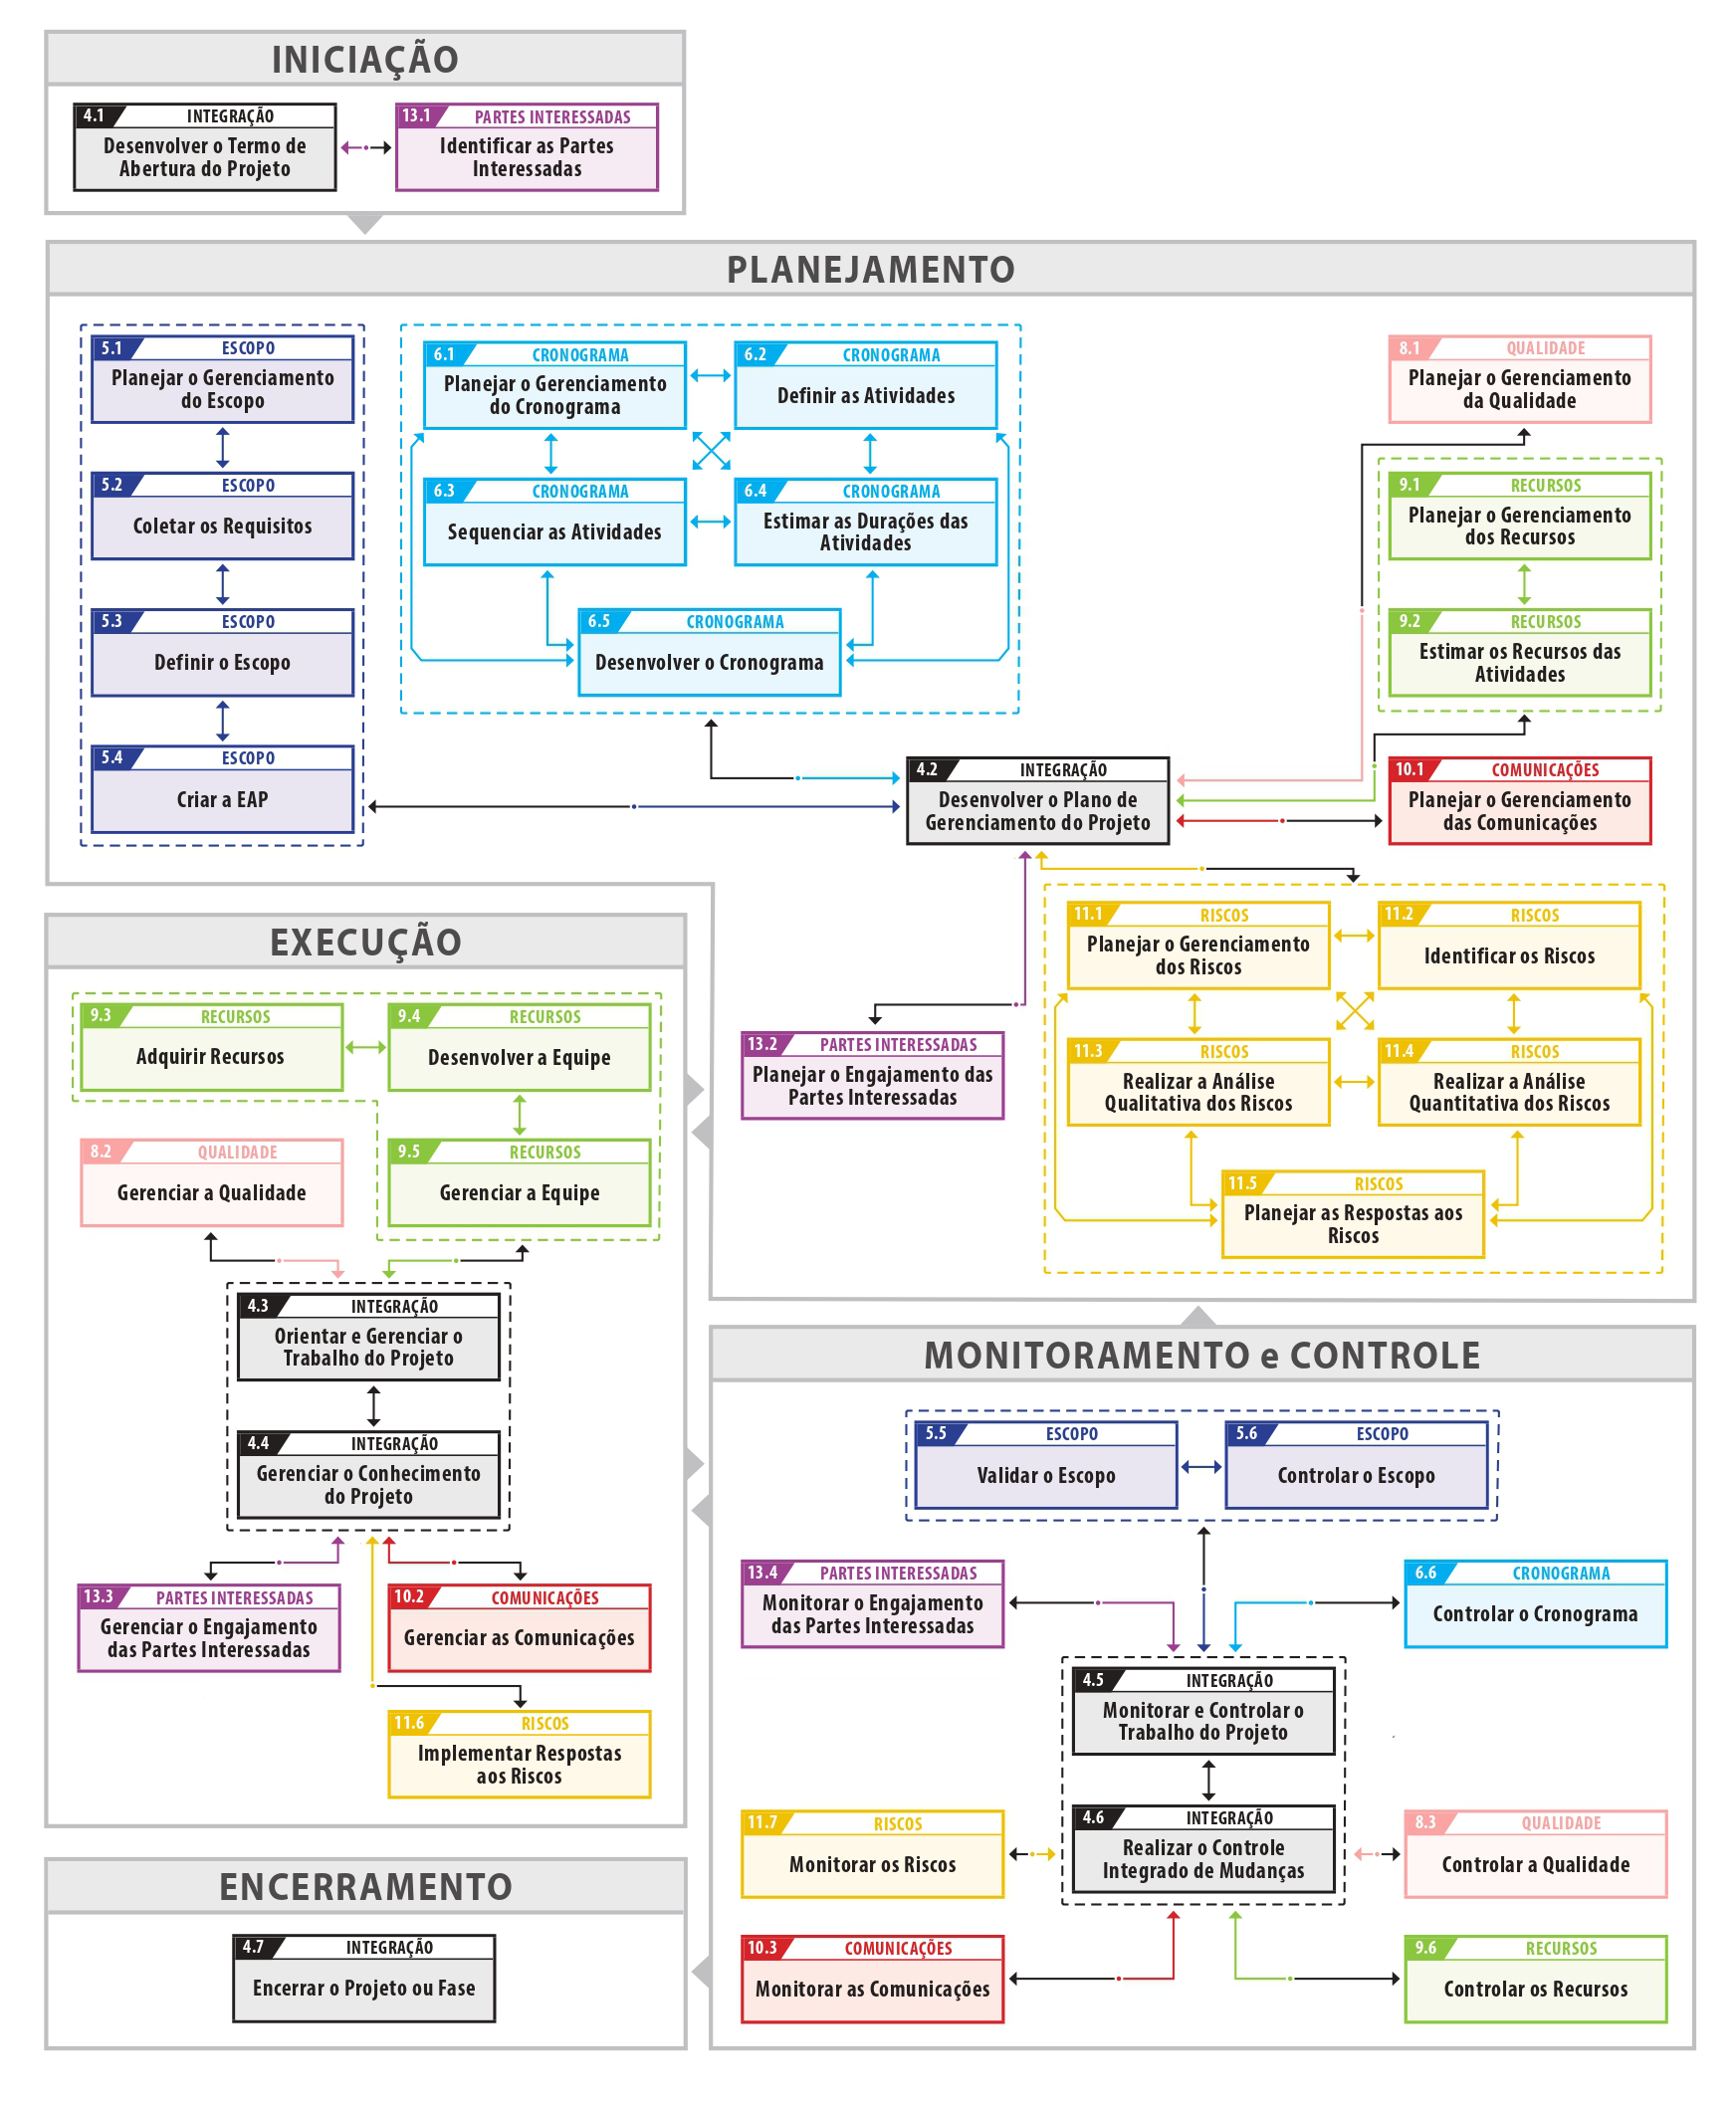
\includegraphics[scale=0.62]{Figuras/fluxo_de_processos_PMBOK}}\qquad
		
	}
	
	
\end{figure}

% ----
\subsection{EAP-  Estrutura Analita de Projetos}
% ----
O EAP e uma estrutura de forma visualizar as atividades que compõem o projeto, permitindo visualizar todo o escopo do projeto. Onde no topo fica o projeto, na segunda camada fica as etapas que no EAP e chamada de entregáveis, e para cada entregável possui as subcamadas que são as tarefas necessárias para finalizar cada uma das etapas do desenvolvimento.{\color{red} colocar referência}

 Na imagem a seguir, demostra o desenvolvimento do EAP do Projeto \textit{Smart Solution}.

\begin{figure}[H]
	\caption{\label{EAP_Smart_Solution4}EAP da \textit{Smart Solution}}
	\centering
	\mbox{%
		{
			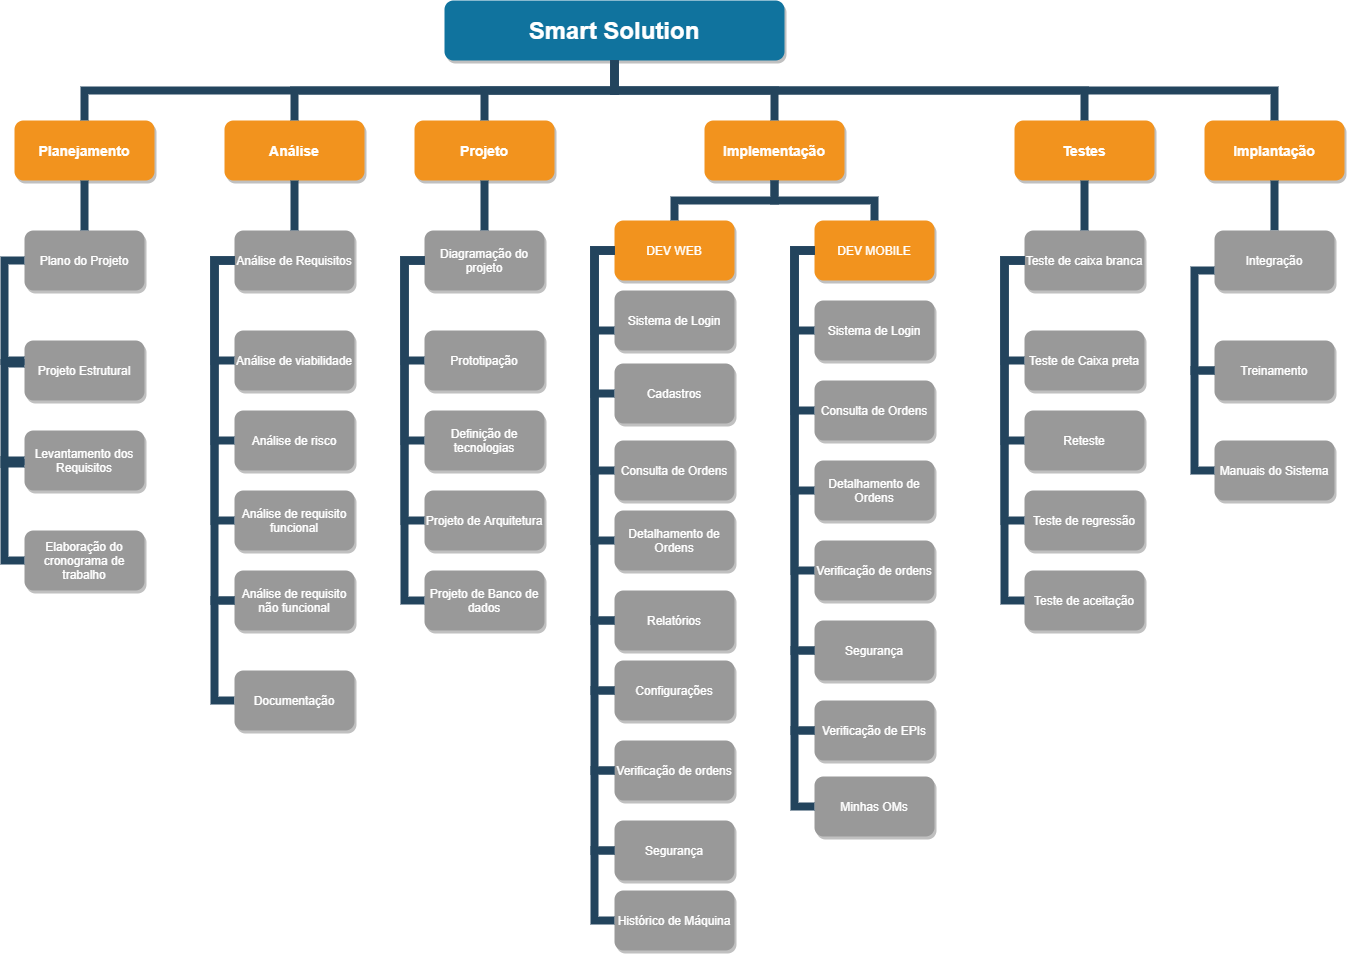
\includegraphics[scale=0.47, angle=90]{Figuras/EAP_Smart_Solution4}}\qquad
		
	}
	
	
\end{figure}
% -----

\section{Regras de Negocio}
% ---

Pode se definir regra de negócio como sendo uma norma, ou um uso comum que determina a forma de realização de uma transação que envolve uma determinada organização.\cite{alvarenga2007abordagem}
{\color{yellow} pode colocar mais uma referencia também na definição}.

{\color{red} Paragrafo bem confuso, não entendi
Sempre que uma ordem de serviço for gerada no SAP para a manutenção, esta será integrada e armazenada no sistema próprio de ordem de serviços do setor da manutenção, cada \textit{OS} gerada deverá ter um tipo de manutenção a ser realizado, esta pode ser preditiva, preventiva, rotas ou listas, toda \textit{OS} que for gerada pelo sistema SAP deverá ter um responsável atribuído no sistema, apenas este e o administrador geral do sistema terão acesso total a ordem de serviço.
Na tela \textit{“Minhas OS”}, os manutentores teram acesso as ordens que foram delegadas aos mesmos com essa ele poderá acessar mais detalhes de os, tanto para obter mais informações do serviço a ser realizado, como também ter a capacidade de realizar modificações na ordem, podendo lançar as horas trabalhadas, e organizar as operações a serem realizadas.

}

{\color{blue} Paragrafo bem confuso, muito extenso
	 
Quando um manutentor necessitar solicitar uma peça para o almoxarifado, este deve acessar a tela de solicitação de peças e realizar a solicitação, está será enviada para o almoxarifado.
Quando um manutentor decidir iniciar uma ordem de serviço, ele deverá na tela “Minhas Os” acessar a aba abertas, então escolher a ordem que deseja iniciar. Se o manutentor decidir pausar a ordem, ele deverá ir até a aba em andamento e escolher a ordem que deseja pausar.
Se o manutentor terminar o serviço a ser realizado, ele deverá ir até a tela de verificação que pode ser acessada através da tela de “detalhe de ordem de serviço”, e nessa tela ele irá realizar a verificação da ordem de serviço, para a verificação ser realizada será necessária a verificação do serviço por do solicitante e do manutentor que se responsabilizou estas podem ser realizadas na tela de verificação do sistema Mobile, o manutentor também deverá preencher informações sobre o fim da OS, como solução realizada, e informar se o serviço foi finalizado, após isso a ordem deve ser analisada pelo administrador do sistema, no sistema web, ele irá decidir se a ordem deve ser encerrada ou reaberta, para ser refeita.
O Administrador do sistema poderá através da tela de detalhe da ordem de serviço, delegar mais responsáveis em uma OS.
O Administrador do sistema terá a possibilidade de acessar a tela de relatórios, nela será possível analisar o desempenho do setor de manutenção.
O administrador poderá através do sistema web acessar uma tela de notificações.
O Administrador poderá acessar e cadastrar novos centro de custo, causa de defeito,
sintoma de defeito, tipo de máquina, componente, equipamento.

}

{\color{green} verificar os verbos e tentar melhorar o entendimento do que estão querendo passar para o leitor.
	
	
O administrador poderá acessar a tela de histórico de OS, nela será possível verificar modificações nos status da os.

Tanto o Manutentor quanto o administrador poderão acessar a tela de “Consulta de ordens”, nela será possível realizar filtros para encontrar ordens de serviço especificas.

O manutentor poderá cadastrar manualmente OS, de três tipos corretiva, preventiva, rotas e listas.

Sempre que um mecânico iniciar uma ordem de serviço será verificado os EPIs que o mesmo está utilizando, o manutentor deverá informar quais EPIs o mesmo está utilizando.
Se o manutentor pausar uma ordem, quando ele voltar, terá de preencher o Checklist de EPIs novamente informando quais EPIs ele está utilizando no momento.

O administrador poderá cadastrar novas parametrizações de segurança.
Os manutentores terão acesso aos detalhes de todas as ordens de serviço, de forma que os mesmos possam visualizar as informações pertinentes as ordens de serviço, porém sem poder realizar modificações ou alterações nas ordens de serviço que não estejam delegas para si próprio.

O administrador terá a capacidade de cadastrar tipos de operações predefinidas pela empresa, a mesmas serão utilizadas nas ordens de serviço pelos manutentores para facilitar o esboço do trabalho a ser realizado. 


}


\begin{figure}[H]
	\caption{\label{regraSimples1}Regras de Negócio Simplificada Parte 1 Da \textit{Smart Solution}}
	\centering
	\mbox{%
		{
			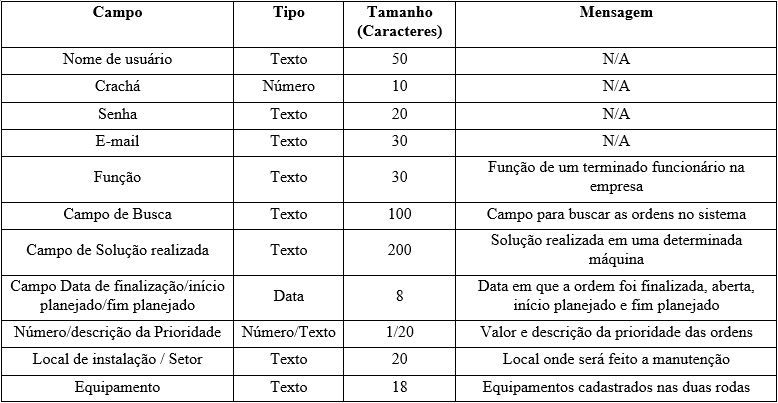
\includegraphics[scale=0.82]{Figuras/regraSimples1}}\qquad
		
	}
	
	
\end{figure}
\begin{figure}[H]
	\caption{\label{regraSimples2}Regras de Negócio Simplificada Parte 2 Da \textit{Smart Solution}}
	\centering
	\mbox{%
		{
			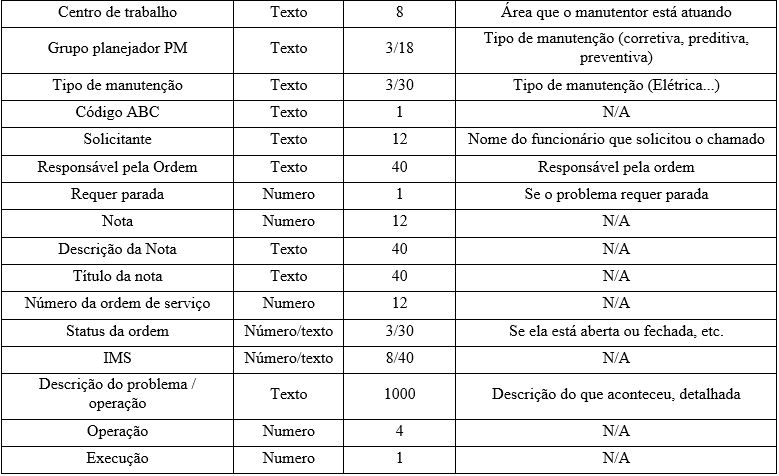
\includegraphics[scale=0.82]{Figuras/regraSimples2}}\qquad
		
	}
	
	
\end{figure}
\begin{figure}[H]
	\caption{\label{regraSimples3}Regras de Negócio Simplificada Parte 3 Da \textit{Smart Solution}}
	\centering
	\mbox{%
		{
			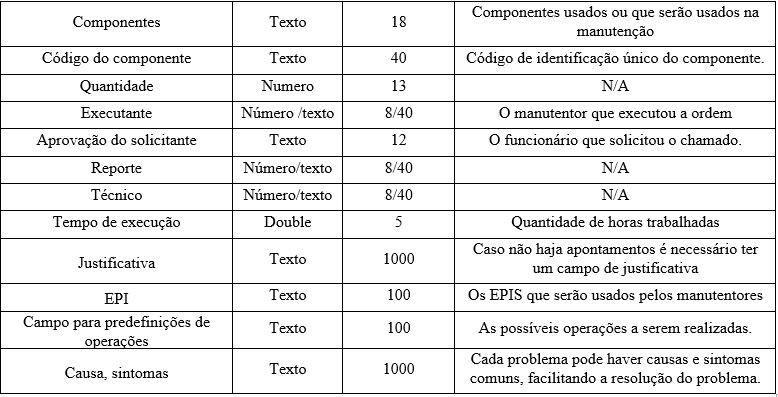
\includegraphics[scale=0.82]{Figuras/regraSimples3}}\qquad
		
	}
	
	
\end{figure}

% ---



\newpage
\section{Riscos do Projeto}
% ---
O risco em um projeto de software é uma medida da probabilidade e da perda relacionadas à ocorrência de um evento negativo que afete o próprio projeto, seu processo ou o seu produto. Em outras palavras, qualquer coisa que possa acontecer e ameaçar o bom andamento do projeto é um risco. O risco do projeto relaciona-se com
aspectos operacionais, organizacionais e contratuais. Este tipo de risco é uma responsabilidade do Gerente do Projeto, nele estando incluídos limitações de recursos, interfaces externas, relacionamentos com fornecedores e restrições
contratuais.\cite{aguiar2011gerenciando}


\begin{figure}[H]
	\caption{\label{Tabelas_riscos}Tabela de riscos do projeto \textit{Smart Solution}}
		\centering
		\mbox{%
			{
		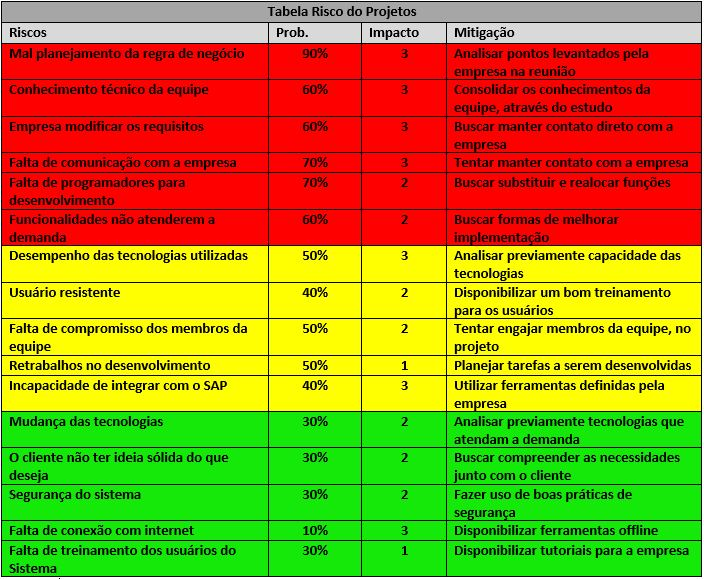
\includegraphics[scale=0.91]{Figuras/Tabelas_riscos}}\qquad
	
		}


\end{figure}

{\color{red}Descrever a tabela de riscos, os pontos mais críticos}

% ----
\section{Diagrama de Causa e Efeito}
% -----

{\color{red} Utilizar referencia
	
O diagrama de causa e efeito ou espinha de peixe, e utilizado para estruturar causas para um determinado efeito e encontra as áreas onde podem ser introduzido melhorias, mais também pode ser utilizado controlar o processo e garantir qualidade no produto final, assim como relacionar um defeito com as suas causas.} Neste projeto foi utilizado esse diagrama para localizar os possíveis problemas que podem afetar o processo de desenvolvimento e conclusão do desenvolvimento do software. Na figura abaixo mostra o diagrama de causa e efeito da \textit{Smart Solution}.

\begin{figure}[H]
	\caption{\label{smart_solution_espinha_de_peixe}Diagrama de Causa e Efeito da \textit{Smart Solution}}
	\centering
	\mbox{%
		{
			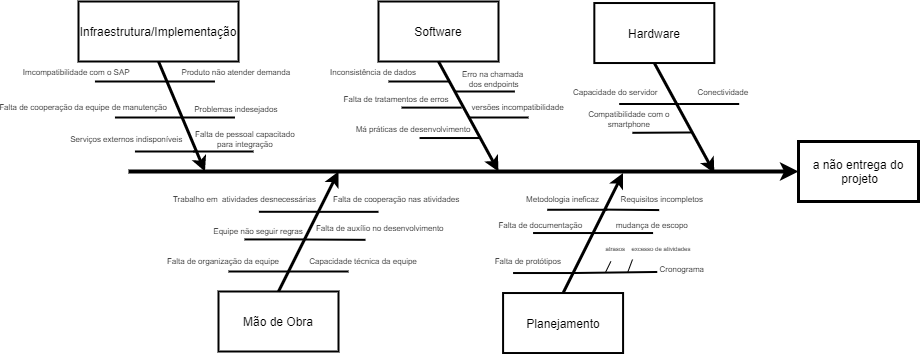
\includegraphics[scale=0.70, angle=90]{Figuras/smart_solution_espinha_de_peixe}}\qquad
		
	}
	
	
\end{figure}

{\color{red} Descrever brevemente o diagrama}

% ---
\chapter{Requisitos do Sistema}
% ---

Para que o sistema possa atender as demandas da Duas Rodas serão necessários alguns requisitos não só para um bom funcionamento do sistema, como também para tornar o projeto utilizável pela empresa, uma vez que os requisitos essenciais não sejam atendidos o projeto pode se tornar inviável para a implementação no setor da mecânica.
% ---


\section{Requisitos Funcionais}
% --- 
%O Smart Solution realizará o gerenciamento das ordens de serviço, distribuição delas via mobile para os mecânico, gerir a quantidade de peças no estoque, permitir que o mesmo solicite novas peças se necessário, consultar ordens de serviços de acordo com seu status (abertas, em andamento e finalizadas), armazenar assinaturas digitais através do número do crachá do funcionário, também possuirá funcionalidades extras como registro manual de funcionários e chamados de manutenção.
Os requisitos funcionais tratam de aspectos comportamentais do software.\cite{alvarenga2007abordagem}


\begin{figure}[H]
	\caption{\label{parte1funcional}Requisitos Funcionais Parte 1 Da \textit{Smart Solution}}
	\centering
	\mbox{%
		{
			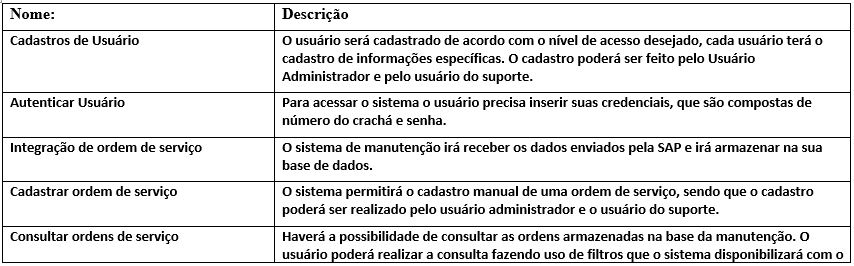
\includegraphics[scale=0.76]{Figuras/parte1funcional}}\qquad
		
	}
	
	
\end{figure}
\begin{figure}[H]
	\caption{\label{parte2funcional}Requisitos Funcionais Parte 2 Da \textit{Smart Solution}}
	\centering
	\mbox{%
		{
			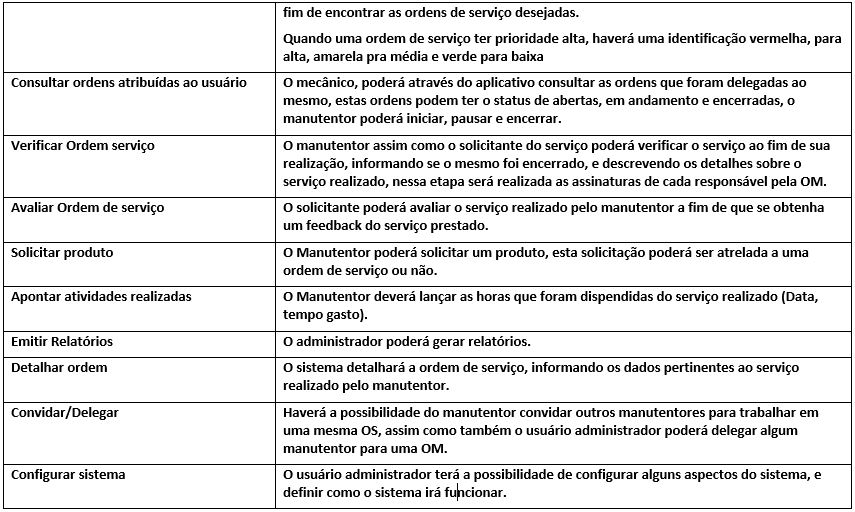
\includegraphics[scale=0.76]{Figuras/parte2funcional}}\qquad
		
	}
	
	
\end{figure}
\begin{figure}[H]
	\caption{\label{parte3funcional}Requisitos Funcionais Parte 3 Da \textit{Smart Solution}}
	\centering
	\mbox{%
		{
			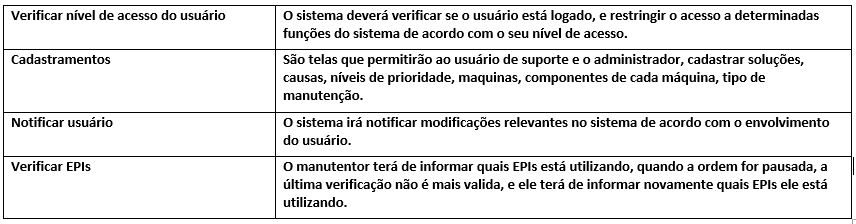
\includegraphics[scale=0.76]{Figuras/parte3funcional}}\qquad
		
	}
	
	
\end{figure}


%definiçao
%O \textit{Smart Solution} realizará o gerenciamento das ordens de serviço, distribuição delas via mobile para o mecânico, gerir a quantidade de peças no estoque, permitir que o mesmo solicite novas peças se necessário, consultar ordens de serviços de acordo com seu status (abertos, em andamento e finalizadas), armazenar assinaturas digitais através do número do crachá do funcionário, também possuirá funcionalidades extras como registro manual de funcionários e chamados de manutenção.



% ---
%\section{Requisitos Não-Funcionais}
% ---
\newpage
\section{Requisitos não Funcionais}
% ---
Os requisitos não-funcionais são as condições de comportamento e as restrições que 
Já os requisitos não-funcionais dizem respeito às condições de comportamento e restrições que devem prevalecer no software como, por exemplo, "o tempo de geração e emissão do relatório mensal que demonstra o histórico das transações comerciais de uma propriedade rural não deve ultrapassar 5 minutos". Neste exemplo, citamos um requisito de performance (ou um atributo de qualidade) que o software deve atender.\cite{alvarenga2007abordagem}


\begin{figure}[H]
	\centering
	\mbox{%
		{\label{reqnaofuncional}%
			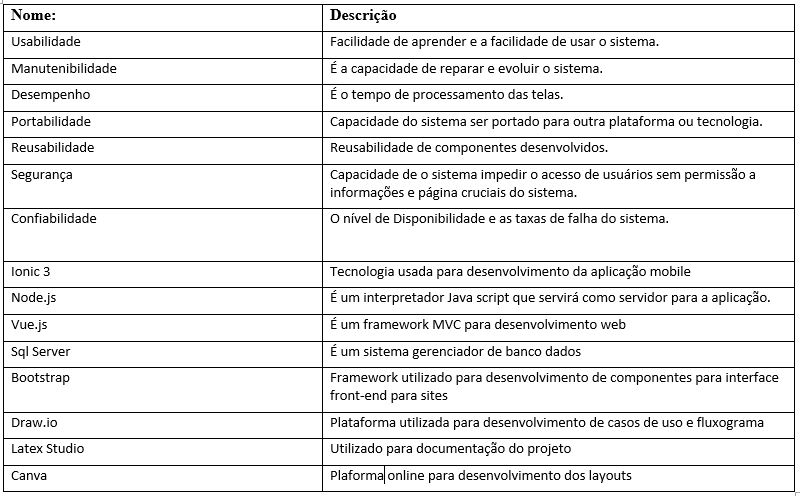
\includegraphics[scale=.80]{Figuras/reqnaofuncional}}\qquad
		

		}
	
	
\end{figure}
%(textyo a ser anexado)

% ---
\newpage
	


\section{Métricas}
% ---

Na concepção das ideias para desenvolver o \textit{Smart Solution}, foi utilizado primeiramente uma base fornecida pela empresa como as folhas de ordens de serviços, informações adicionais fornecidas no dia, após isso surgiu novas ideias como design, forma de colher as assinaturas, segurança, autenticação de usuário, ferramentas que melhor se encaixam com a proposta de software que seria desenvolvido. Agora as novas ideias são remover algumas telas e funcionalidades de teste que foram adicionadas na aplicação móvel, tais como: telas de cadastro de usuário e cadastro de ordem de serviço, e aplicá-las na versão web, pois caso algum recurso do SAP não estiver funcionando isso pode influenciar negativamente na abertura de chamados e integração com o \textit{Smart Solution}, dessa forma o sistema desenvolvido suprirá a parada inesperada do SAP ou qualquer outra fonte que afete a abertura de chamados. 
% ---
\newpage
\section{Cronograma}
% ---
Análise de requisitos, Planejamento, atribuição de tarefas,
desenvolvimento do layout do sistema, desenvolvimento da aplicação server,teste de implementação, finalização do projeto, testes para a implementação. Foram etapas para o desenvolvimento da documentação e implementação do projeto.


\begin{figure}[H]
	\caption{\label{Cronograma_marco_e_Abril}Cronograma para o desenvolvimento em março e Abril do projeto \textit{Smart Solution}}
	\begin{center}
		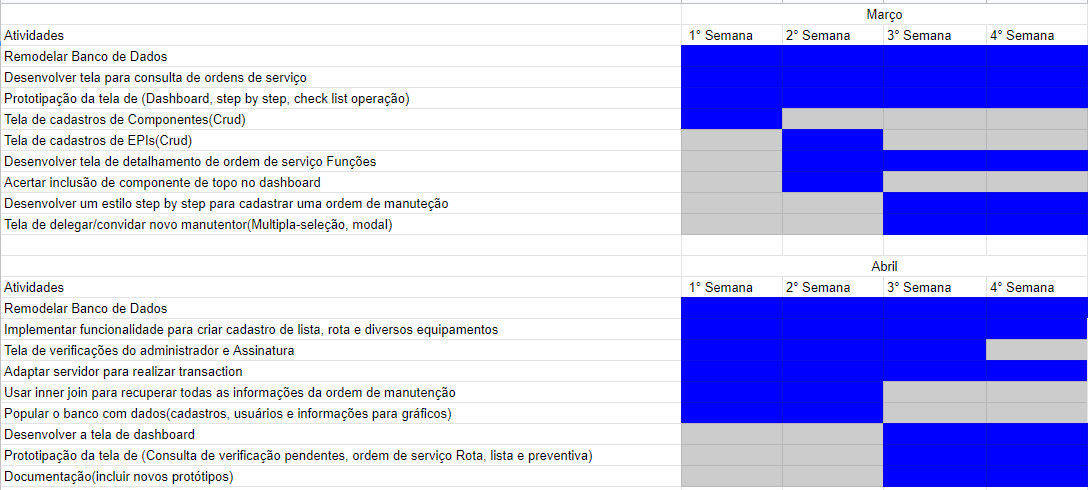
\includegraphics[scale=0.85,angle=90]{./Figuras/Cronograma_marco_e_Abril}
	\end{center}
	
\end{figure}
%----

\begin{figure}[H]
	\caption{\label{Cronograma_maio_e_Junho}Cronograma para o desenvolvimento em maio e junho do projeto \textit{Smart Solution}}
	\begin{center}
		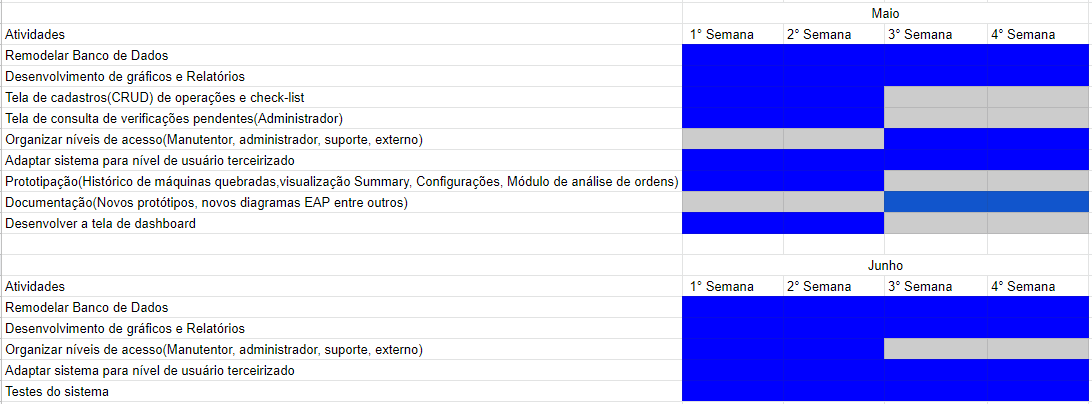
\includegraphics[scale=0.85,angle=90]{./Figuras/Cronograma_maio_e_Junho}
	\end{center}
	
\end{figure}
% ---

\chapter{Anterioridade}
%Com o desenvolvimento do presente trabalho, ficou visível que muitas das funcionalidades presentes no sistema, já existem, há vários sistemas de ordens de serviço e gestão de manutenção no mercado atualmente, a seguir será elencado alguns dos destaques no mercado atualmente.
Com o desenvolvimento do presente trabalho, ficou visível que muitas das funcionalidades presentes no sistema, já existem. Há vários sistemas de ordens de serviço e gestão de manutenção atualmente no mercado, a seguir será elencado alguns dos destaques no mercado atualmente.

O sistema da \textit{Auvo} é um sistema de gestão de manutenção, com a capacidade de geração de ordens de manutenção, controle das ordens, relatórios de execução, porém diferente do
projeto apresentado neste documento. O sistema do Auvo é um pouco mais abrangente,
Gestão de orçamentos e cálculo de reembolso de despesas.\cite{Auvo2019}

Outro sistema que também destaca-se, é o \textit{Umov} 
, que permite a geração de ordens de serviço,
os diferenciais deste sistema são o sistema de Geolocalização, Checklists de atividades \cite{umov2019}.

O sistema \textit{Smart Solution}, diferente dos apresentados anteriormente por ser mais específico para as
necessidades da empresa Duas Rodas, assim com design personalizado, desempenho melhor em seus processos.

% dessa forma acaba não trazendo algumas
%funcionalidades, principalmente em questões financeiras, porém algumas dessas
%podem vir a ser implementadas no presente projeto.

%\cite{batsim2018}
%\section{teste}
\chapter{Análise e Design}

%Neste capitulo temos como objetivo analisar e detalhar a solução  de acordo com os requisitos pedidos pela empresa  levantados no capitulo 3.Por isso devemos ter uma visão geral da arquitetura e modelagem que devera ser utilizada, através dos diagramas.
Neste capítulo tem como objetivo analisar e detalhar a solução de acordo com os requisitos pedidos pela empresa que foram  levantados anteriormente. Para isso foi necessária uma visão geral da arquitetura e modelagem que foi representada  utilizada, através dos diagramas
\newpage
\section{Fluxograma}

A melhor definição de fluxograma é “um mapa gráfico rico em informações que descreve claramente as etapas do processo, suas tomadas de decisão, fornecendo documentação onde for necessário”.\cite{Gradus2019}.

{\color{red} Adicionar mais uma referencia de fluxograma, ou referenciar o que citaram abaixo} 

Além da descrição citada, é importante observar que há muitas razões para se usar o fluxograma, por exemplo:
\begin{itemize}
	\item Melhorar o entendimento do processo através do apelo visual;
	\item Diagnosticar onde se necessita melhorias;
	\item Mostrar a sequência em que as etapas são executadas, permitindo identificar ações que possam ser eliminadas;
	\item Identificar melhorias que podem ser feitas imediatamente;
	\item Descreve qualquer tipo de processo, dos simples aos complexos;
	%\item
	\item Detalha o funcionamento de todas as partes do processo;
	\item Fácil uso
	\item Fácil interpretação
\end{itemize}
\newpage


\begin{figure}[H]
	\caption{\label{fluxograma2teste}Fluxograma da\textit{ Smart Solution}}%
	\begin{center}
		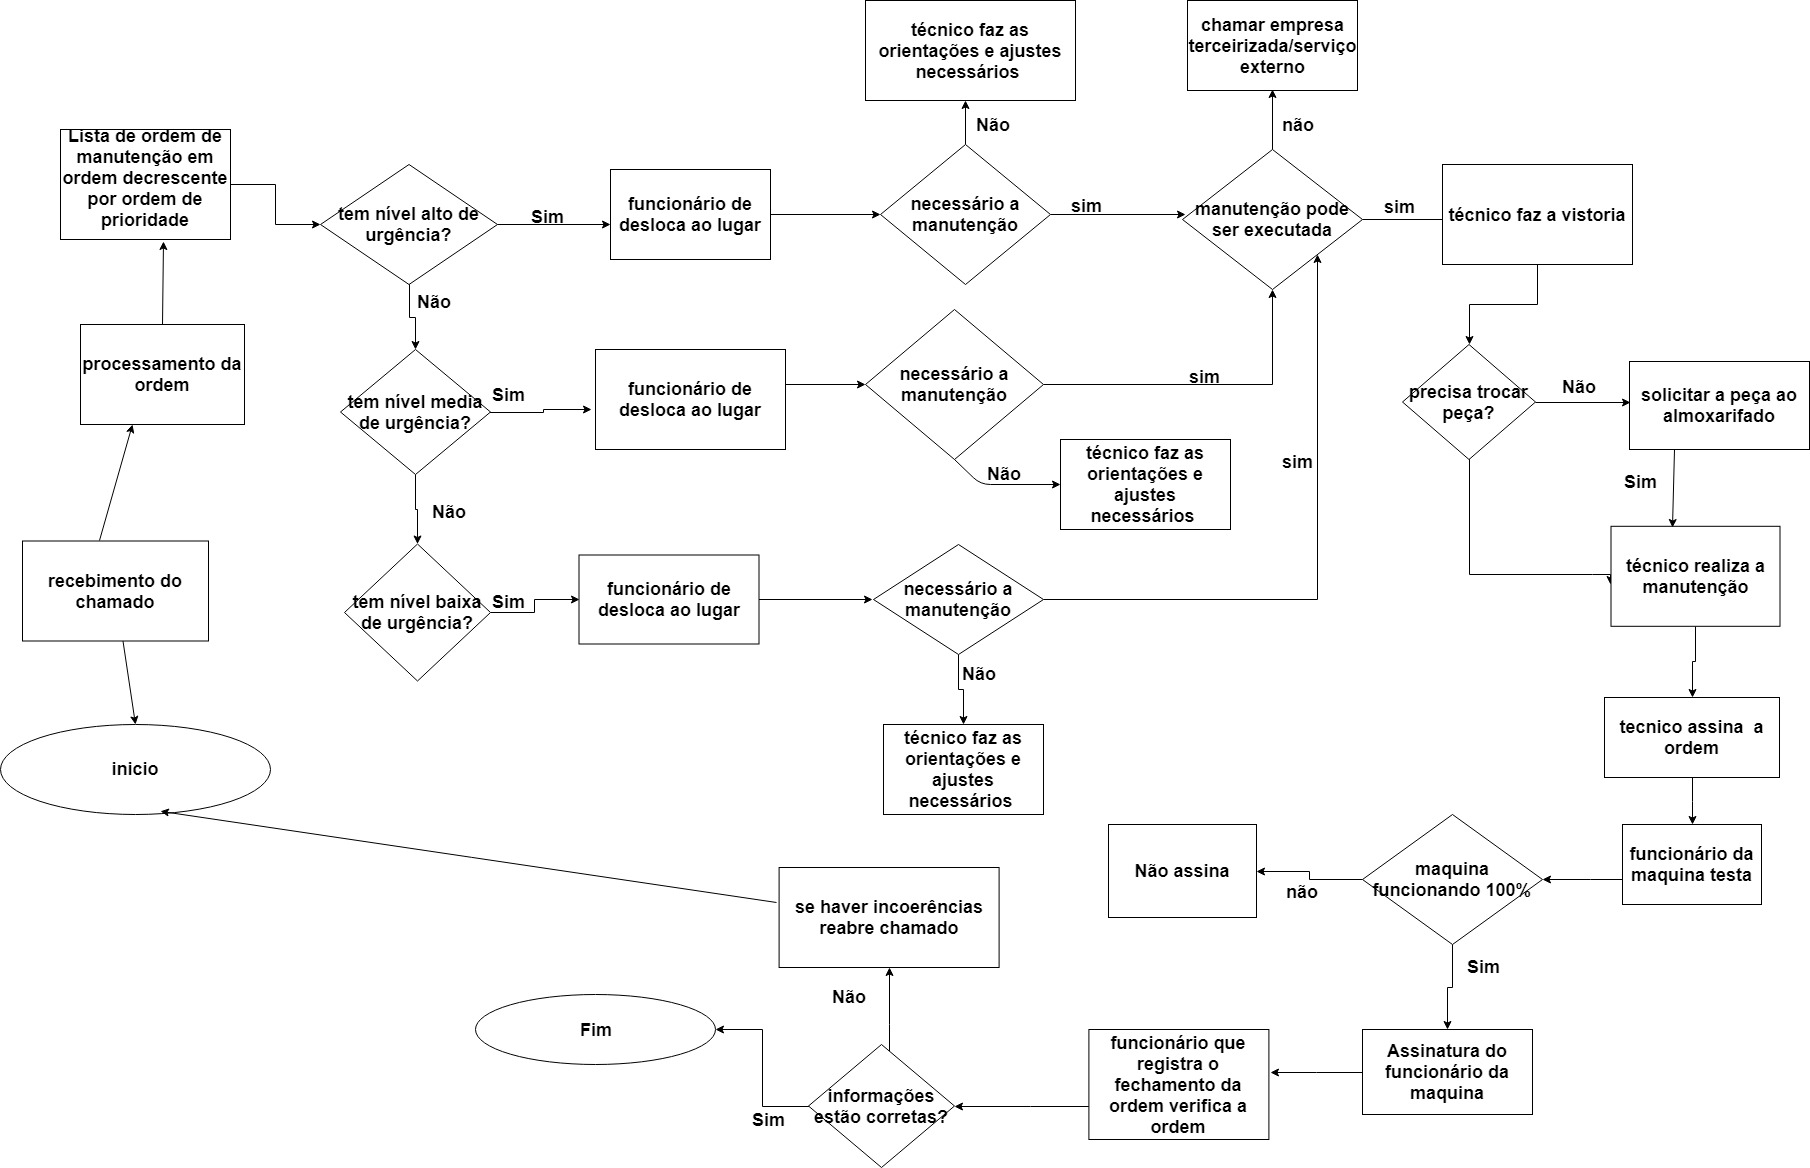
\includegraphics[scale=0.40,angle=90]{Figuras/fluxograma2teste}
		
	\end{center}
	%	\legend{Fluxograma do Sistema}
\end{figure}
\newpage


Na Figura \ref{fluxograma2teste} percebe-se que o fluxo começa recebendo a ordem de serviço do SAP e vai para o processamento para colocar em sua lista de prioridades designada, após isso é verificado se precisa que o técnico se desloque até a máquina ou apenas orientar o usuário os procedimentos a adotar, mas se for necessário técnico faz a vistoria e verifica de precisara de peça ou não , após isso o funcionário da máquina faz a vistoria  em seguida e coletado as assinaturas e se estiver tudo certo fecha a ordem de serviço.

\newpage

\section{Diagrama de Caso de Uso}
% ---

O diagrama de casos de uso é o diagrama mais geral e informal, utilizado normalmente nas fases de levantamento e análise de requisitos do sistema, embora venha a ser consultado durante todo o processo de modelagem e possa servir de base para outros diagramas. Apresenta uma linguagem simples e de fácil compreensão para que os usuários possam ter uma ideia geral de como o sistema irá se comportar. Procura identificar os atores (usuários, outros sistemas ou até mesmo algum hardware especial) que utilizarão de alguma forma  o software, bem como os serviços, ou seja, as funcionalidades que o sistema disponibilizará aos atores, conhecidas nesse diagrama como casos de uso.\cite{guedes2009uml}

 {\color{red}Adicionar mais uma referencia}
 
\begin{figure}[H]
	\caption{\label{novocasodeusointegra}Diagrama de Caso de Uso Desenvolvido para o projeto Smart Solution}
	\begin{center}
		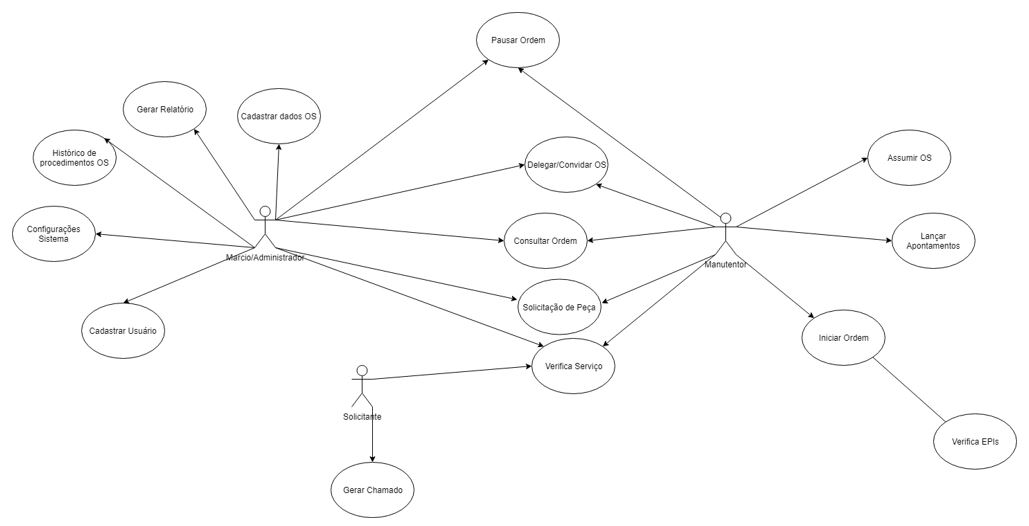
\includegraphics[scale=0.90,angle=90]{./Figuras/novocasodeusointegra}
		
	\end{center}
	%	\legend{Diagrama de Caso de Uso}
\end{figure}

\newpage
%descriçao caso de uso
{\color{red}Adicionar label na descrição, com fiz na figura 5.1; melhorar a descrição do caso de uso, retirar o nome do usuário.


}

O caso de uso possui como atores administrador geral de TI, márcio, responsável pela máquina e manutentor. O administrador tem visão geral de todas as informações provenientes das ordens de serviços como de seus procedimentos, históricos disponíveis. O márcio faz a atribuição das ordens de serviço assim como a impressão e pós realização confere a ordem de serviço para assim assinar e retornar ao SAP as informações contidas na ordem de serviço. O responsável da máquina e responsável por uma das assinaturas mediante uma vistoria de sua máquina de uso. O manutentor realiza a manutenção e solicita peças ao almoxarifado se for necessário a troca de alguma peça.



\section{Diagrama de Classes}
%---
O diagrama de classes é o mais utilizado e é um dos mais importantes aplicados na UML. Serve de apoio para a maioria dos demais diagramas. Como o próprio nome diz, define a estrutura das classes utilizadas pelo sistema, determinando os atributos e métodos que cada classe tem, além de estabelecer como as classes se relacionam e trocam informações entre si.\cite{guedes2009uml}

{\color{red} Adicionar mais uma referência}

\newpage
\begin{figure}[H]
	\caption{\label{Diagrama_de_classe_integrado}Diagrama de classe para \textit{Smart Solution}}
	\begin{center}
		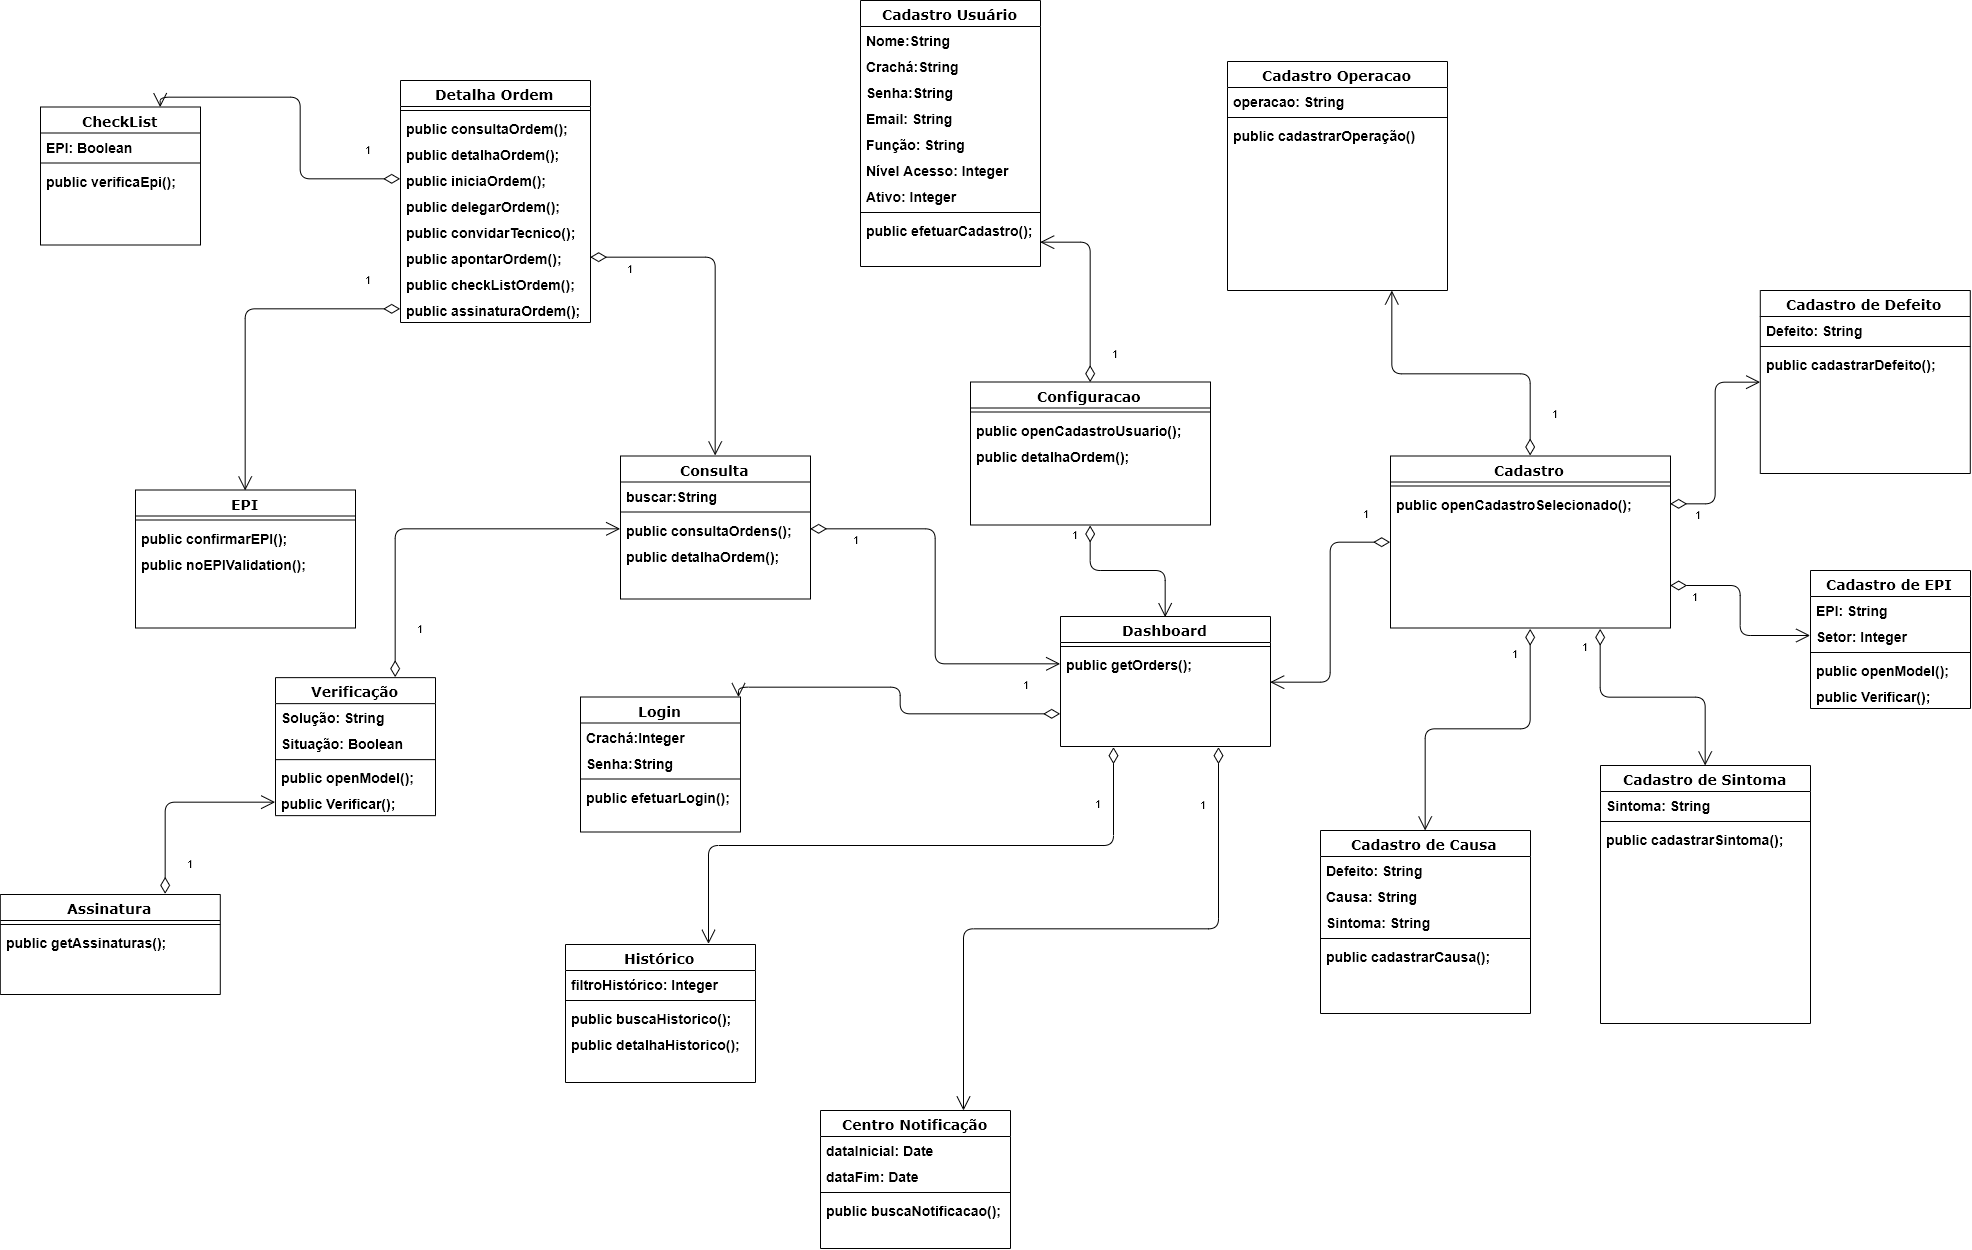
\includegraphics[scale=0.35, angle=90]{./Figuras/Diagrama_de_classe_integrado}
		
	\end{center}
	%	\legend{Diagrama de Classe}
\end{figure}

\newpage


{\color{red}Adicionar label na descrição, com fiz na figura 5.1;}

Neste diagrama está a base das classes do projeto\textit{ Smart Solution} , visando ter telas com suas regras de negócio variáveis que o sistema deveria ter, além de começarmos a modelar possíveis dados recebidos. Dentro desta base temos uma classe de login para usuário efetuar o mesmo, banco de dados para armazenamento das ordens de manutenção , assinaturas para finalidade de pegar as assinaturas de cada responsável pelo processo , outras telas como setor solicitante, equipamento que está com problemas e solicitar peças do estoque ,dados da manutenção que e recebido via SAP.

\newpage
\section{Diagrama de Atividades}


O diagrama de atividade preocupa-se em descrever os passos a serem percorridos para a conclusão de uma atividade específica, podendo esta ser representada por um método com certo grau de complexidade, um algoritmo, ou mesmo por um processo completo. O diagrama de atividade concentra-se na representação do fluxo de controle de uma atividade.\cite{guedes2009uml}. COmo é representado na Figura \ref{diagramaDeAtividades}.

{\color{red} Atulizar o diagrama de atividades de vcs}

\begin{figure}[H]
	\caption{\label{diagramaDeAtividades}Diagrama de Atividades no desenvolvimento do software \textit{Smart Solution}}
	\begin{center}
		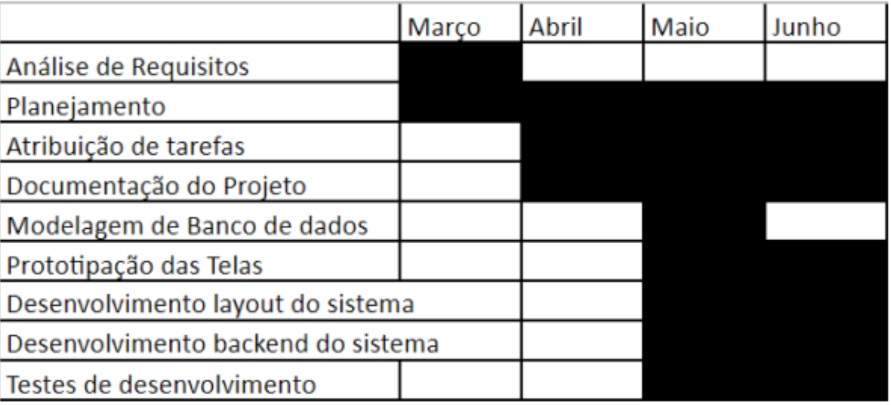
\includegraphics[scale=0.72 ]{./Figuras/diagramaDeAtividades}
		
	\end{center}
	%	\legend{Diagrama de Atividades}
\end{figure}
%\section{Diagrama de Sequencia}
%\section{Modelo de Dados}
%\subsection{Modelo Lógico da Base de Dados}
%\subsection{Criação física do Modelo de Dados}
%\subsection{Dicionário de Dados}
\newpage
\section{Ambiente de Desenvolvimento}


%36Capítulo 4.  Análise e DesignÉ uma plataforma utilizada para o desenvolvimento de aplicações Web.-Node Js: Interpretador de código javascript. -Ionic: Utilizado para o de-senvolvimento de aplicativos móveis híbridos. Git: Sistema de controle deversões distríbuido, é utilizado para o versionamento de código.
%Foi utilizado minha maquina que possui SSD 240 gb processador i3 com 4 gigas de RAM , mause teclado configuração semelhante dos meus companheiros.
%Também foi utilizado para desenvolver o software , a sala de aula, em casa, grupo de whatsapp e gitHub para todos terem a ultima versão.

{\color{red} Adicionar uma breve introdução antes das ferramentas utilizadas}

As linguagens utilizadas foram  as seguintes: Javascript - Uma linguagem de alto nível, dinâmica e fracamente tipada, muito utilizada atualmente; TypeScript - Um superconjunto de Javascript que traz várias adições a linguagem, foi desenvolvido pela Microsoft; Tecnologias Utilizadas - MySQL: Utilizada para o gerenciamento de dados; Angular: É uma plataforma utilizada para o desenvolvimento de aplicações Web; Node.Js: Interpretador de código javascript; Ionic: Utilizado para o desenvolvimento de aplicativos móveis híbridos; Git: Sistema de controle de versões distribuído, é utilizado para o versionamento de código. Para que houvesse o desenvolvimento mútuo do projeto se fez necessário um ambiente adequado com as ferramentas necessárias, das quais o SENAI foi responsável por fornece-las.


\section{Sistemas e Componentes Externos Utilizados}

%GitHub: Plataforma de hospedagem de código fonte, nela serão armazenados os códigos do projeto, facilitando o acesso a diferentes versões de desenvolvimento aos desenvolvedores.

{\color{red} Melhorar esta descrição}


GitHub do Smart Solution \footnote{\url{https://github.com/senai-duasrodas}}: Plataforma de hospedagem de código fonte, nela serão armazenados os códigos do projeto, facilitando o acesso a diferentes versões de desenvolvimento aos desenvolvedores, possibilitando o desenvolvimento em conjunto de toda a equipe.

\newpage


\chapter{Protótipo}
%---
No desenvolvimento de um produto, podem ser entendidas
duas formas de design: a conceitual e a física. Enquanto a
conceitual preocupa-se em estabelecer bases que permitam o
entendimento do comportamento e finalidade do produto, a
física procura estabelecer detalhes de design, como tamanho,
elementos e outros fatores.\cite{medeiros2013importancia}

%Figura "a", tela com finalidade de logar o usuário.
%Figura "b", tela para cadastrar usuário .
%\ref{login}
\newpage
\begin{center}
	Protótipos da parte Mobile.
\end{center}

%Tela com finalidade de logar o usuário.
Tela de login onde o funcionário em seu dispositivo mobile, onde ele efetuará a entrada em nosso sistema utilizando-se o numero de crachá e senha previamente cadastrado no sistema.


\begin{figure}[htb]
	\centering
	\mbox{%
		\subfigure[Tela Login]{\label{Login}%
			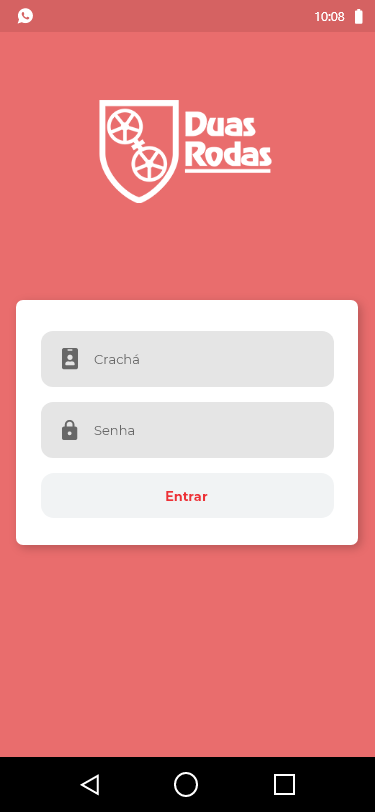
\includegraphics[scale=.65]{Figuras/Login}}\qquad
		
	}	
\end{figure}
\newpage
%--
%Tela de Menu parte superior da tela com informações rápidas sobre ordens de serviços.
Tela de menu foi dividida em duas imagens. Está primeira refere-se a parte superior do menu que contem gráficos para o funcionário acompanhar as ordens em aberto,andamento, e um gráfico maior que pode acompanhar uma visão geral do mês das ordens de serviços.  
\begin{figure}[htb]
	\centering
	\mbox{%
		\subfigure[Tela Menu parte superior da tela]{\label{MENU}%
			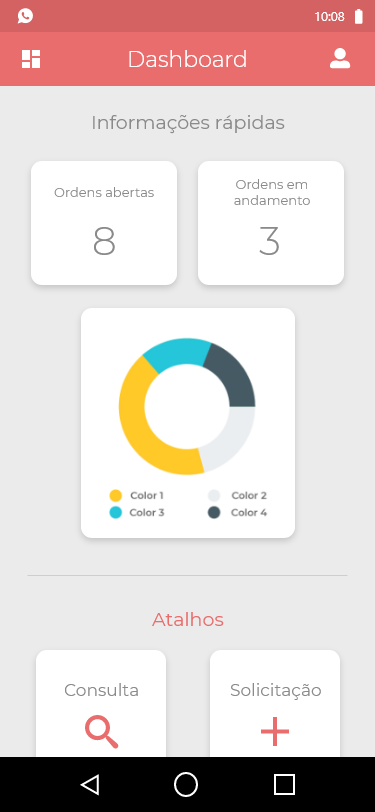
\includegraphics[scale=.65]{Figuras/MENU}}
	}	
	
\end{figure}
% ---
\newpage
%Figura "a", tela principal com finalidade de mostrar todas as opções do usuário.
%Figura "b", tela para cadastramento de ordem de serviços.
%Tela de Menu parte inferior da tela com finalidade de acesso rápido de cada operação disponível.
Tela de menu segunda imagem, que corresponde aos atalhos para um rápido acesso aos recursos disponíveis do sistema para o funcionário
como consultar ordens de serviço, cadastrar causa,sintoma ou defeito,
solicitar peça para o estoque entre outros recursos.
%\ref{dashboard}
\begin{figure}[htb]
	\centering
	\mbox{%
		\subfigure[Tela Menu parte inferior da tela]{\label{MENU_1}%
			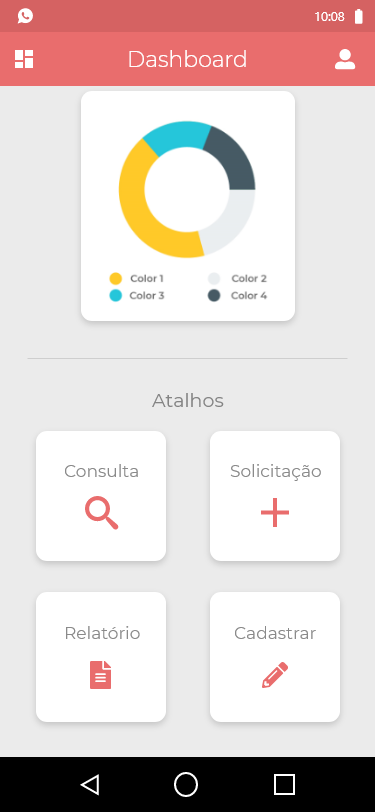
\includegraphics[scale=.65]{Figuras/MENU_1}}
	}	
	
\end{figure}
%--
\newpage
Tela de para cadastrar causa dos problemas da OS e de seus sintomas.
\begin{figure}[htb]
	\centering
	\mbox{%
		\subfigure[Tela defeito e sintoma]{\label{CADASTROS_1}%
			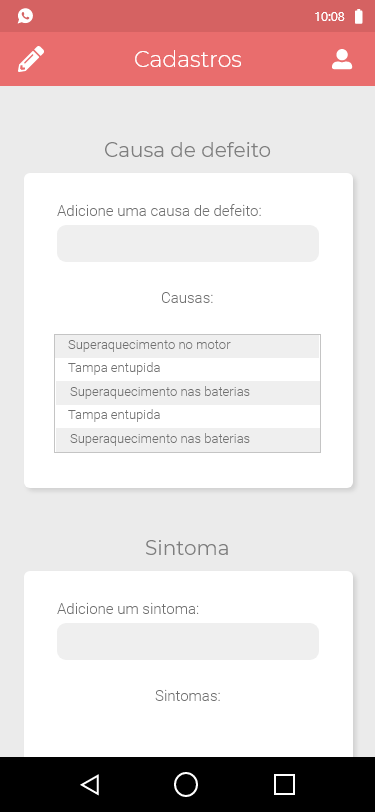
\includegraphics[scale=.65]{Figuras/CADASTROS_1}}\qquad
		
	}
\end{figure}
% ---
\newpage
%Figura "a", telas com finalidades de consultar Ordem Serviço.
%Figura "b", tela para ver os detalhes de cada Ordem de Serviço.
Tela de com opções de detalhamento de ordem de serviço.
%\ref{consulta}
\begin{figure}[htb]
	\centering
	\mbox{%
		
		\subfigure[Tela de opções de Detalhes]{\label{DETALHES_OS_1}%
			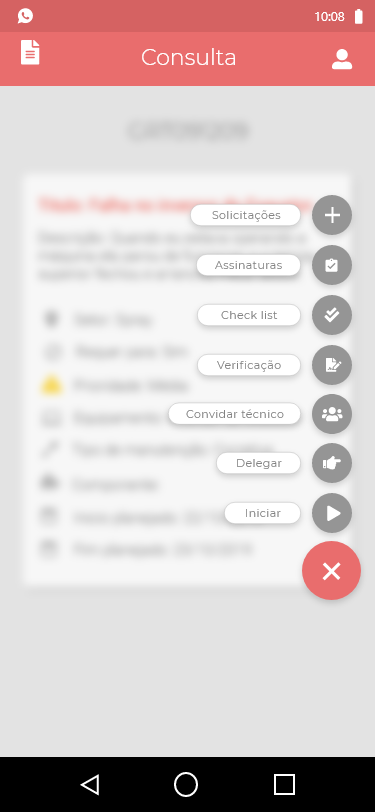
\includegraphics[scale=.65]{Figuras/DETALHES_OS_1}}
	}
	
\end{figure}
\newpage
Tela de cadastro de defeitos apresentados na manutenção também como suas causas de defeito. 
\begin{figure}[htb]
	\centering
	\mbox{%
		\subfigure[Tela de defeito e causa]{\label{CADASTROS}%
			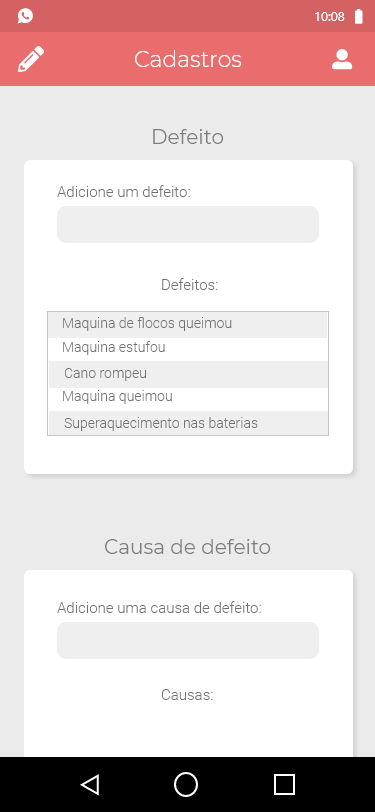
\includegraphics[scale=.65]{Figuras/CADASTROS}}\qquad
		
	}	
\end{figure}
% ---
%\newpage
\newpage
Tela de detalhamento mostrando todos os detalhes da OS.
%Figura "a", telas para verificação de ordem de serviço.
%Figura "b", tela para pegar assinatura dos responsáveis por meio do número do crachás.

%\ref{verificacao}
\begin{figure}[htb]
	\centering
	\mbox{%
		\subfigure[Tela de consulta detalhada]{\label{DETALHES_OS}%
			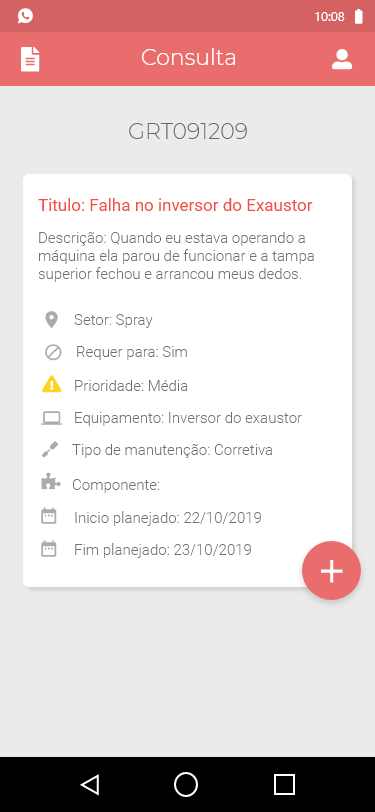
\includegraphics[scale=.65]{Figuras/DETALHES_OS}}\qquad
		
	}	
\end{figure}
\newpage
%--
Tela de consultar de ordens de serviço com filtros por data ,prioridade, status ou suas próprias em minhas os.
\begin{figure}[htb]
	\centering
	\mbox{%
		\subfigure[Tela consultar OS]{\label{CONSULTAR_OS}%
			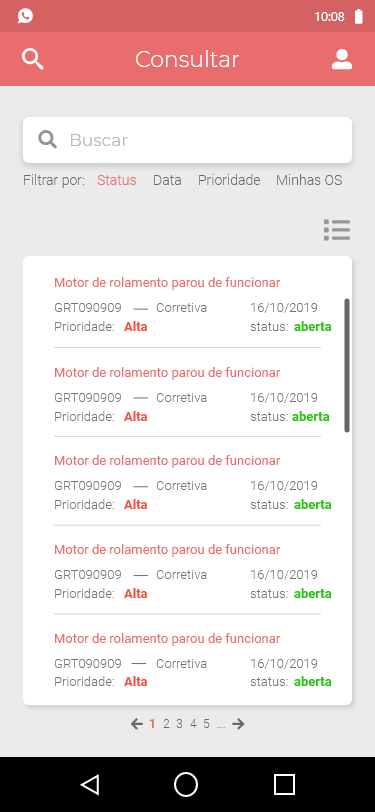
\includegraphics[scale=.65]{Figuras/CONSULTAR_OS}}
	}
\end{figure}
% ---

%Figura "a", telas com finalidade de solicitação de peças.
%Figura "b", tela para realizar apontamento pelo mecânico.
\newpage
Tela para ser solicitada peças para manutenção.

\begin{figure}[htb]
	\centering
	\mbox{%
		\subfigure[Tela Solicitação de Peça]{\label{SOLICITACOES_DE_PECAS}%
			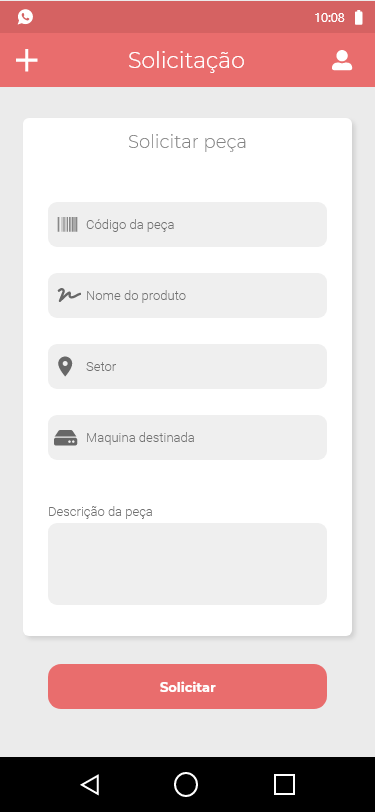
\includegraphics[scale=.65]{Figuras/SOLICITACOES_DE_PECAS}}\qquad
	}
	
\end{figure}
\newpage
Tela de verificação, apontamento e assinatura para realizar o funcionário se o problema foi resolvido, apontar horas trabalhadas e coletar assinatura.
\begin{figure}[htb]
	\centering
	\mbox{%
		
		\subfigure[Tela Verificação]{\label{VERIFICACAO}%
			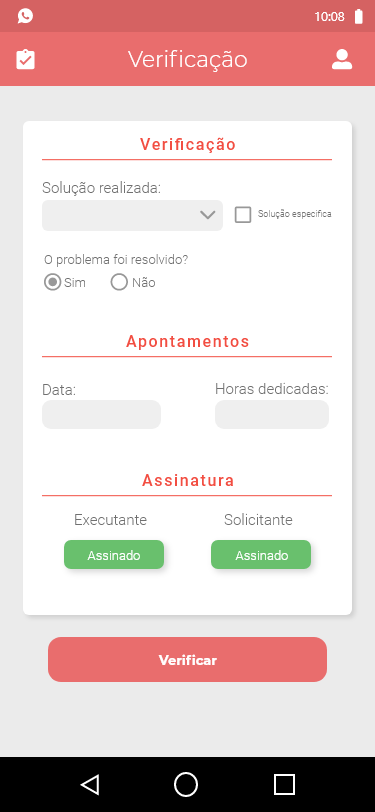
\includegraphics[scale=.65]{Figuras/VERIFICACAO}}
	}	
	
\end{figure}
\newpage

Tela de verificação mostrando o processo de assinatura do executante e do seu solicitante.

\begin{figure}[htb]
	\centering
	\mbox{%
		\subfigure[Tela Verificação Assinatura]{\label{VERIFICACAO_2}%
			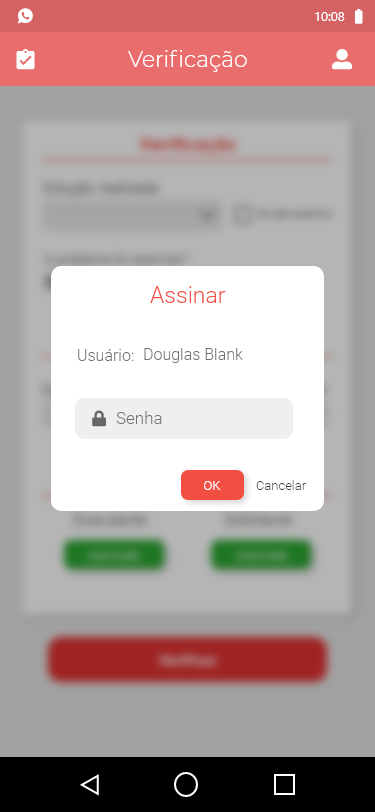
\includegraphics[scale=.65]{Figuras/VERIFICACAO_2.png}}\qquad
	}	
	
\end{figure}
\newpage
Tela das assinaturas para verificar se o processo teve a aprovação dos responsáveis em cada etapa realizada.

\begin{figure}[htb]
	\centering
	\mbox{%
		\subfigure[Tela Apontado]{\label{ASSINATURAS}%
			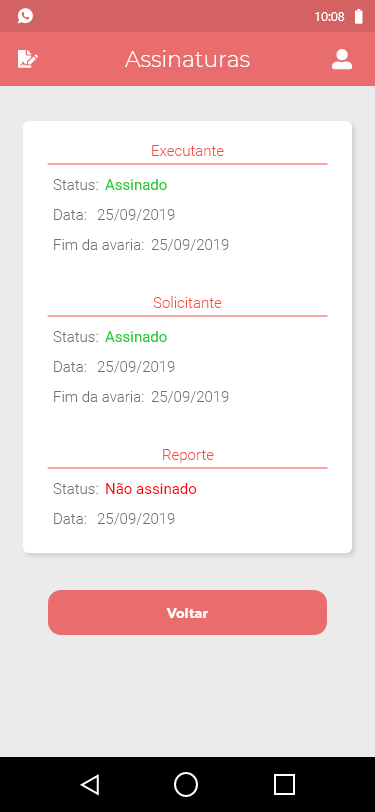
\includegraphics[scale=.65]{Figuras/ASSINATURAS}}
	}
	
\end{figure}

\newpage

Tela de Checklist dos equipamentos de proteção individual.
\begin{figure}[htb]
	\centering
	\mbox{%
		\subfigure[Tela EPI]{\label{EPI}%
			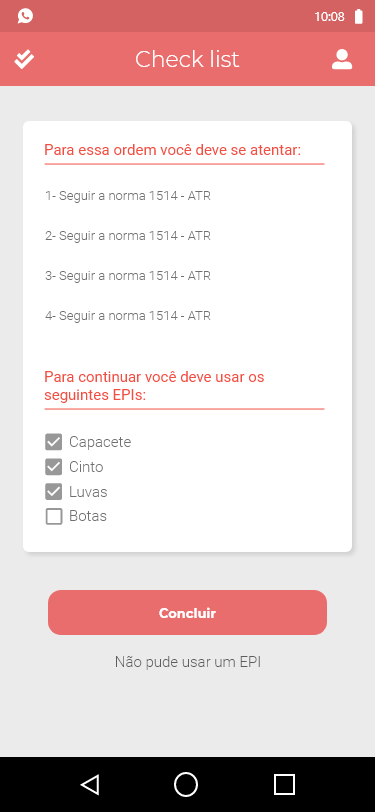
\includegraphics[scale=.65]{Figuras/EPI}}
	}
	
\end{figure}

\newpage

Tela para se justificação do motivo por não utilizar algum EPI especifico.

\begin{figure}[htb]
	\centering
	\mbox{%
		\subfigure[Tela justificação não uso EPI]{\label{EPI_1}%
			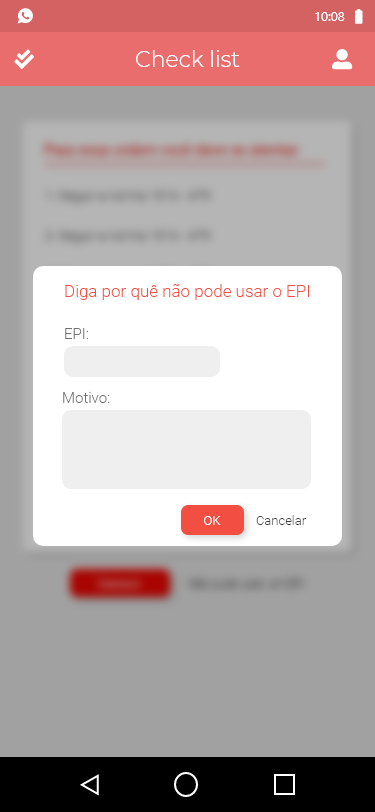
\includegraphics[scale=.65]{Figuras/EPI_1}}\qquad
	}
	
\end{figure}
\newpage
% ---
% ---

\begin{center}
	Protótipos da parte WEB.
\end{center}


Tela para se realizar o login no sistema WEB.

\begin{figure}[H]
	\centering
	\mbox{%
		\subfigure[Tela de login]{\label{LOGIN_1}%
			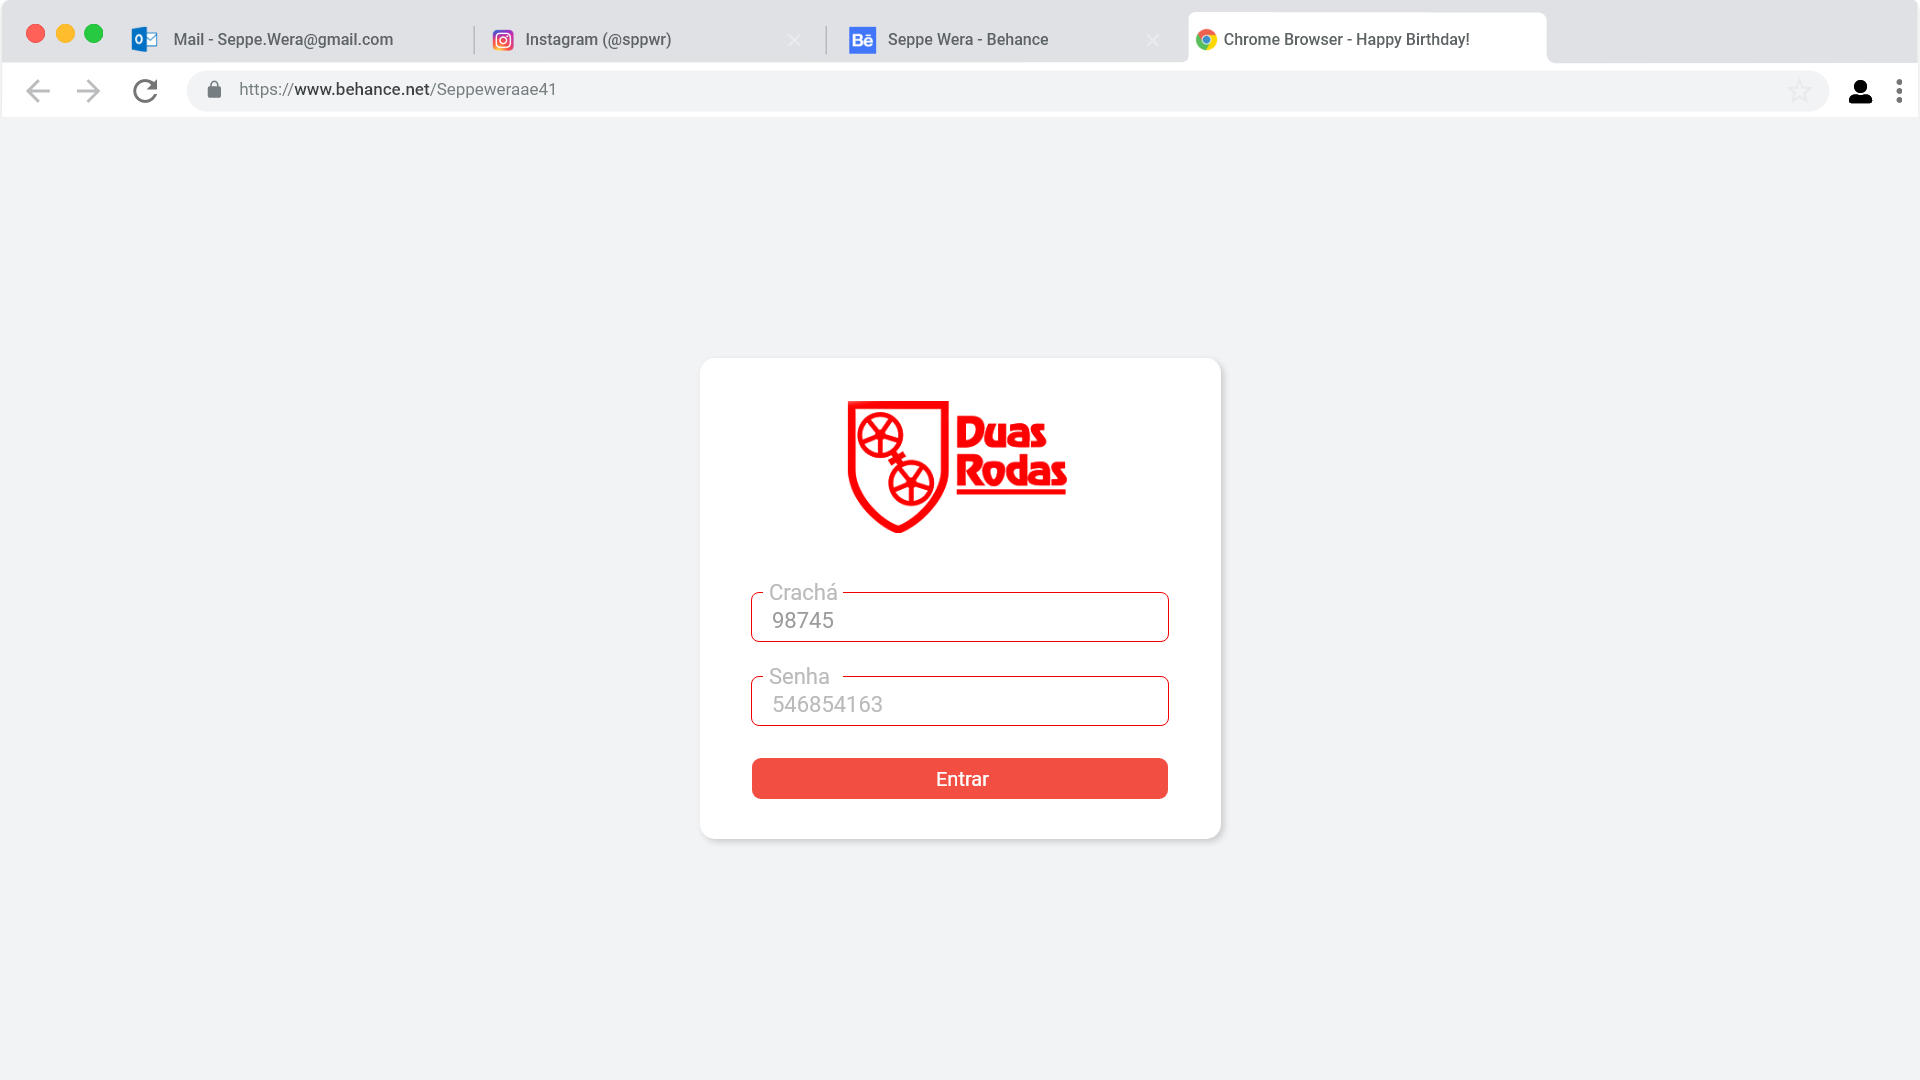
\includegraphics[scale=.32,angle=90]{Figuras/LOGIN_1}}\qquad
	}
	
\end{figure}
\newpage
Tela de dashboard com as peçotes disponíveis no sistema assim como gráficos e relatórios das OS.

\begin{figure}[htb]
	\centering
	\mbox{%
		\subfigure[Tela de dashboard]{\label{DASHBOARD_2}%
			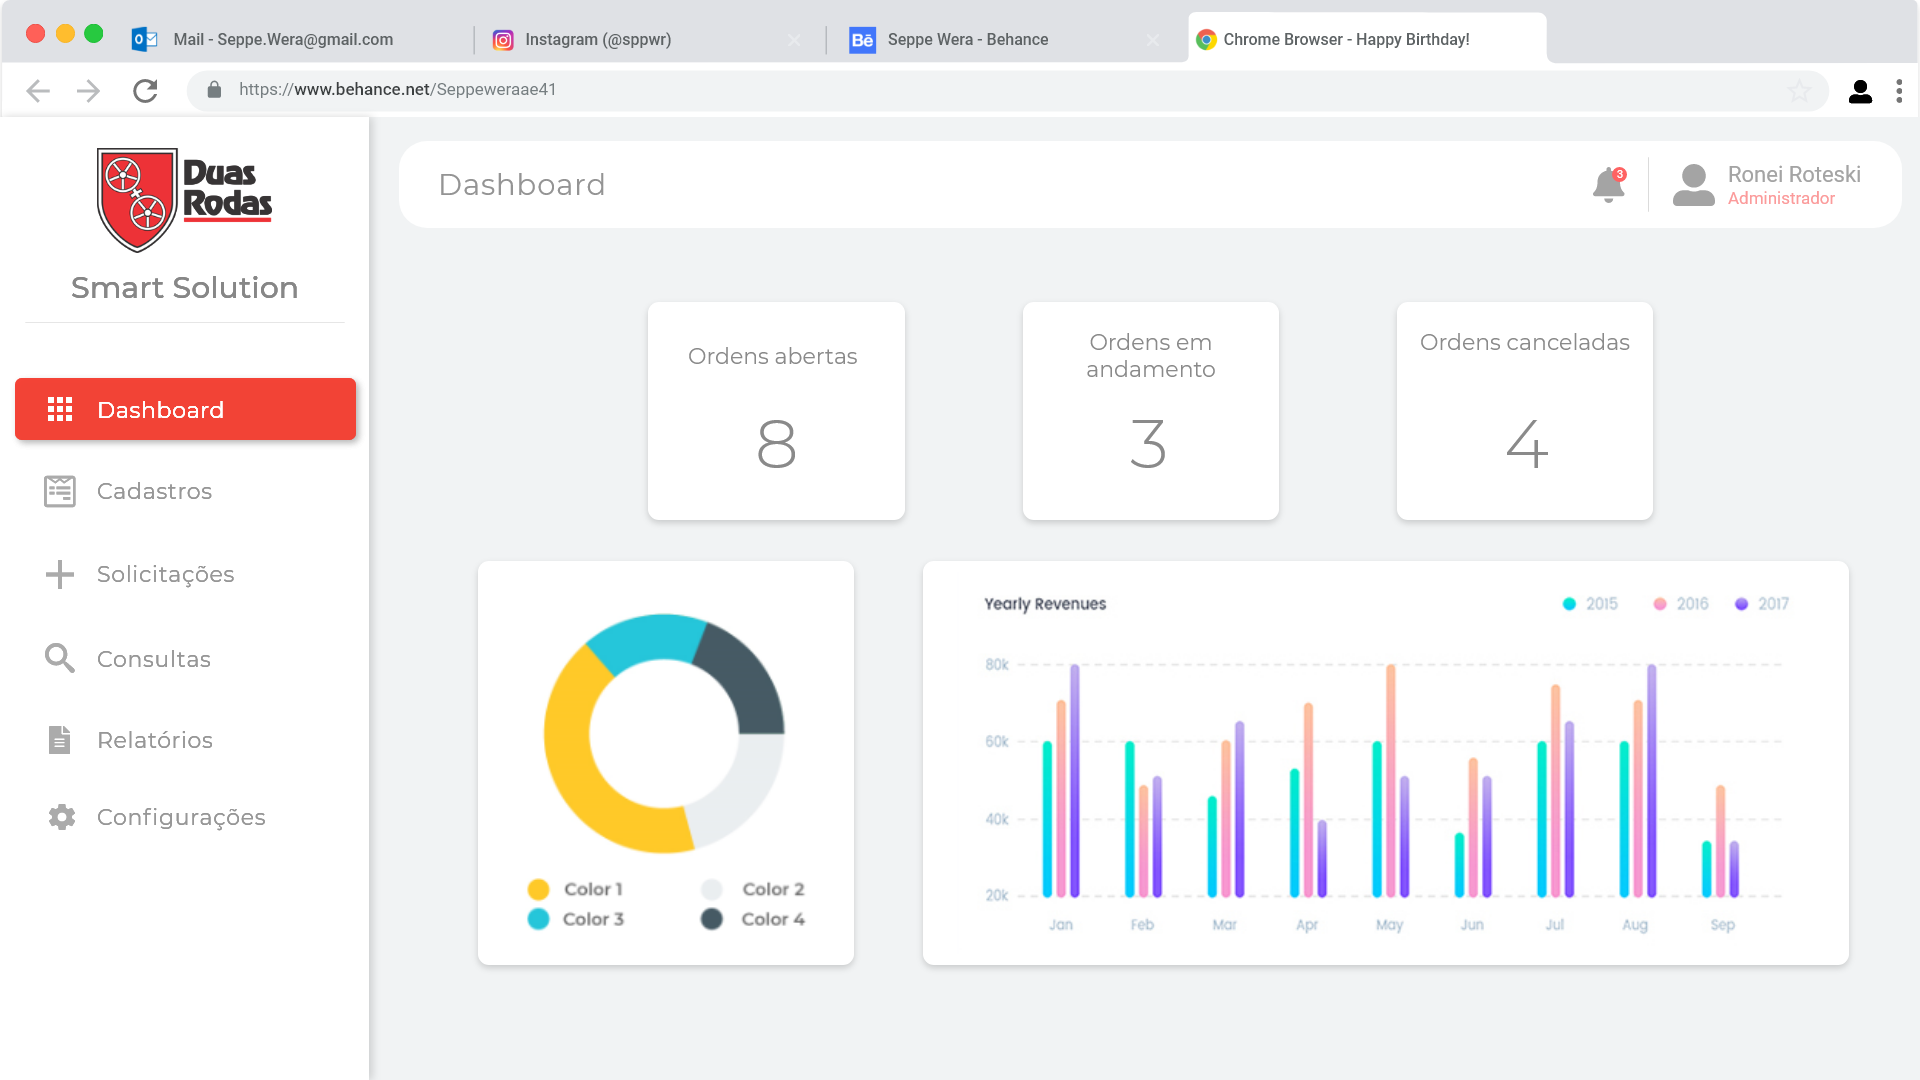
\includegraphics[scale=.32,angle=90]{Figuras/DASHBOARD_2}}\qquad
	}
	
\end{figure}
\newpage

Tela com as opções de cadastramentos disponíveis no sistema.

\begin{figure}[htb]
	\centering
	\mbox{%
		\subfigure[Tela de Cadastramento]{\label{CADASTROS_3}%
			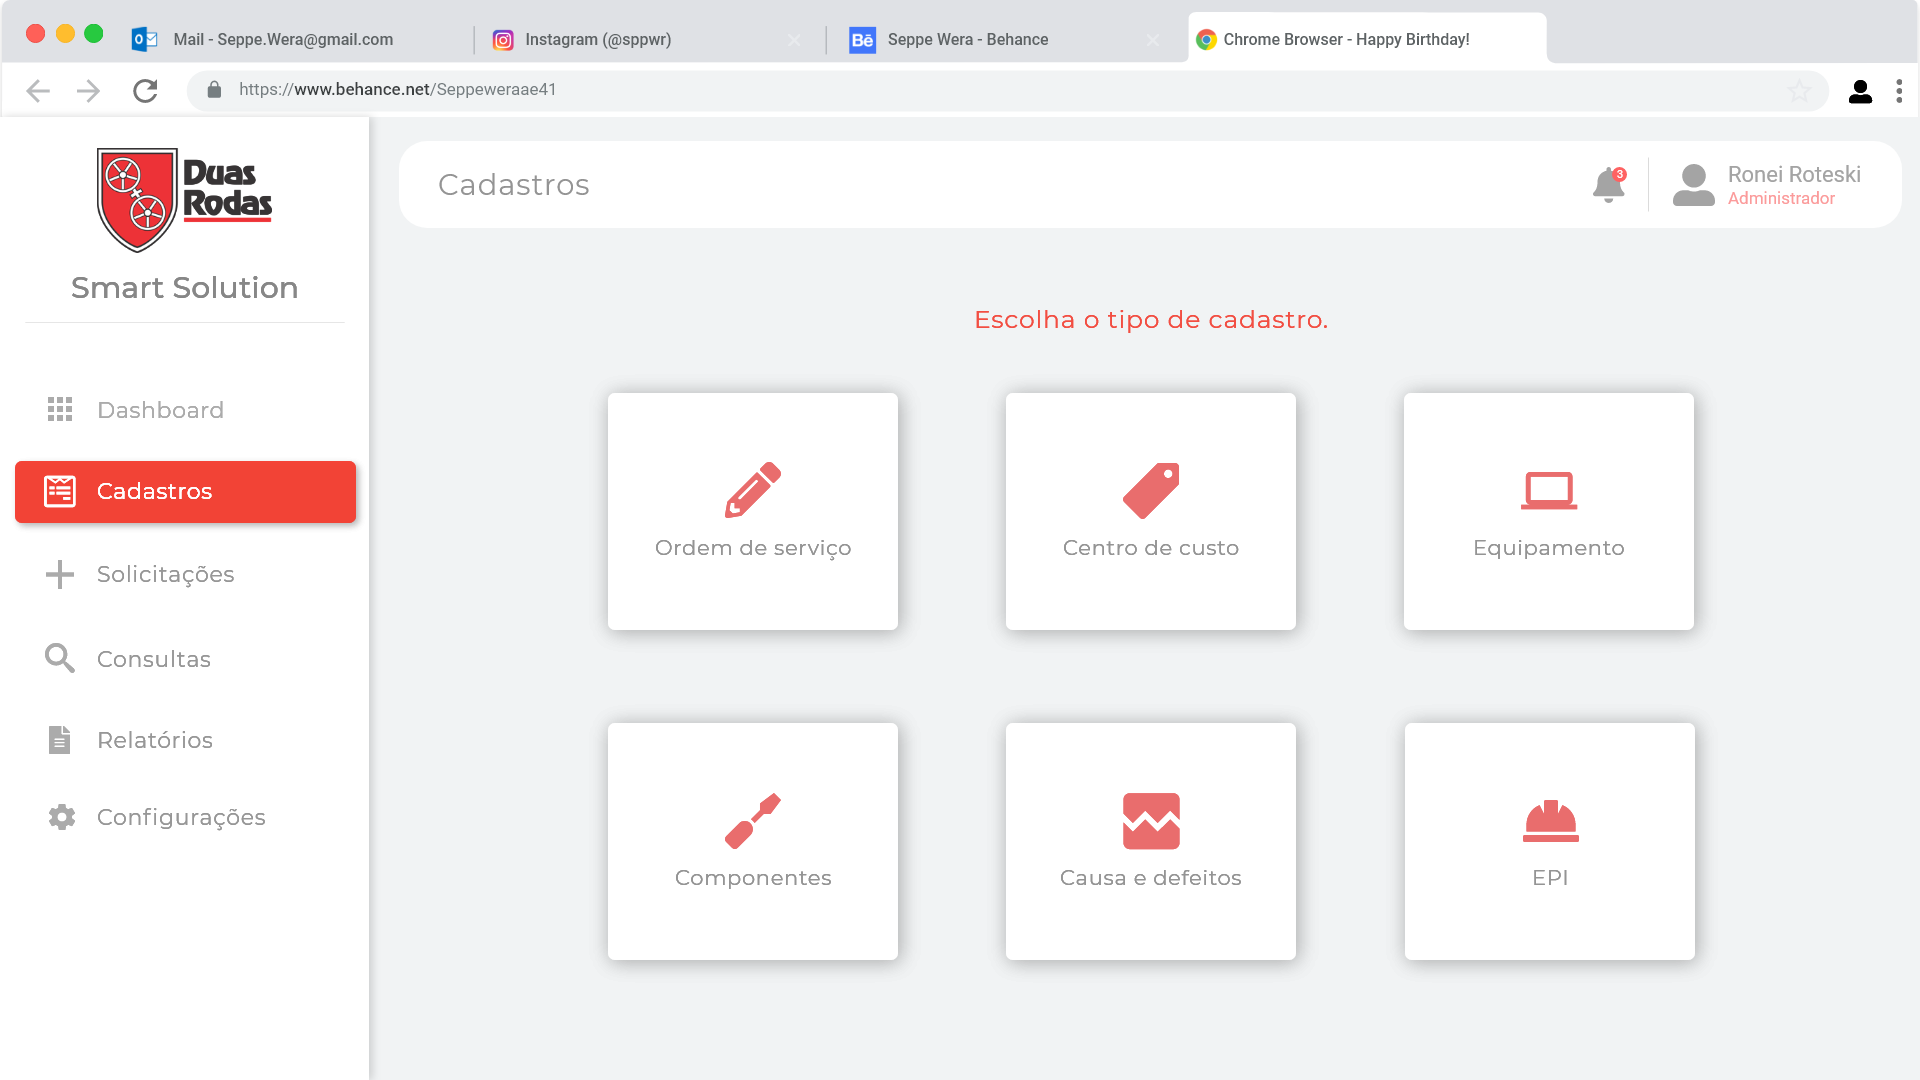
\includegraphics[scale=.32,angle=90]{Figuras/CADASTROS_3}}\qquad
	}
	
\end{figure}
\newpage
Tela para se cadastrar ordem de serviços no sistema de forma manual.

\begin{figure}[htb]
	\centering
	\mbox{%
		\subfigure[Tela cadastro OS]{\label{CADASTRO_OS_4}%
			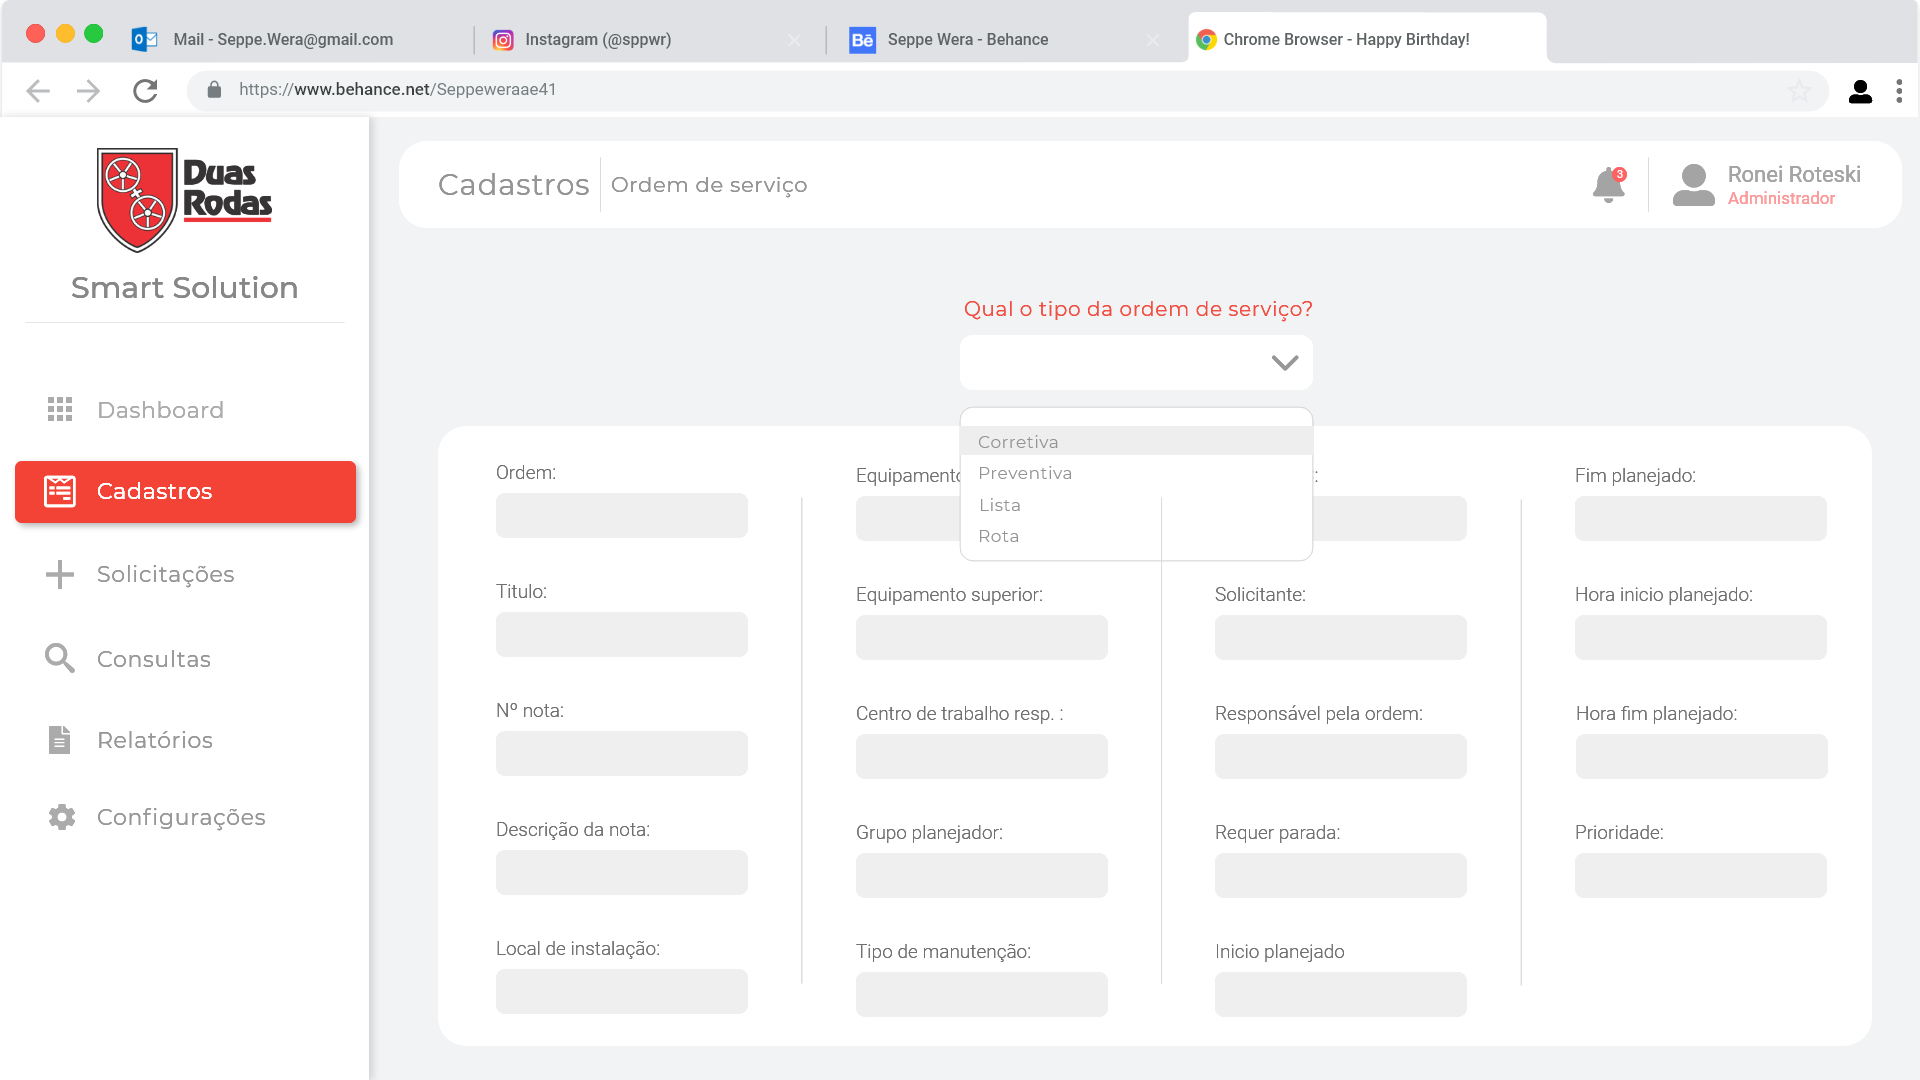
\includegraphics[scale=.32,angle=90]{Figuras/CADASTRO_OS_4}}\qquad
	}
	
\end{figure}
\newpage

Tela para cadastrar equipamentos no sistema.

\begin{figure}[htb]
	\centering
	\mbox{%
		\subfigure[Tela cadastro equipamento]{\label{CADASTRO_EQUIPAMENTO_5}%
			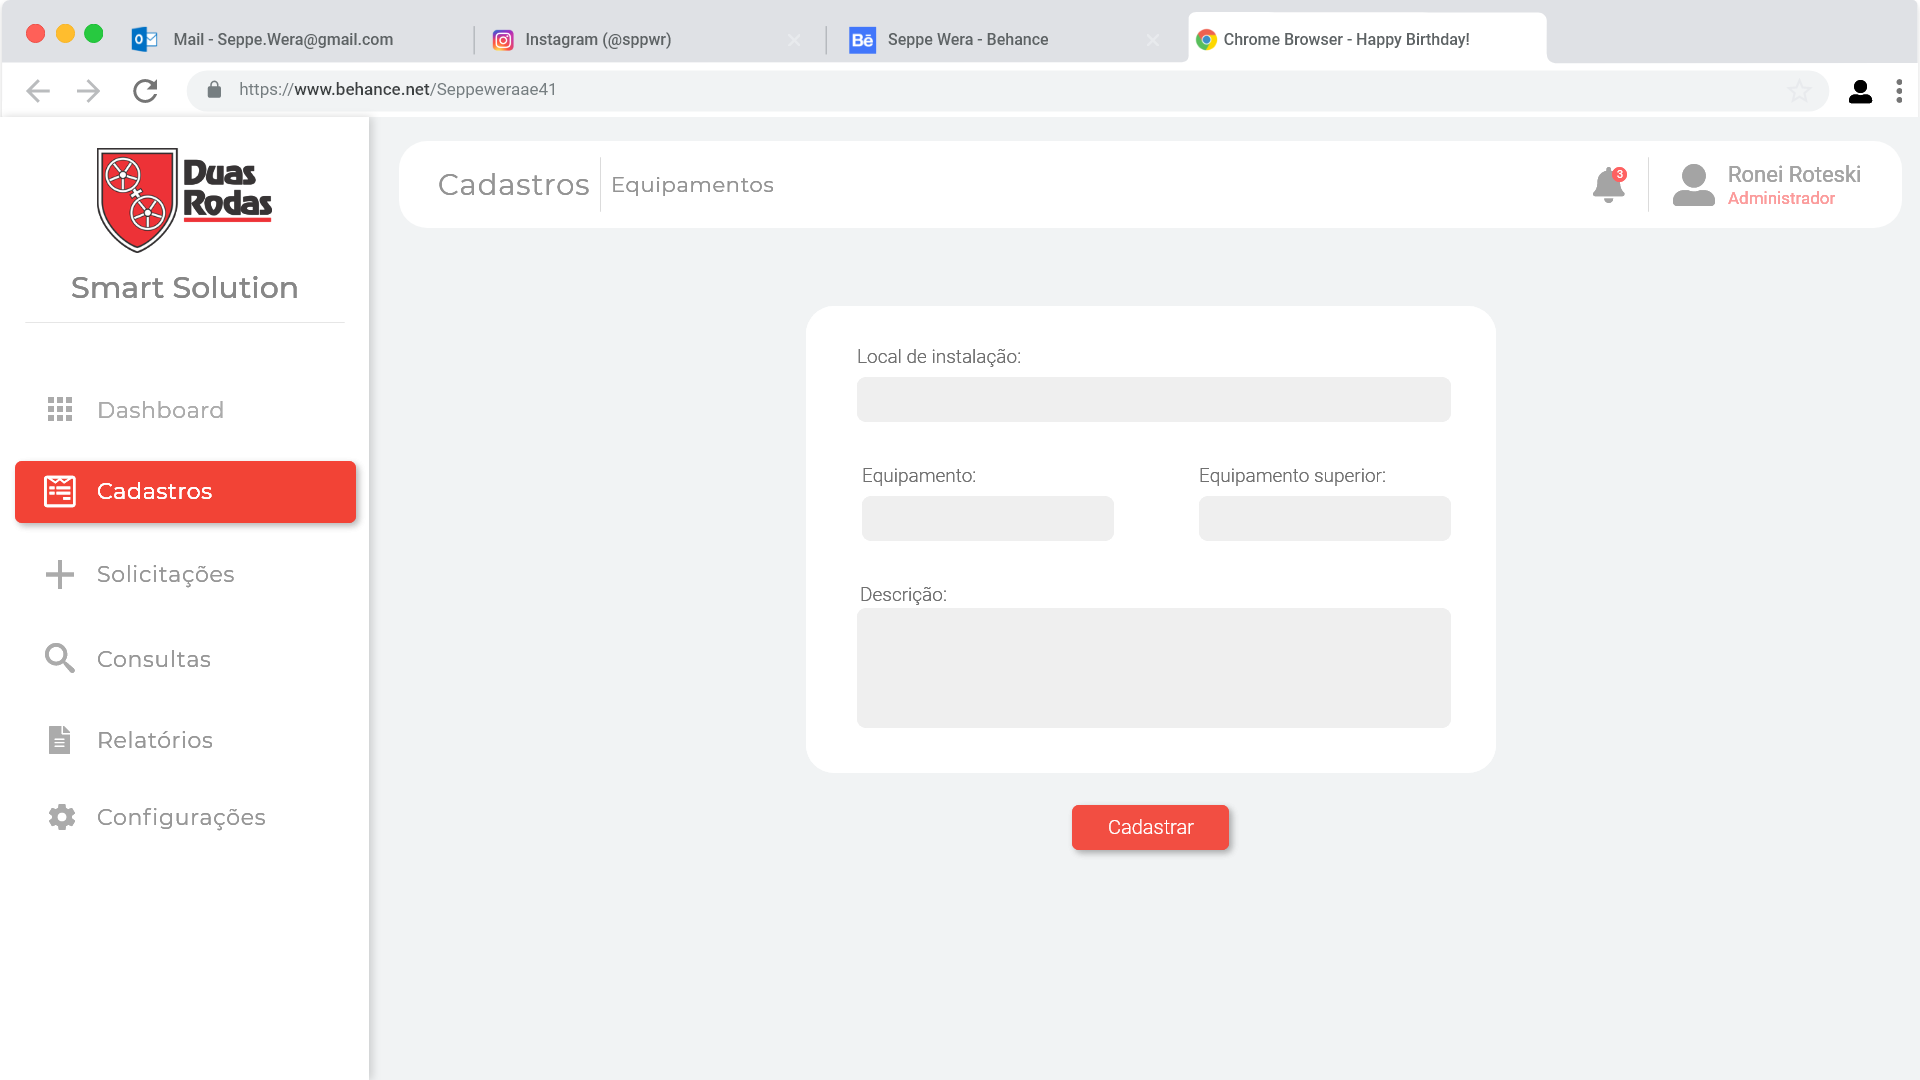
\includegraphics[scale=.32,angle=90]{Figuras/CADASTRO_EQUIPAMENTO_5}}\qquad
	}
	
\end{figure}
\newpage

Tela para cadastrar componentes de cada maquina.

\begin{figure}[htb]
	\centering
	\mbox{%
		\subfigure[Tela de cadastros de componentes]{\label{CADASTRO_COMPONENTE_6}%
			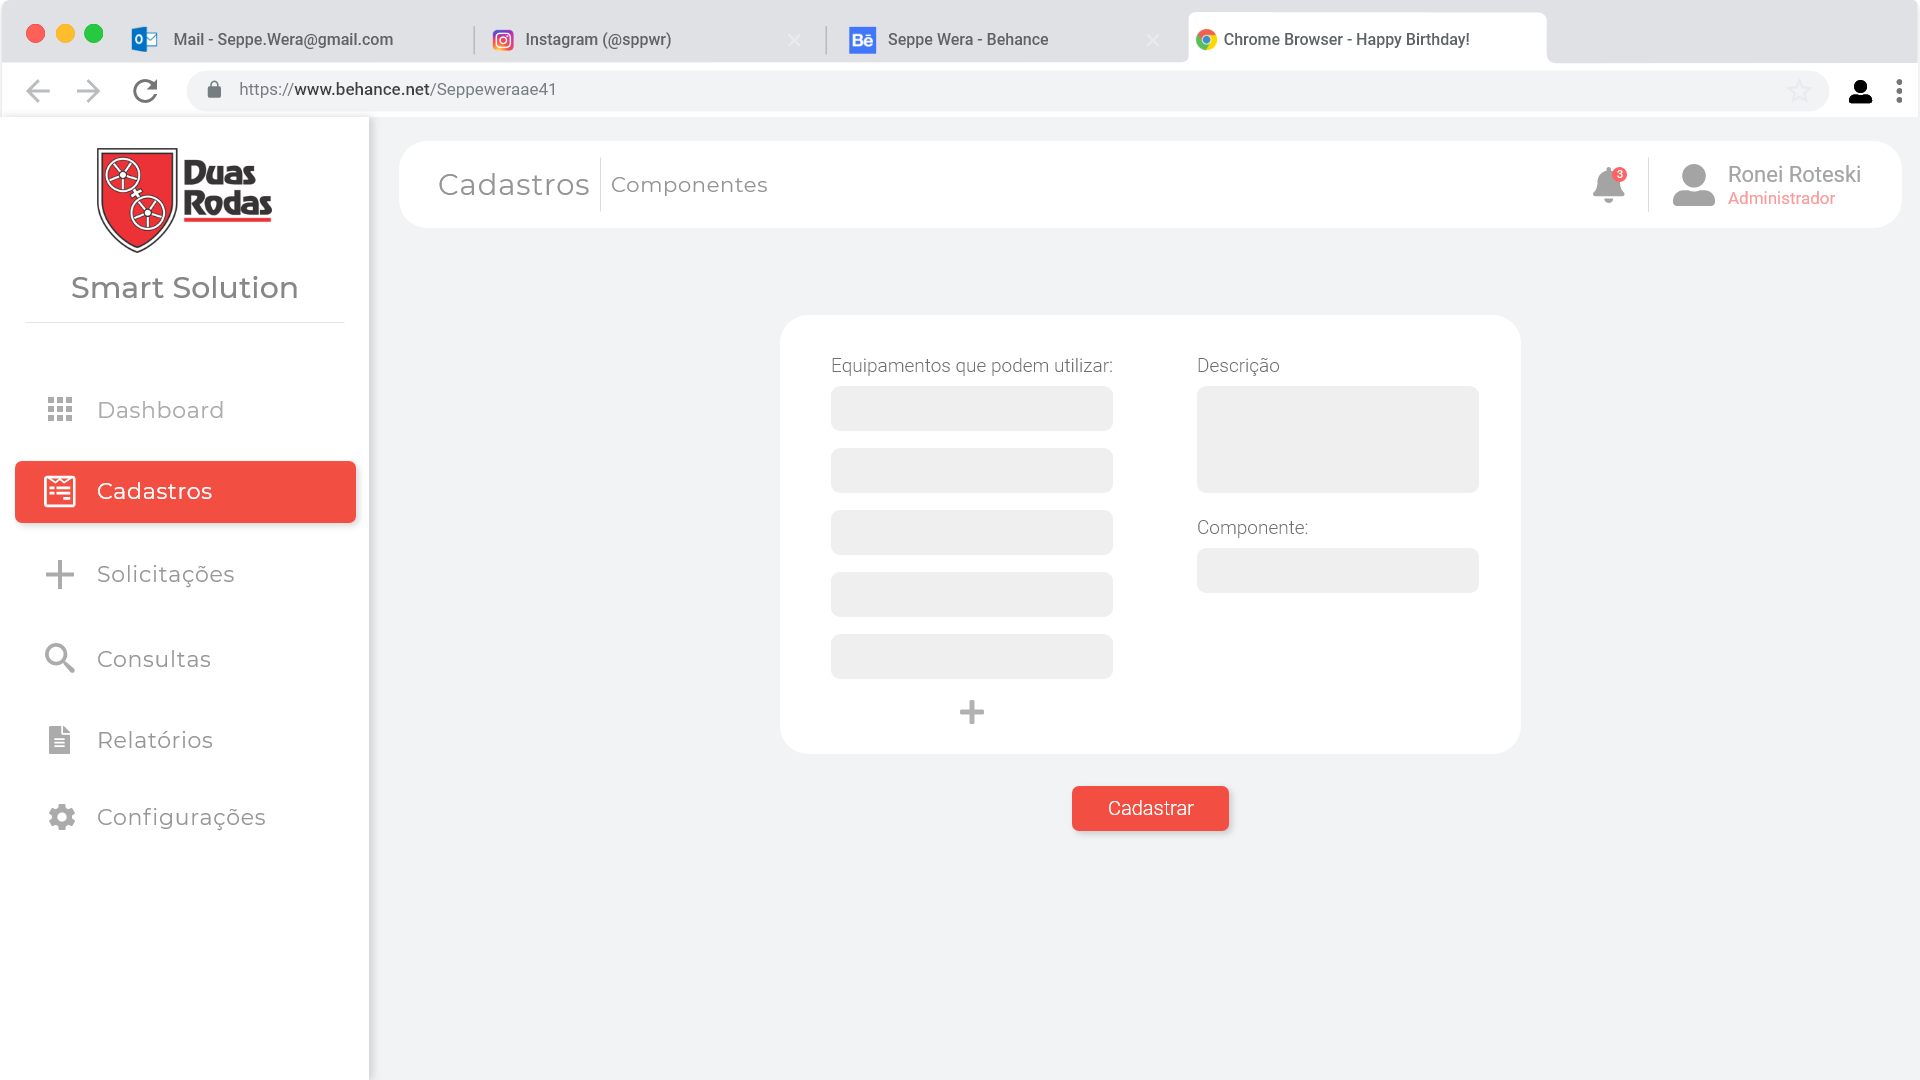
\includegraphics[scale=.32,angle=90]{Figuras/CADASTRO_COMPONENTE_6}}\qquad
	}
	
\end{figure}

\newpage

Tela com finalidade de cadastrar EPI.

\begin{figure}[htb]
	\centering
	\mbox{%
		\subfigure[Tela cadastro EPI]{\label{CADASTRO_EPI_7}%
			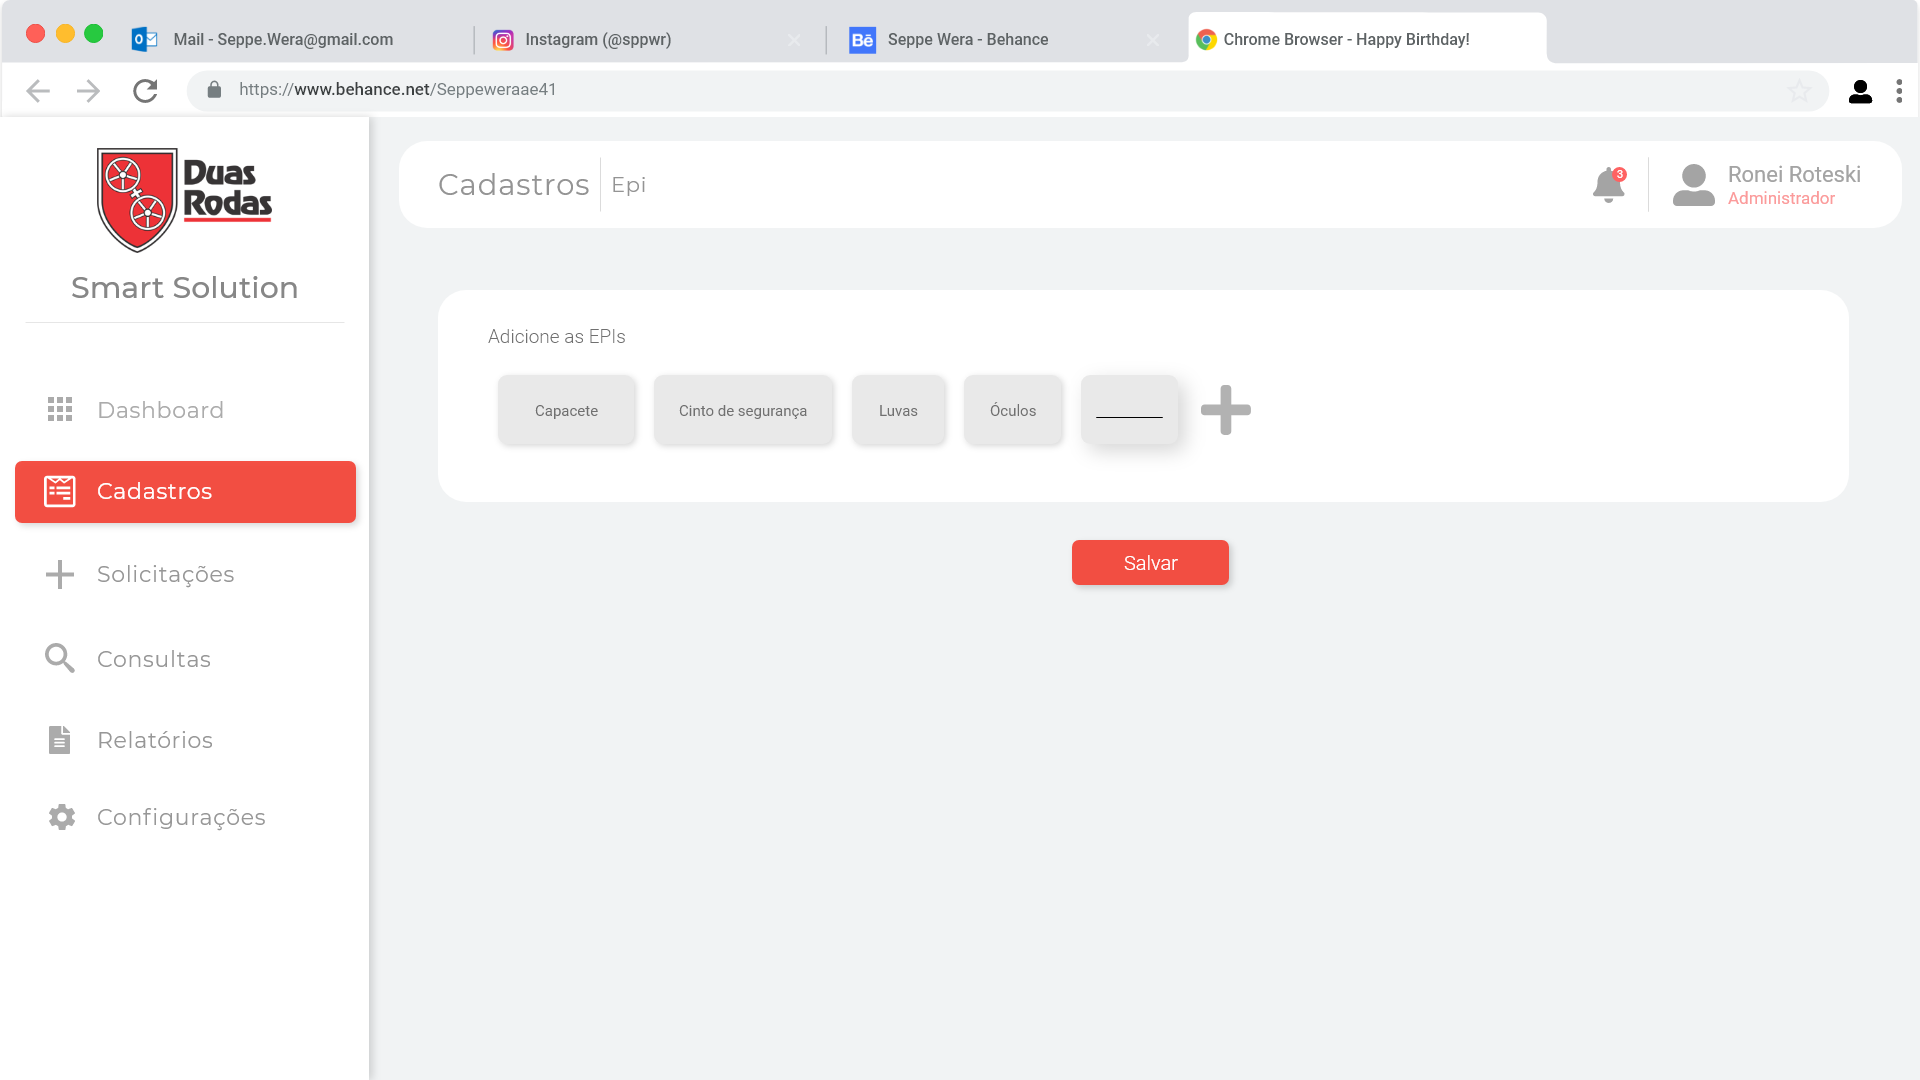
\includegraphics[scale=.32,angle=90]{Figuras/CADASTRO_EPI_7}}\qquad
	}
	
\end{figure}
\newpage
Tela para cadastrar causas e sintomas que ja ocorrerão ou novos.

\begin{figure}[htb]
	\centering
	\mbox{%
		\subfigure[Tela cadastro causas e sintomas]{\label{CADASTRO_causa_8}%
			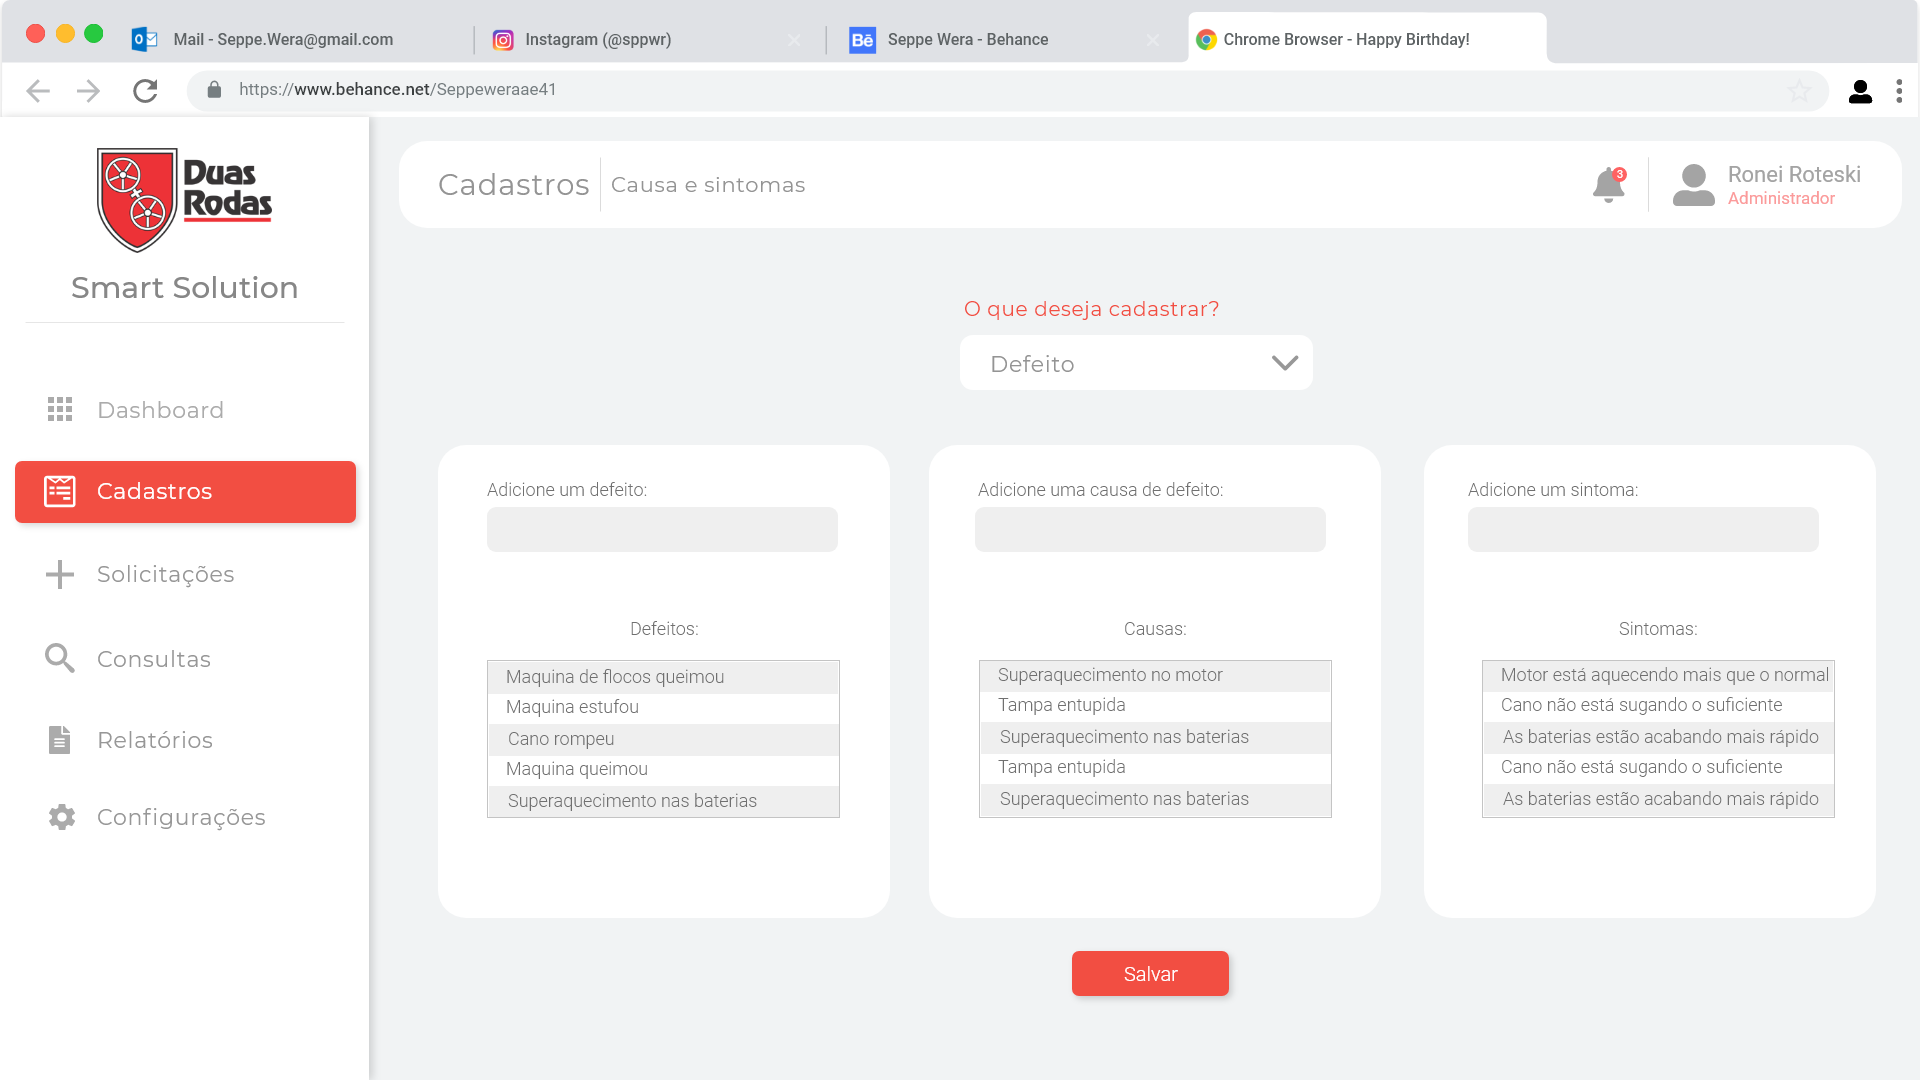
\includegraphics[scale=.32,angle=90]{Figuras/CADASTRO_causa_8}}\qquad
	}
	
\end{figure}
\newpage
Tela para cadastrar operações realizadas com lista disponível para evitar duplicar o mesmo procedimentos.

\begin{figure}[htb]
	\centering
	\mbox{%
		\subfigure[Tela cadastro de operações]{\label{CADASTRO_DE_OPERACOES_9}%
			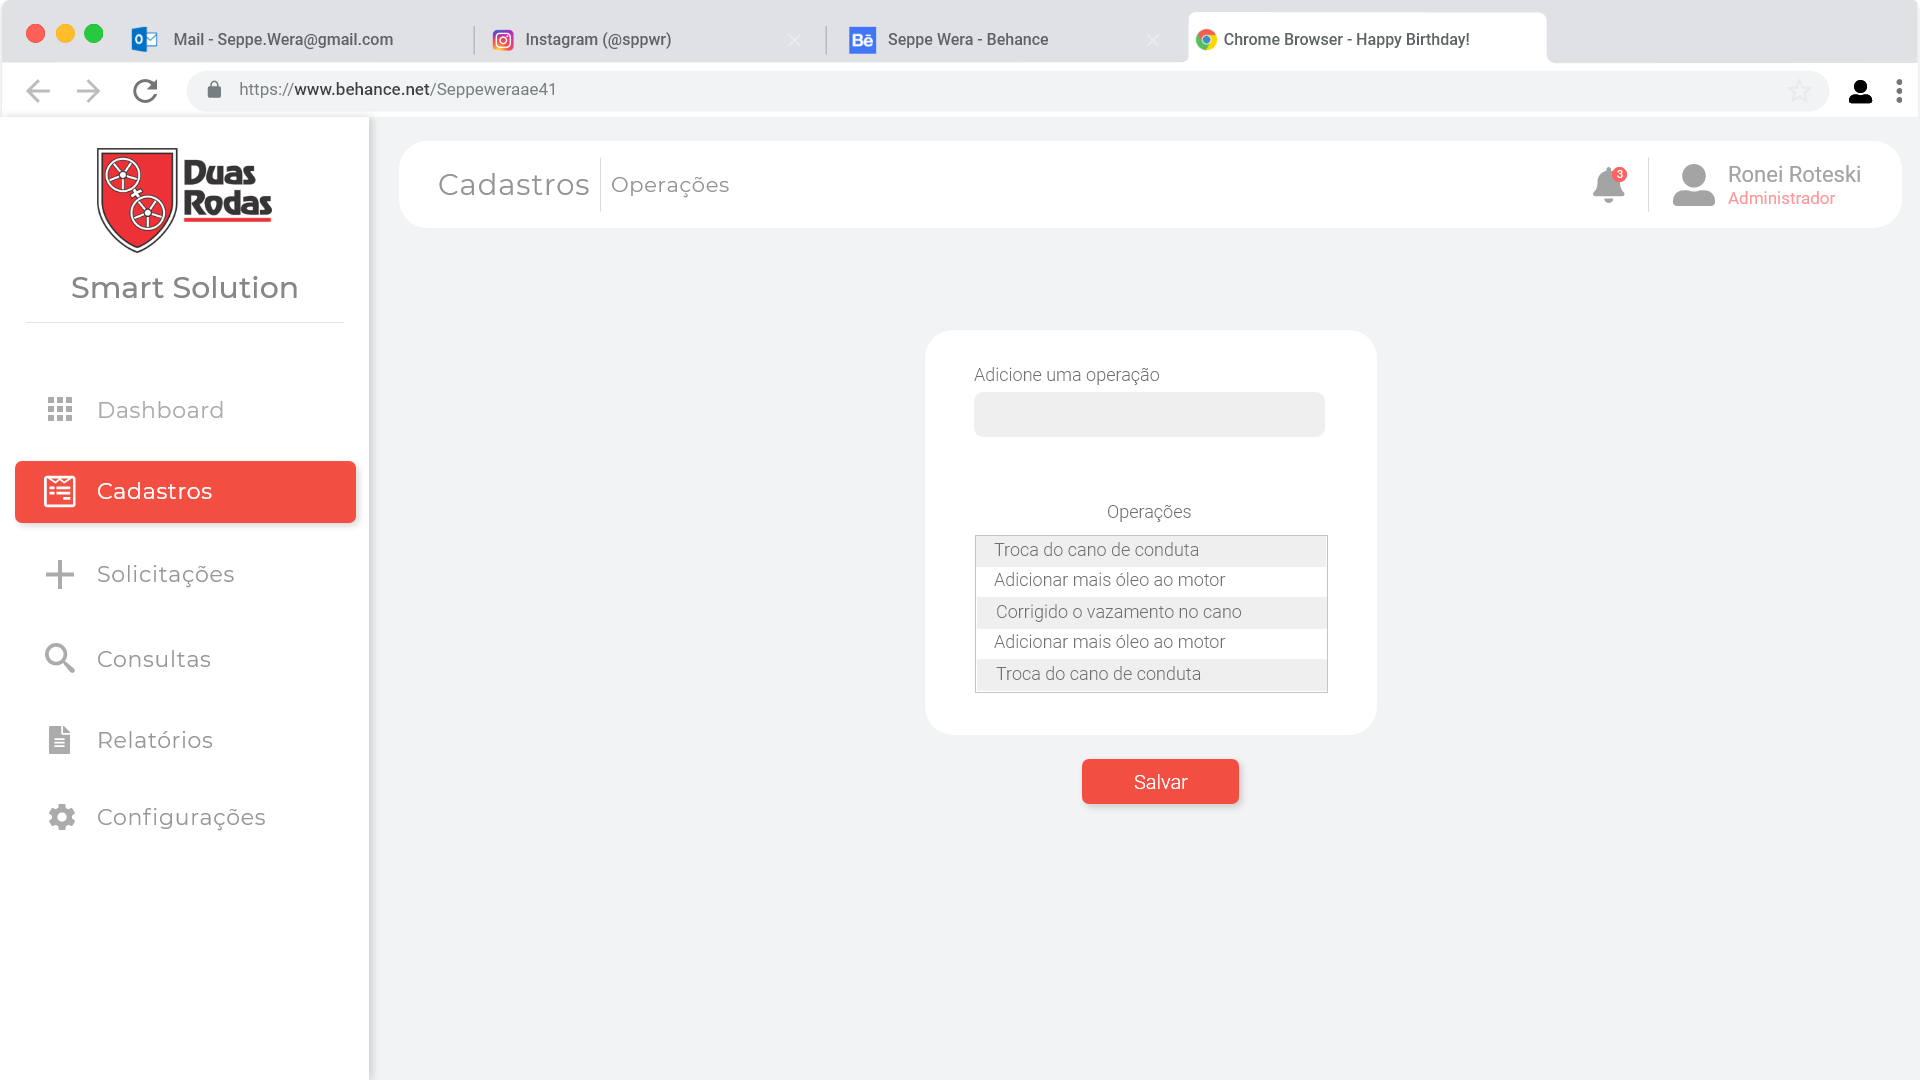
\includegraphics[scale=.32,angle=90]{Figuras/CADASTRO_DE_OPERACOES_9}}\qquad
	}
	
\end{figure}
\newpage
Tela para para se solicitar peças para OS previamente ou apos iniciar-se a ordem de serviço. 

\begin{figure}[htb]
	\centering
	\mbox{%
		\subfigure[Tela para solicitar peças]{\label{Solicitacao_10}%
			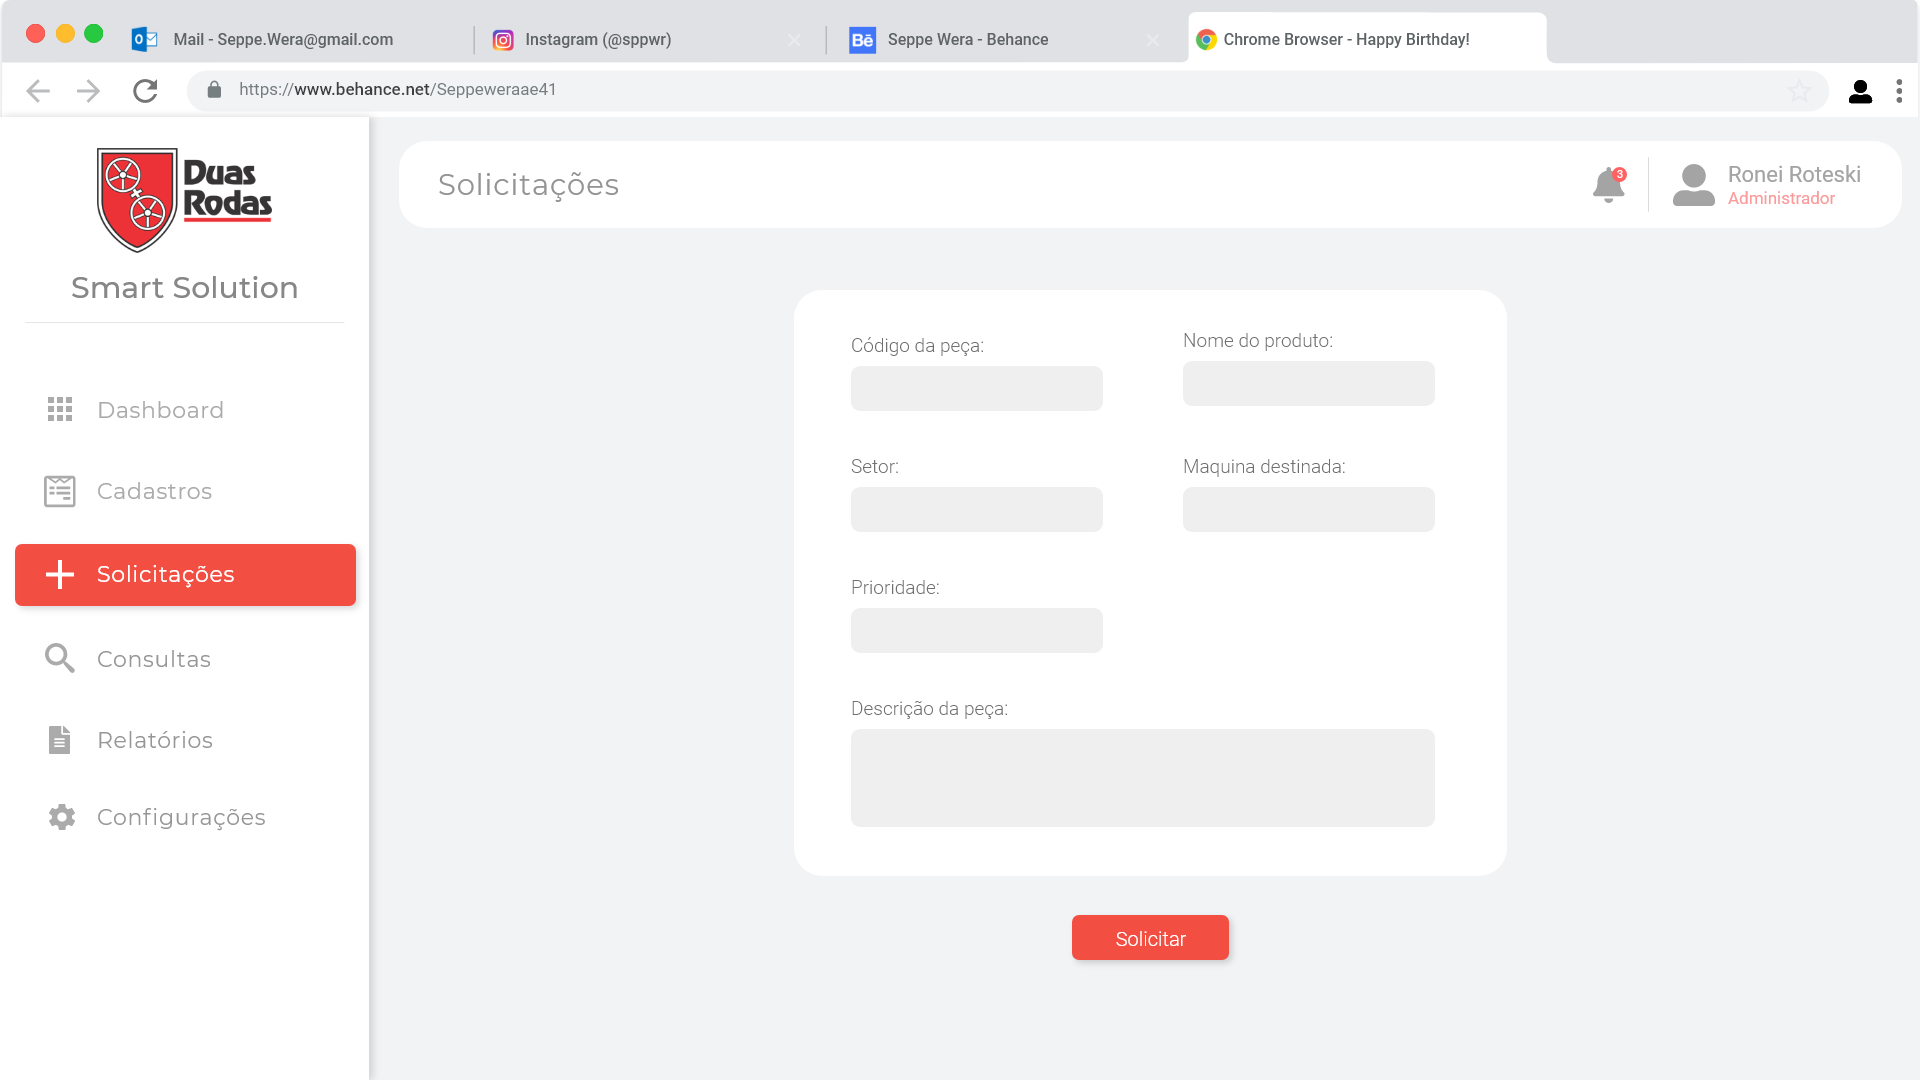
\includegraphics[scale=.32,angle=90]{Figuras/Solicitacao_10}}\qquad
	}
	
\end{figure}
\newpage
Tela de consultar de ordens de serviço com filtros por data ,prioridade, status ou suas próprias em minhas os na parte web.

\begin{figure}[htb]
	\centering
	\mbox{%
		\subfigure[Tela consulta OS]{\label{CONSULTA_11}%
			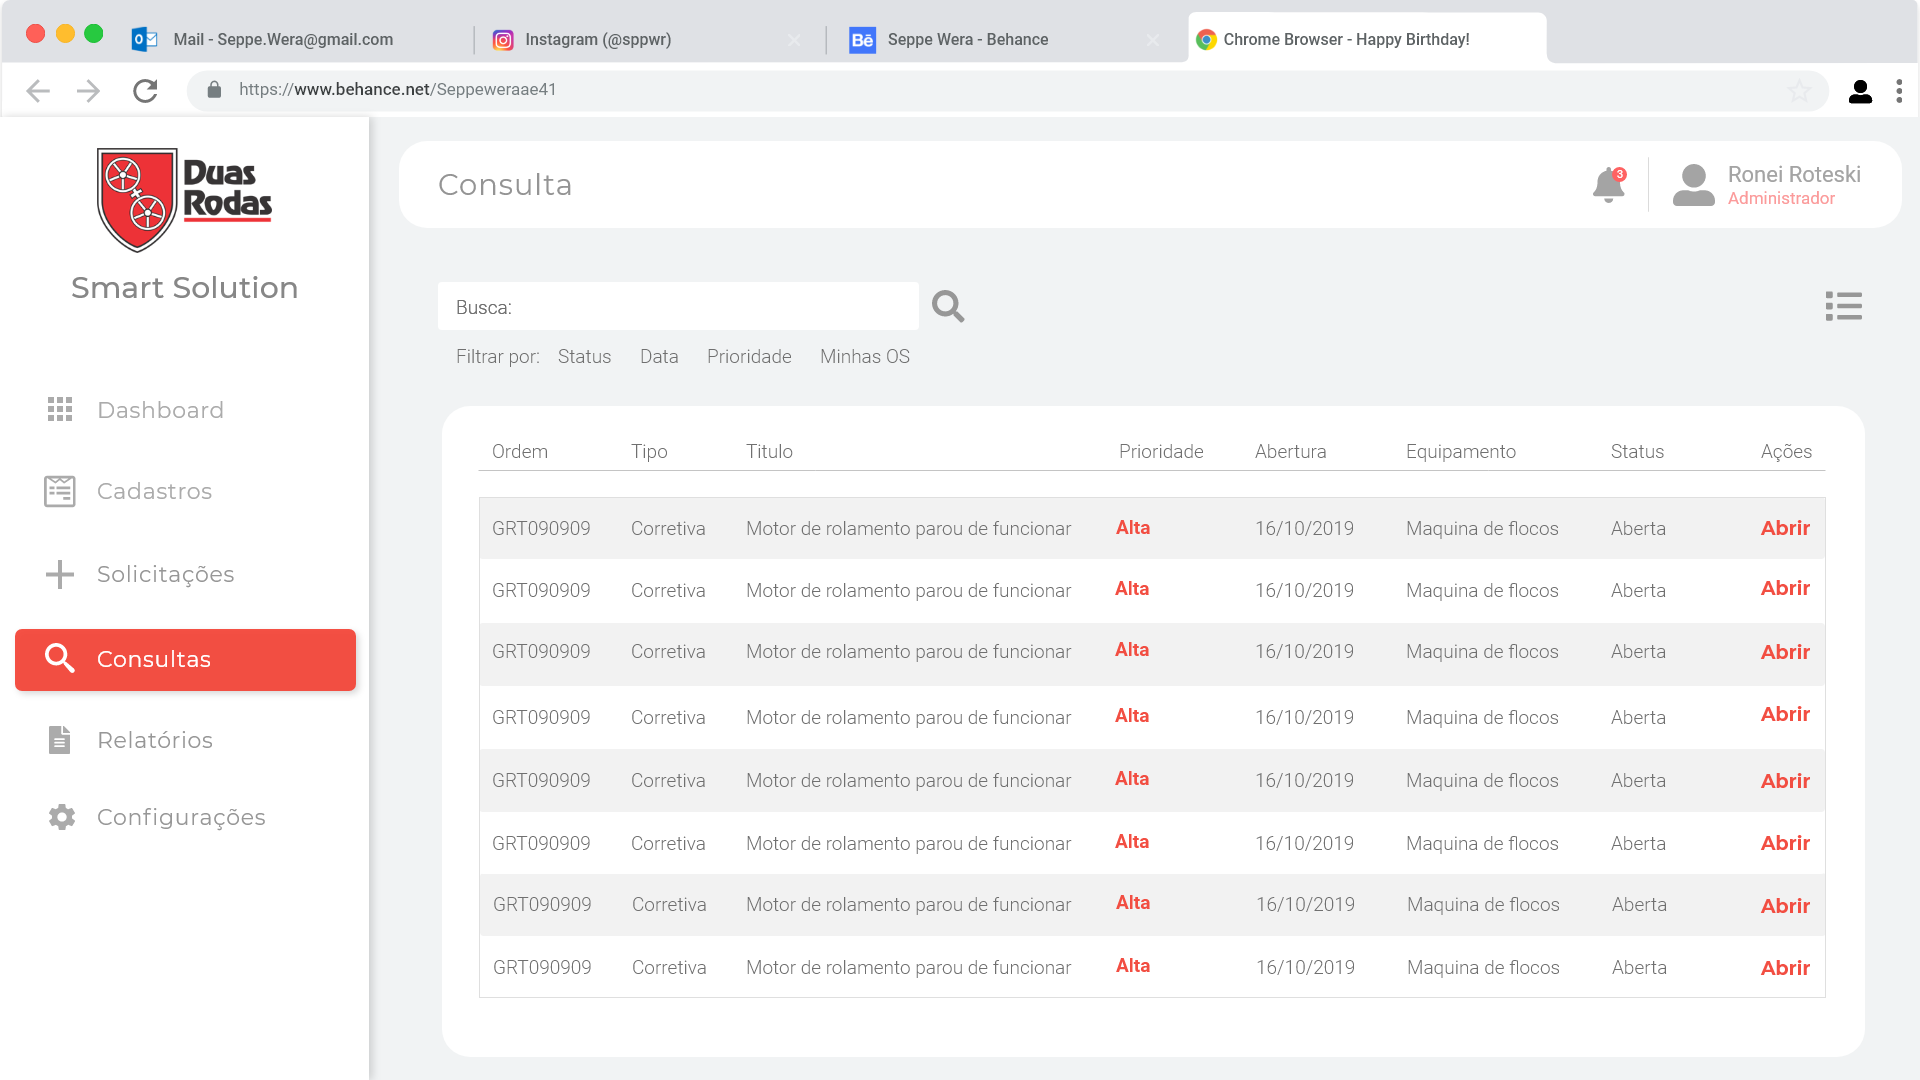
\includegraphics[scale=.32,angle=90]{Figuras/CONSULTA_11}}\qquad
	}
	
\end{figure}
\newpage
Tela de detalhamento de ordem de serviço, com todos as informações da OS e suas opções disponíveis.

\begin{figure}[htb]
	\centering
	\mbox{%
		\subfigure[Tela detalhamento OS]{\label{DETALHAMENTO_12}%
			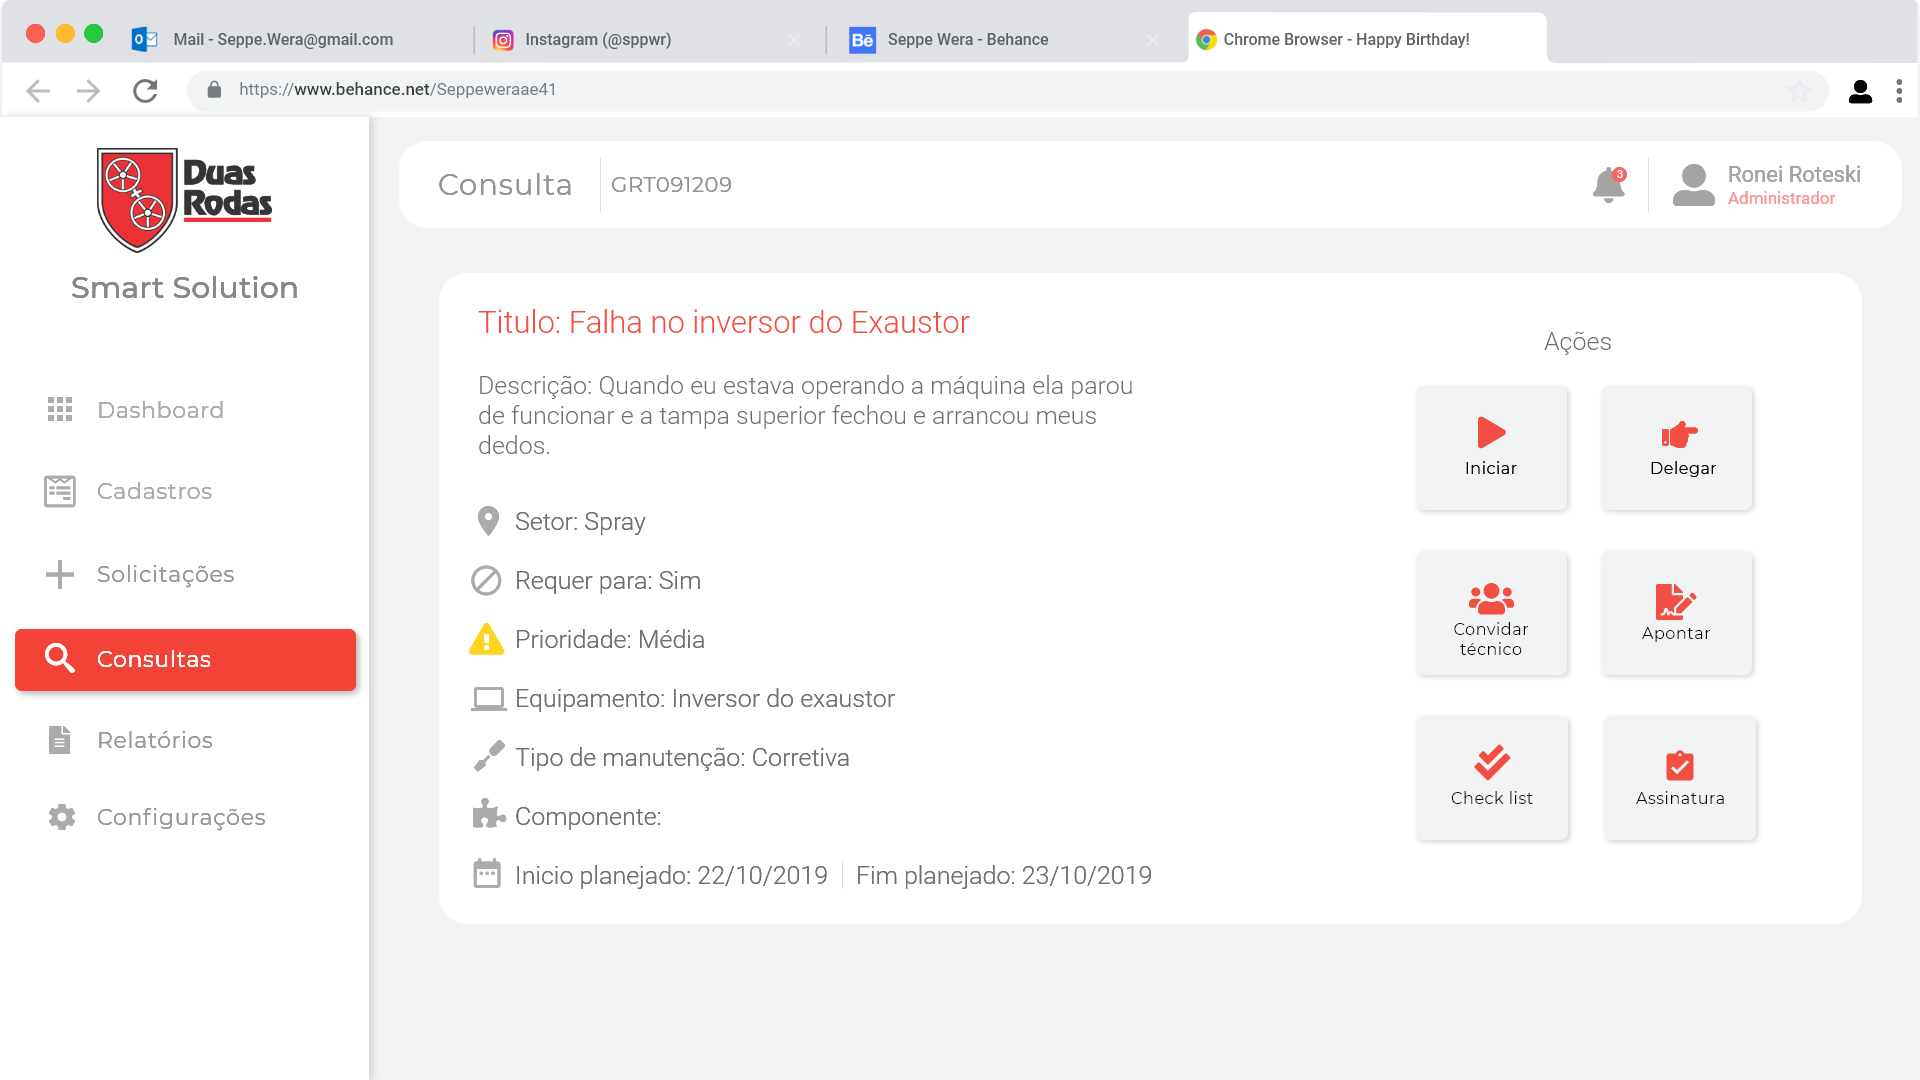
\includegraphics[scale=.32,angle=90]{Figuras/DETALHAMENTO_12}}\qquad
	}
	
\end{figure}
\newpage
Tela de verificação, se o conserto foi concluído.

\begin{figure}[htb]
	\centering
	\mbox{%
		\subfigure[Tela de verificação]{\label{Verificacao_web}%
			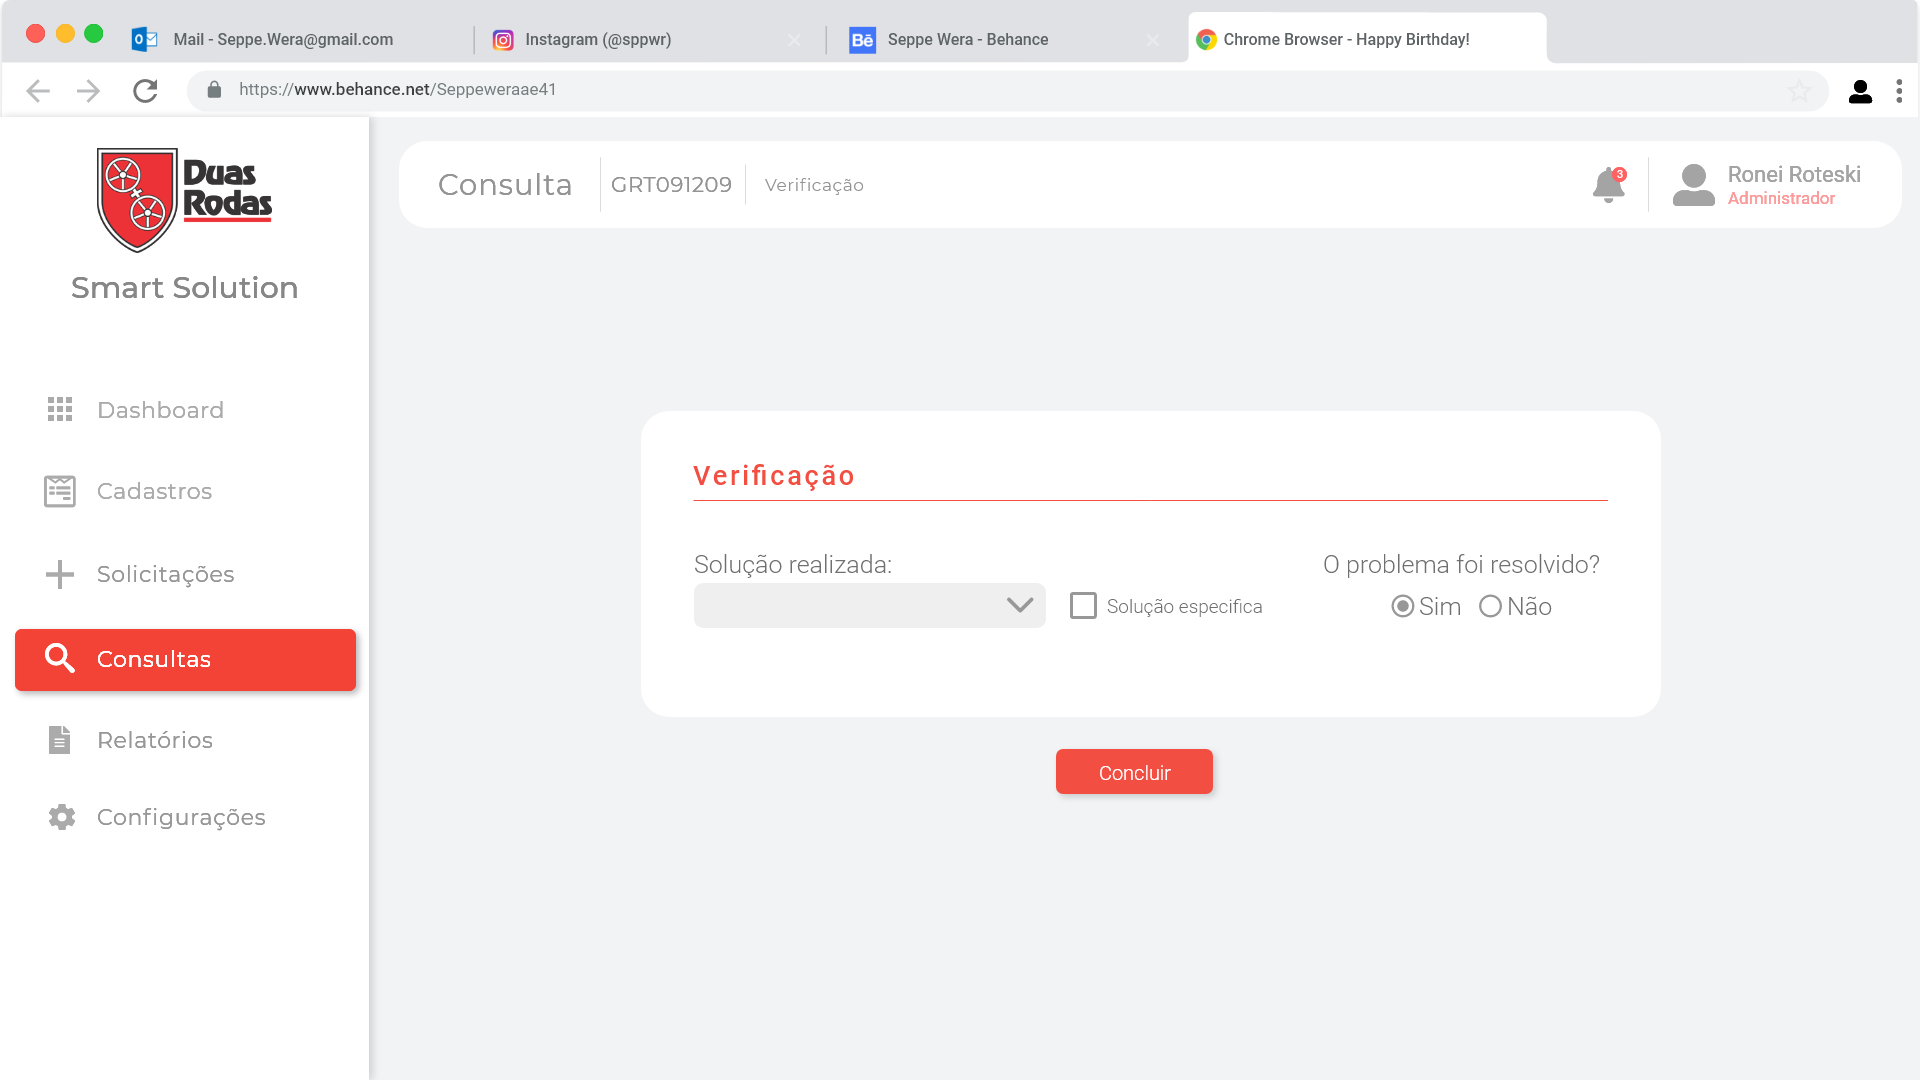
\includegraphics[scale=.32,angle=90]{Figuras/Verificacao_web}}\qquad
	}
	
\end{figure}
\newpage

Tela para apontar horas trabalhadas.
\begin{figure}[htb]
	\centering
	\mbox{%
		\subfigure[Tela de Apontamento]{\label{APONTAMENTO_web}%
			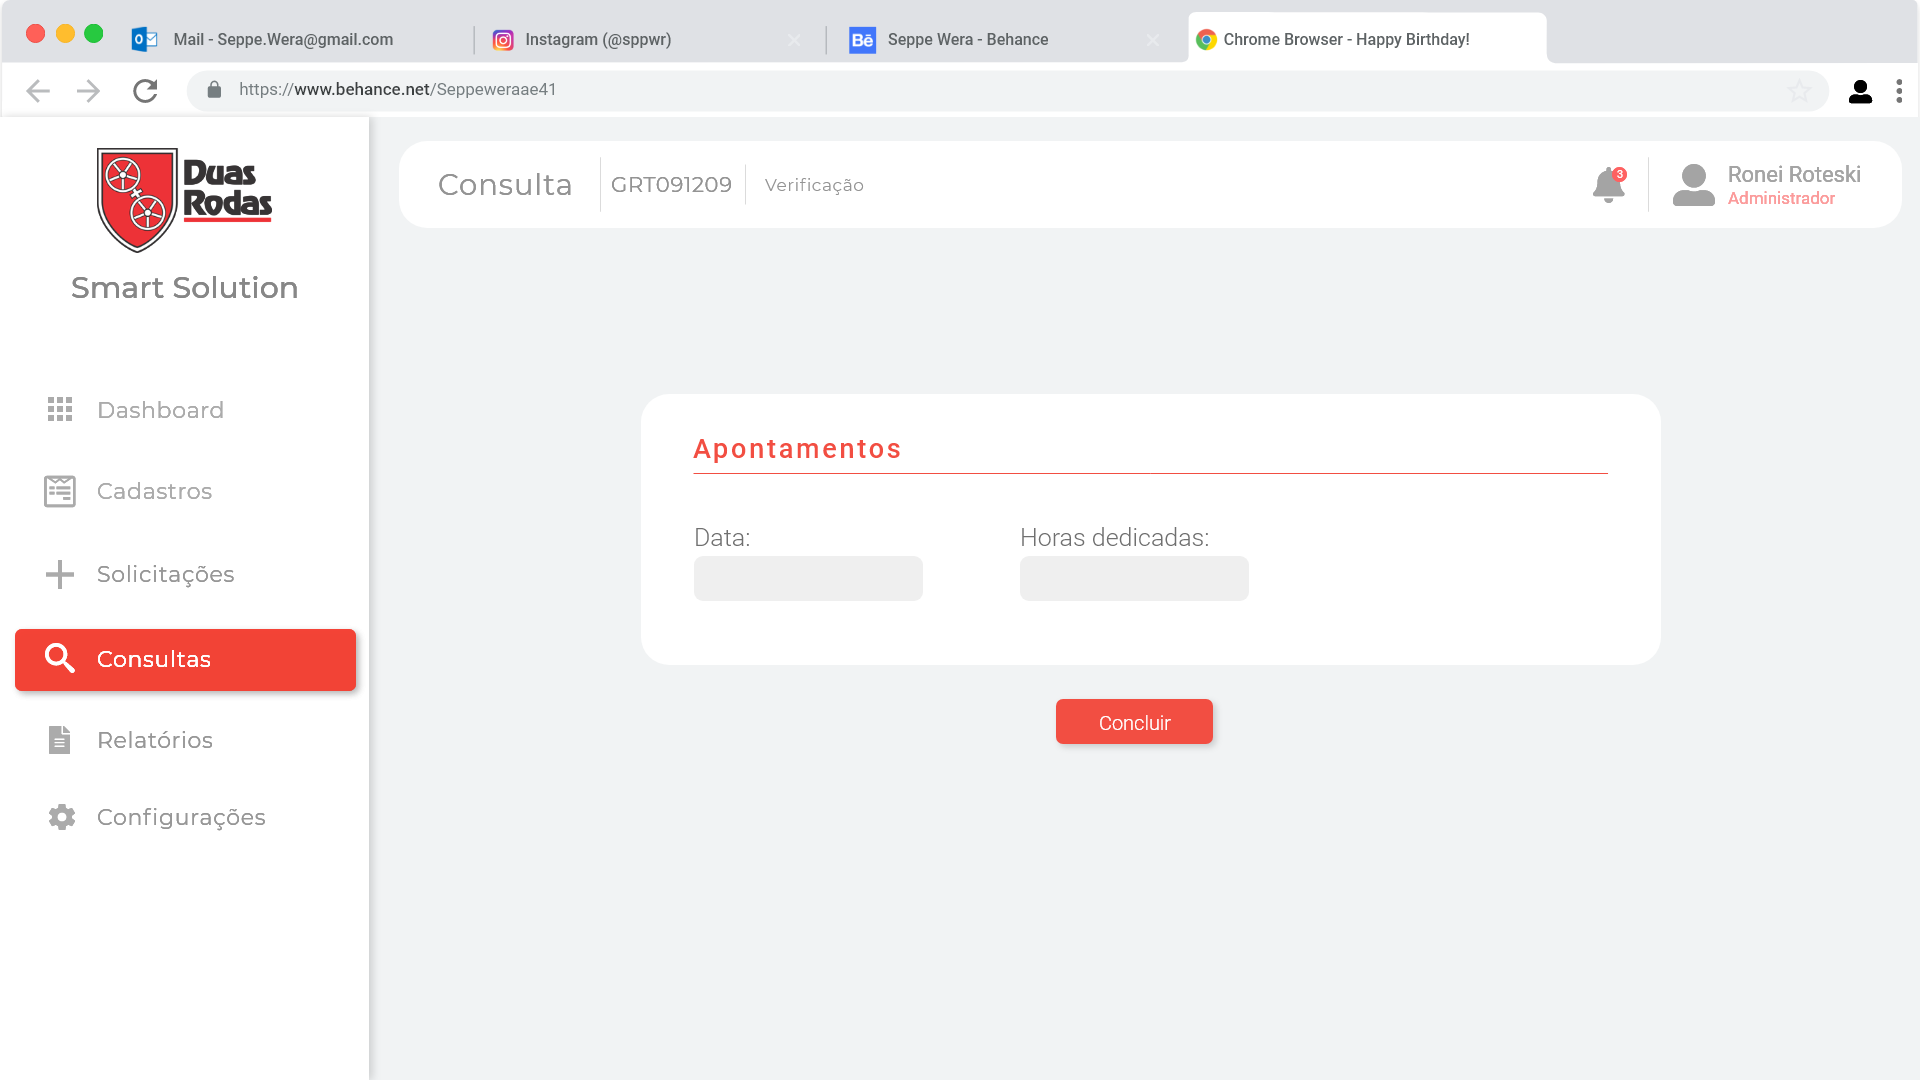
\includegraphics[scale=.32,angle=90]{Figuras/APONTAMENTO_web}}\qquad
	}
	
\end{figure}
\newpage
Tela para verificar se possui todas as assinaturas.
\begin{figure}[htb]
	\centering
	\mbox{%
		\subfigure[Tela de Assinatura]{\label{Assinatura_web}%
			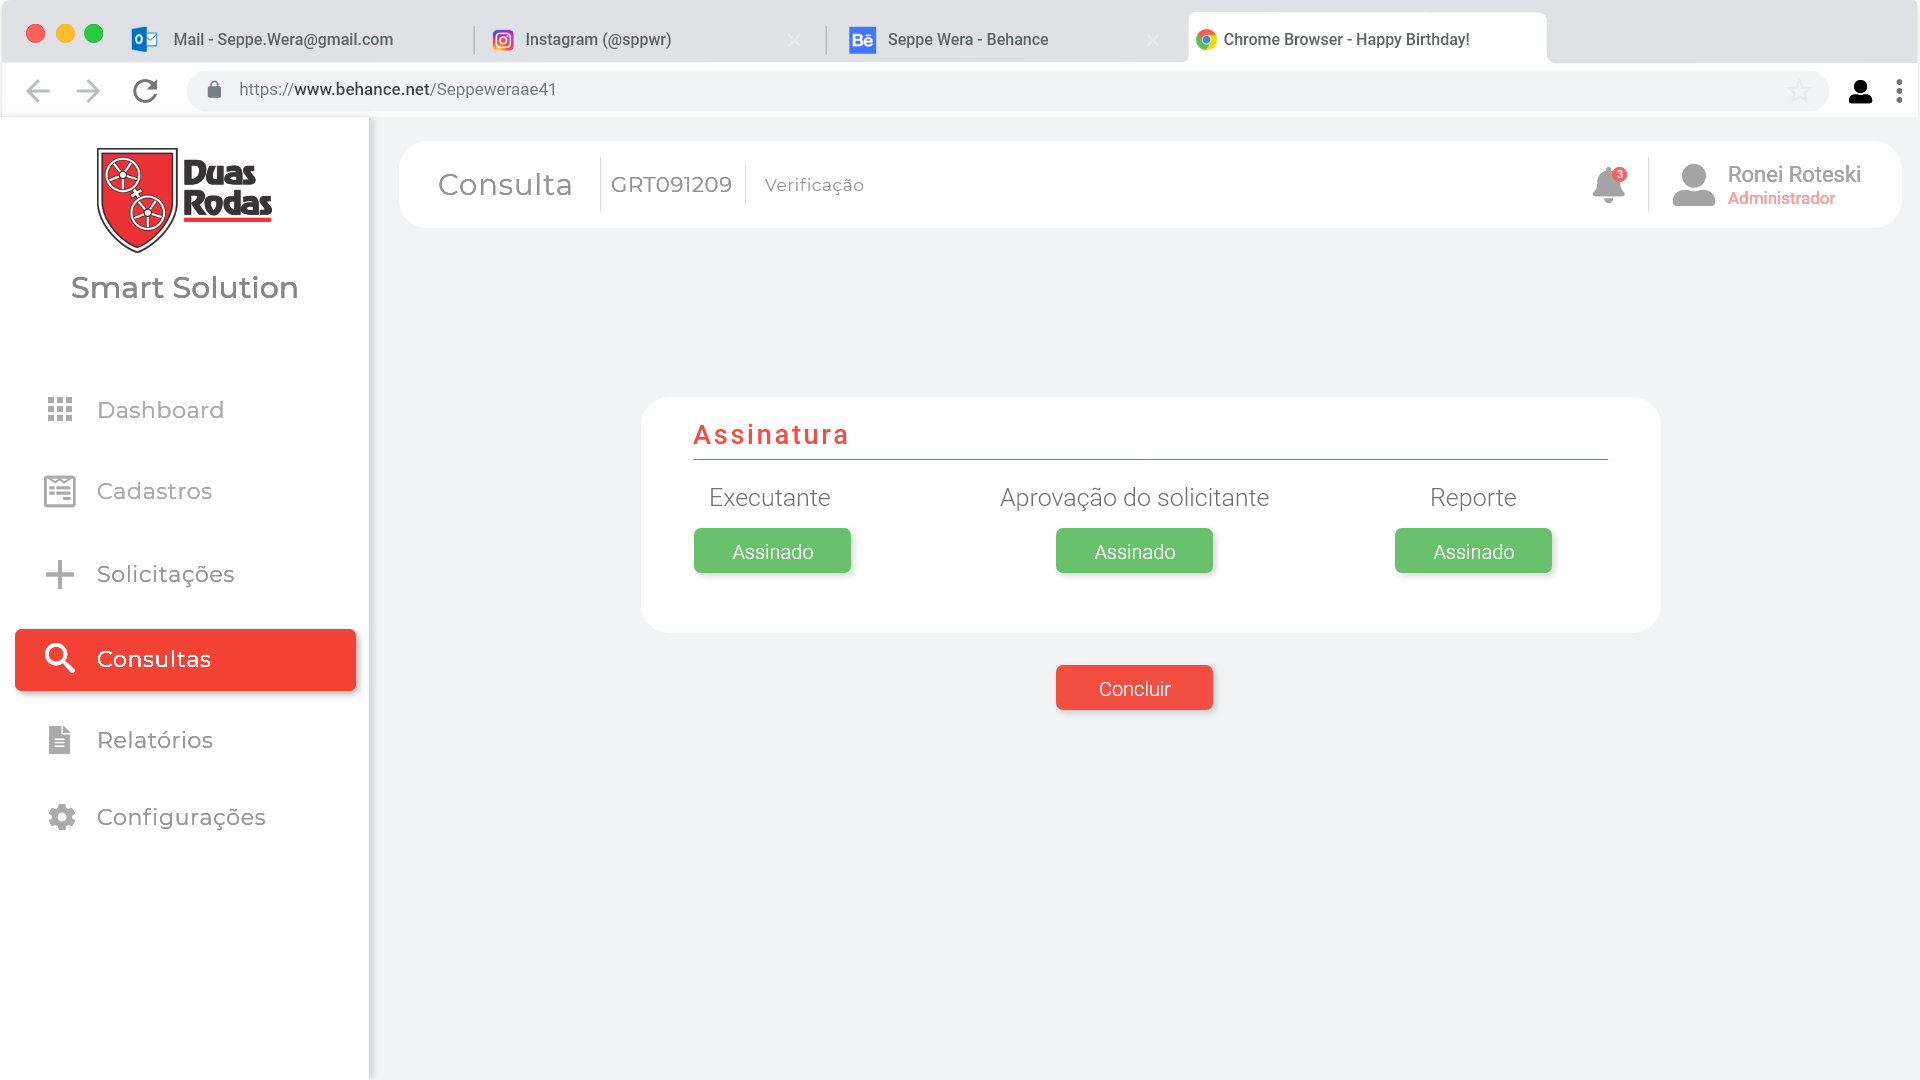
\includegraphics[scale=.32,angle=90]{Figuras/Assinatura_web}}\qquad
	}
	
\end{figure}
\newpage

Telas de relatórios parte 1.
\begin{figure}[htb]
	\centering
	\mbox{%
		\subfigure[Tela de relatórios 1]{\label{Relatorios}%
			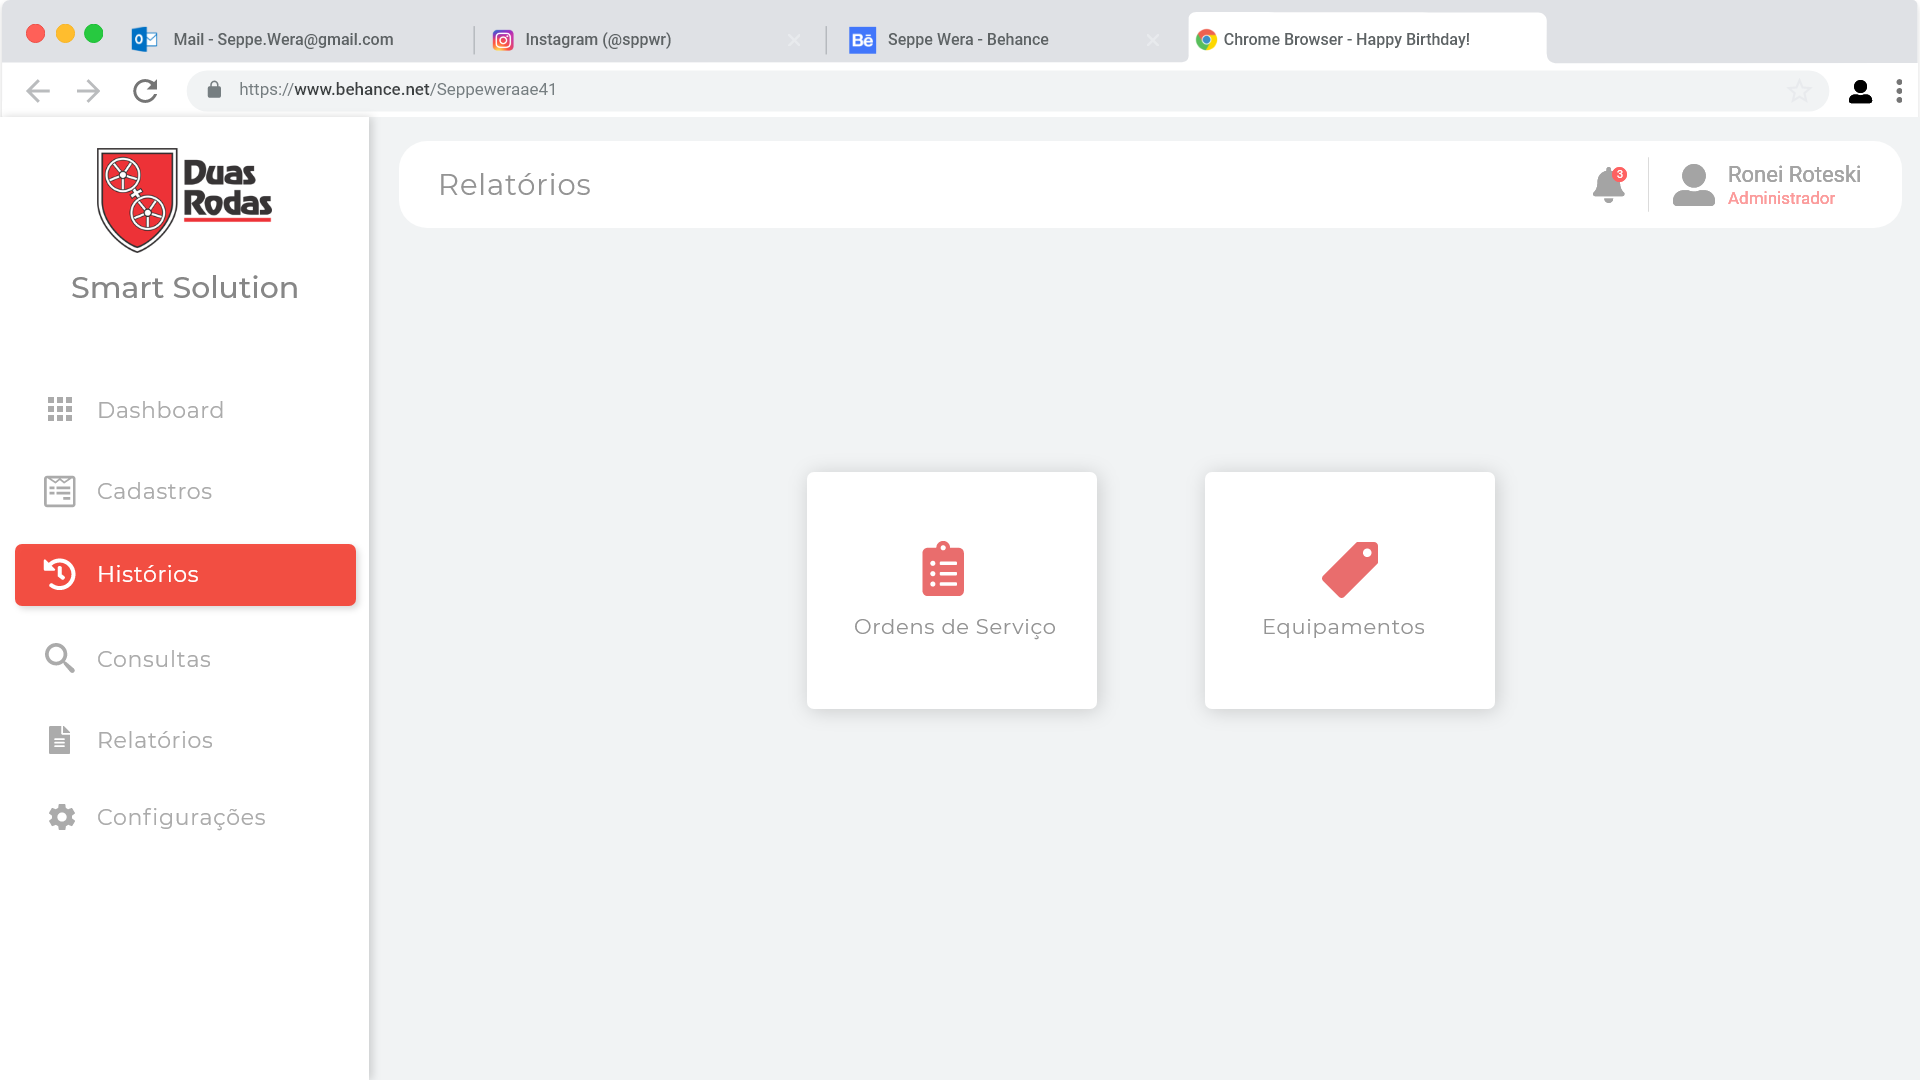
\includegraphics[scale=.32,angle=90]{Figuras/Relatorios}}\qquad
	}
	
\end{figure}
\newpage
Telas de relatórios parte 2.
\begin{figure}[htb]
	\centering
	\mbox{%
		\subfigure[Tela de relatórios 2]{\label{Relatorios_1}%
			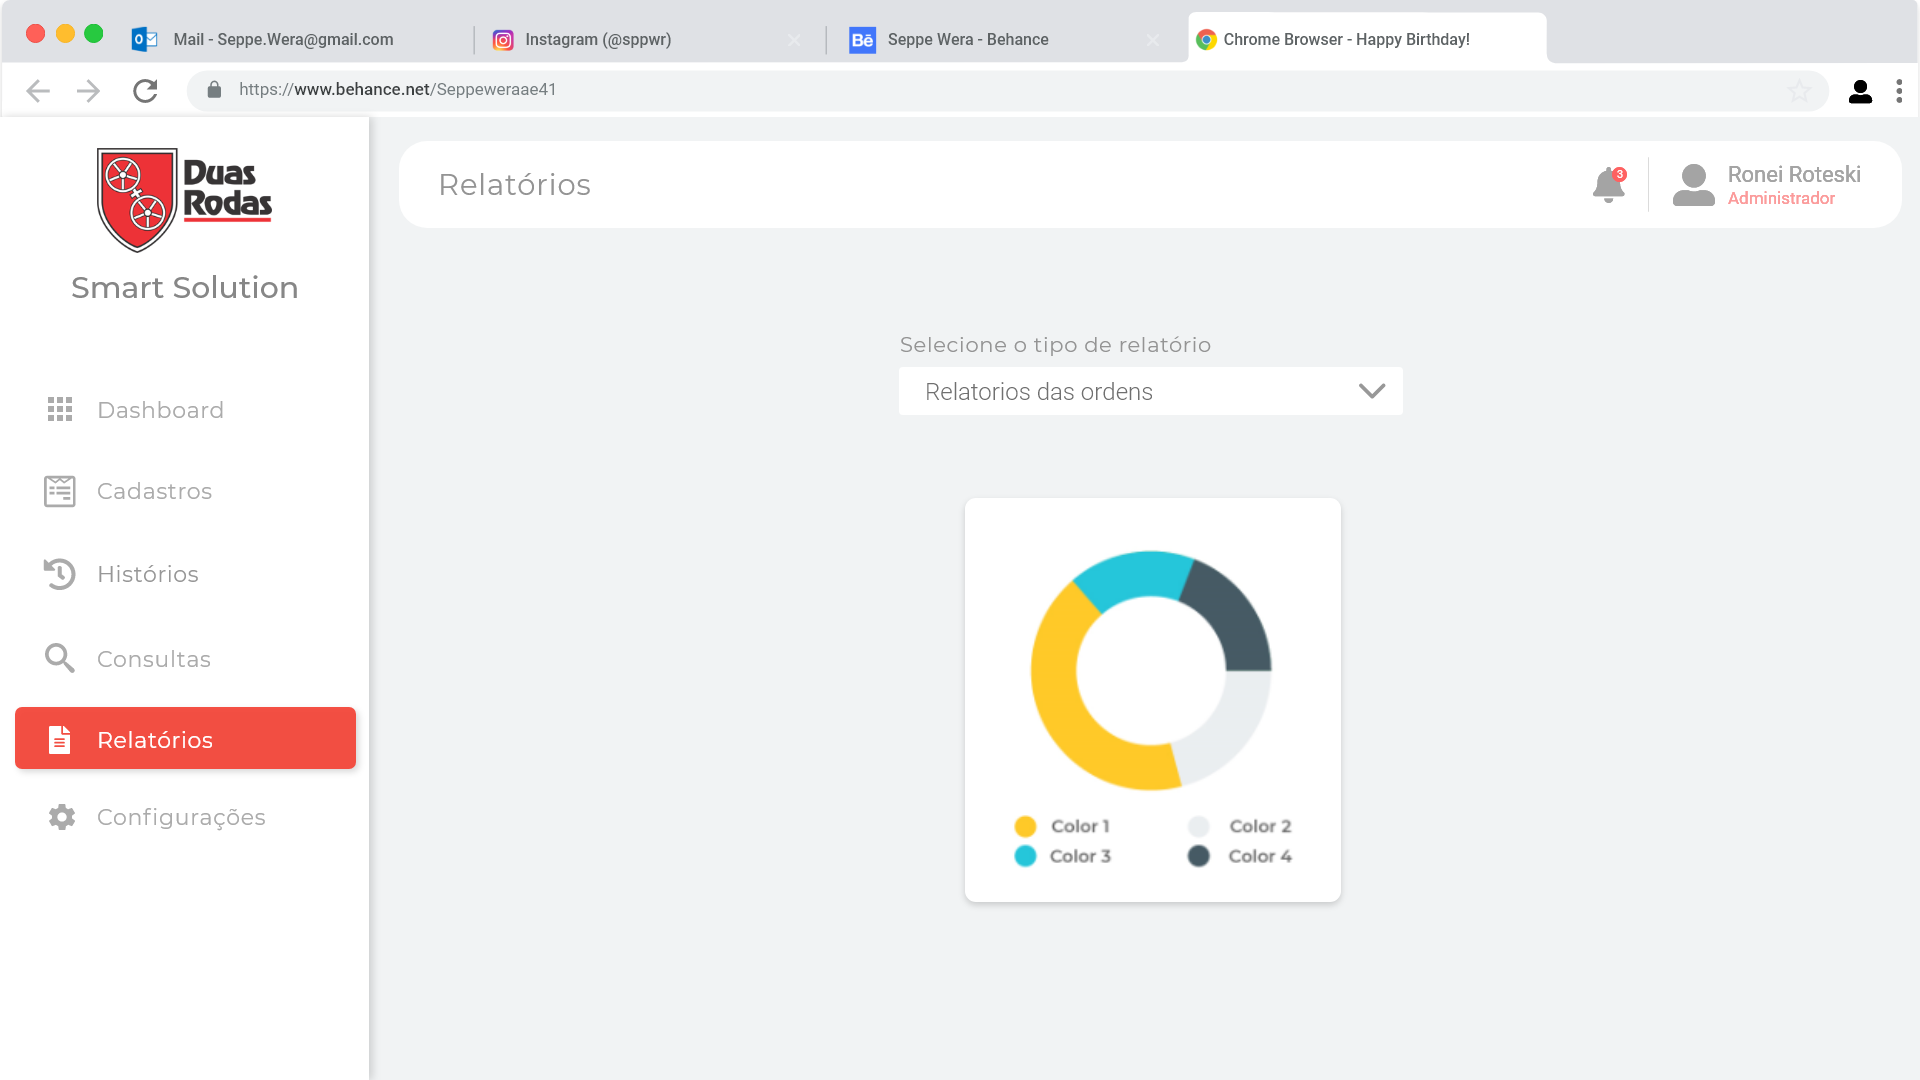
\includegraphics[scale=.32,angle=90]{Figuras/Relatorios_1}}\qquad
	}
	
\end{figure}
\newpage
Telas de relatórios mensais parte 1.
\begin{figure}[htb]
	\centering
	\mbox{%
		\subfigure[Tela de relatórios mensais 1]{\label{Relatorios_mensais}%
			\includegraphics[scale=.32,angle=90]{Figuras/Relatorios_mensais}}\qquad
	}
	
\end{figure}
\newpage
Telas de relatórios mensais parte 2.
\begin{figure}[htb]
	\centering
	\mbox{%
		\subfigure[Tela de relatórios mensais 2]{\label{Relatorios_mensais _1}%
			\includegraphics[scale=.32,angle=90]{Figuras/Relatorios_mensais _1}}\qquad
	}
	
\end{figure}
\newpage
Telas de relatórios mensais parte 3.
\begin{figure}[htb]
	\centering
	\mbox{%
		\subfigure[Tela de relatórios mensais 3]{\label{Relatorios_mensais _2}%
			\includegraphics[scale=.32,angle=90]{Figuras/Relatorios_mensais _2}}\qquad
	}
	
\end{figure}
\newpage
Telas de relatórios de equipamentos.
\begin{figure}[htb]
	\centering
	\mbox{%
		\subfigure[Tela de relatórios equipamentos]{\label{Relatorios_por_equipamento}%
			\includegraphics[scale=.32,angle=90]{Figuras/Relatorios_por_equipamento}}\qquad
	}
	
\end{figure}

\newpage
Tela assinatura apos a verificação dos procedimentos realizados realizados pelo funcionário, que contem também a opção assinatura do solicitante da OS.

\begin{figure}[htb]
	\centering
	\mbox{%
		\subfigure[Tela de assinatura]{\label{verificacao_13_1}%
			\includegraphics[scale=.32,angle=90]{Figuras/verificacao_13_1}}\qquad
	}
	
\end{figure}
\newpage
Tela de Checklist dos Equipamento de proteção individual do funcionário.

\begin{figure}[htb]
	\centering
	\mbox{%
		\subfigure[Tela de Checklist EPI]{\label{CHECKLIST_14}%
			\includegraphics[scale=.32,angle=90]{Figuras/CHECKLIST_14}}\qquad
	}
	
\end{figure}
\newpage
Tela para se justificação do motivo por não utilizar algum EPI especifico.

\begin{figure}[htb]
	\centering
	\mbox{%
		\subfigure[Tela justificação não uso EPI]{\label{CHECKLIST_14_1}%
			\includegraphics[scale=.32,angle=90]{Figuras/CHECKLIST_14_1}}\qquad
	}
	
\end{figure}
\newpage
Tela de assinatura dos responsáveis pela manutenção, solicitante e do administrador.

\begin{figure}[htb]
	\centering
	\mbox{%
		\subfigure[Tela com assinatura dos  responsáveis]{\label{ASSINATURA_15}%
			\includegraphics[scale=.32,angle=90]{Figuras/ASSINATURA_15}}\qquad
	}
	
\end{figure}
\newpage
Tela para cadastrar usuários novos no sistema.

\begin{figure}[htb]
	\centering
	\mbox{%
		\subfigure[Tela para cadastrar usuário]{\label{CADASTRAR_USUARIO_16}%
			\includegraphics[scale=.32,angle=90]{Figuras/CADASTRAR_USUARIO_16}}\qquad
	}
	
\end{figure}


\newpage
\chapter{Utilização de Gamificação para o Sistema }
% ---
Nesse capítulo será evidenciado formas que estimulara os usuários a produzir mais e hospedagem para que o Smart Solution seja colocado fora do ambiente de desenvolvimento.
% ---
%\section{Login social}
% ---
%Apreendemos a usar API de terceiros para registrar apenas as informações desejadas em nosso sistema, para que haja maior segurança para nosso cliente.
% ---
\section{Gamificação}
% ---
A gamificação está muito presente em diversos sistemas e plataformas como uma forma de entreter o usuário utilizando mecânicas e dinâmicas de jogos eletrônicos para engajar as pessoas, com esse conceito, inicialmente foi aplicado ao projeto a opção de classificação das ações realizadas em uma ordem de serviço feita, dessa forma o operador ou responsável pode avaliar o trabalho realizado pelo manutentor trazendo assim feedbacks positivos ou negativos, possibilitando um maior controle de qualidade e se necessário discutir melhorias nos processos.

%referencia a gamificação


% ---
%\section{Marketing}
% ---
%Apreendemos marketing em sala de aula para a ter ma visão ampla da concorrência,de como fazer nosso sistema se destacar, segmentar mercado, a estipular preços,marca, logotipo para nosso produto.
% ---
\section{Hospedagem}
% ---
Como forma de hospedagem uma das tecnologias estudas foi a da IBM Cloud que permite um ambiente de implantação seguro e rápido, pois o mesmo é conectado com o GitHub, dessa forma todo o código é gerenciado pela IBM Cloud na medida em que o projeto é lançado, agilizando o processo de implementação e possibilitando as atualizações do sistema de forma ágil e segura.
% ---
\chapter{Implementação }
% ---
%Neste capitulo visara mostrar os métodos e procedimentos utilizados para implementação da solução do problema evidenciado nos capítulos anteriores .
Neste capítulo será aplicado as técnicas, métodos e procedimentos utilizados para implementação da solução dos problemas evidenciados nos capítulos anteriores.
% ---
\subsection{Códigos da Implementação}

{\color{red} adicionar label e melhorar a descrição}

Nesta parte do código acontece a validação de login do usuário, onde o mesmo se encarrega e enviar os dados informados direto para a API valida-los.
\begin{figure}[H]
	\caption{\label{LoginCodigo}Tela com a implementação do Login da \textit{Smart Solution}}
	\centering
	\mbox{%
		{
			\includegraphics[scale=0.50]{Figuras/LoginCodigo}}\qquad
		
	}
	
	
\end{figure}
\newpage

{\color{red} adicionar label  a Figura X}
Após os dados do usuário serem enviados do APP para a API, neste arquivo a requisição é recebida e enviada para a classe que cuidará das validações.
\begin{figure}[H]
	\caption{\label{Rotalogin}Tela de implementação da rota de Login da\textit{Smart Solution}}
	\centering
	\mbox{%
		{
			\includegraphics[scale=0.50]{Figuras/Rotalogin}}\qquad
		
	}
	
	
\end{figure}
\newpage
{\color{red} adicionar label  a Figura X}

Chegando na classe de validação, os dados que foram enviados da tela de login são validados, se existe algo na requisição, se os dados enviados existem, caso alguma dessas validações venha a ter erros, API rejeita os dados enviados mandando uma mensagem de erro de volta para o usuário. 

\begin{figure}[H]
	\caption{\label{Validacaologin}Tela com a implementação da validação dos dados de Login da\textit{Smart Solution}}
	\centering
	\mbox{%
		{
			\includegraphics[scale=0.50]{Figuras/Validacaologin}}\qquad
		
	}
	
	
\end{figure}
\newpage
{\color{red} adicionar label  a Figura X}

Por fim, depois de os dados terem sido validados, o mesmo será enviado para a classe que é responsável por se comunicar com o banco de dados, buscando esse usuário no banco de dados, casa a busca retorne um erro é porque esse usuário não existe no banco de dados, caso contrário, o sistema retornará a requisição com o status de sucesso, permitindo assim a entrada do usuário no sistema.
\begin{figure}[H]
	\caption{\label{DaoLogin}Tela da implementação com a comunicação para o banco de dados da\textit{Smart Solution}}
	\centering
	\mbox{%
		{
			\includegraphics[scale=0.50]{Figuras/DaoLogin}}\qquad
		
	}
	
	
\end{figure}

\section{Desenvolvimento da Aplicação Cliente}
% ---
{\color{red} adicionar label  a Figura X}

Na aplicação Mobile foi usado a tecnologia Ionic no qual será usado para desenvolver a versão mobile do \textit{Smart Solution}, por ser uma plataforma de desenvolvimento híbrido, possibilitará ser usado tanto no ambiente Android quanto no IOS. Já a aplicação Web será desenvolvida nos próximos semestres e será usado a tecnologia angular por ser semelhante ao Ionic e confiável no desenvolvimento.
% ---

\section{Desenvolvimento da Aplicação Server}
% ---
Para desenvolver a aplicação server, que é responsável pelos endpoints e comunicação com o banco de dados foi utilizado o superconjunto Node.Js, pois essa linguagem facilitará todas as requisições a serem realizadas com dinamismo e agilidade.
% ---
\section{Framework para Conexão Restful}
% ---
A ferramenta para conexão Rest aplicada em conjunto com o Node.Js tanto na API quanto no Client (termo utilizado para definir a versão que o usuário terá interação) possibilita que a comunicação seja feita entre o Client e API e da API para o banco de dados.
% ---
\section{Conexão com Banco de Dados}
% ---
O sistema de gerenciamento banco de dados utilizados foi o MySQL, implementado inicialmente apenas para ambiente de desenvolvimento e teste, permitindo que as vertentes do projeto sejam exploradas de forma livre.
% ---
\newpage
\section{Telas Implementadas}
% ----

{\color{red} adicionar label  as Figuras X e melhorar a introdução}


Tela que permite o usuário entrar no sistema WEB com seu numero de crachá e senha.

\begin{figure}[H]
	\caption{\label{Login_WEB_1}Próprio autor}
	\centering
	\mbox{%
		\subfigure[Tela de login]{\label{Login_WEB_1}%
			\includegraphics[scale=.62,angle=90]{Figuras/Login_WEB_1}}\qquad
		
	}
	
\end{figure}
\newpage

Tela com as opções de cadastramentos disponíveis no sistema.

\begin{figure}[H]
		\caption{\label{Cadastros_Sistema_1}Próprio autor}
	\centering
	\mbox{%
		\subfigure[Tela de opções de cadastros]{\label{Cadastros_Sistema_1}%
			\includegraphics[scale=.50,angle=90]{Figuras/Cadastros_Sistema_1}}\qquad
	}
	
\end{figure}
\newpage

Tela para se cadastrar ordem de serviços no conceito de  step by step no sistema de forma manual primeira etapa.

\begin{figure}[H]
		\caption{\label{step_1}Próprio autor}
	\centering
	\mbox{%
		\subfigure[Tela de cadastro de OS]{\label{step_1}%
			\includegraphics[scale=.42,angle=90]{Figuras/step_1}}\qquad
	}
	
\end{figure}
\newpage

Tela para se cadastrar ordem de serviços no conceito de  step by step no sistema de forma manual segunda etapa

\begin{figure}[H]
		\caption{\label{step_2}Próprio autor}
	\centering
	\mbox{%
		\subfigure[Tela de cadastro de OS]{\label{step_2}%
			\includegraphics[scale=.42,angle=90]{Figuras/step_2}}\qquad
	}
	
\end{figure}
\newpage

Tela para se cadastrar ordem de serviços no conceito de  step by step no sistema de forma manual terceira etapa

\begin{figure}[H]
		\caption{\label{step_3}Próprio autor}
	\centering
	\mbox{%
		\subfigure[Tela de cadastro de OS]{\label{step_3}%
			\includegraphics[scale=.42,angle=90]{Figuras/step_3}}\qquad
	}
	
\end{figure}
\newpage

Tela para cadastrar equipamentos no sistema.

\begin{figure}[H]
		\caption{\label{Cadastro_Equipamento_Sistema}Próprio autor}
	\centering
	\mbox{%
		\subfigure[Tela de cadastrar equipamentos]{\label{Cadastro_Equipamento_Sistema}%
			\includegraphics[scale=.62,angle=90]{Figuras/Cadastro_Equipamento_Sistema}}\qquad
	}
	
\end{figure}
\newpage

Tela para cadastrar componentes de cada maquina.

\begin{figure}[H]
		\caption{\label{Cadastro_Componentes}Próprio autor}
	\centering
	\mbox{%
		\subfigure[Tela de cadastrar componentes]{\label{Cadastro_Componentes}%
			\includegraphics[scale=.62,angle=90]{Figuras/Cadastro_Componentes}}\qquad
	}
	
\end{figure}
\newpage

Tela com finalidade de cadastrar EPI.

\begin{figure}[H]
		\caption{\label{Cadastro_Epi_Sistema}Próprio autor}
	\centering
	\mbox{%
		\subfigure[Tela de cadastrar EPI]{\label{Cadastro_Epi_Sistema}%
			\includegraphics[scale=.62,angle=90]{Figuras/Cadastro_Epi_Sistema}}\qquad
	}
	
\end{figure}
\newpage

Tela para cadastrar causas que ja ocorrerão ou novos.

\begin{figure}[H]
		\caption{\label{Cadastro_Causa_Defeito}Próprio autor}
	\centering
	\mbox{%
		\subfigure[Tela de cadastrar causas]{\label{Cadastro_Causa_Defeito}%
			\includegraphics[scale=.62,angle=90]{Figuras/Cadastro_Causa_Defeito}}\qquad
	}
	
\end{figure}
\newpage

Tela para cadastrar sintomas que ja ocorrerão ou novos.

\begin{figure}[H]
		\caption{\label{Cadastro_Sintomas}Próprio autor}
	\centering
	\mbox{%
		\subfigure[Tela de cadastrar sintomas]{\label{Cadastro_Sintomas}%
			\includegraphics[scale=.62,angle=90]{Figuras/Cadastro_Sintomas}}\qquad
	}
	
\end{figure}
\newpage

Tela para cadastrar localização do equipamento.

\begin{figure}[H]
		\caption{\label{Cadastro_Localizaçao}Próprio autor}
	\centering
	\mbox{%
		\subfigure[Tela de cadastrar localização do equipamento]{\label{Cadastro_Localizaçao}%
			\includegraphics[scale=.62,angle=90]{Figuras/Cadastro_Localizaçao}}\qquad
	}
	
\end{figure}
\newpage


Tela de cadastro de centro de trabalho.

\begin{figure}[H]
		\caption{\label{Cadastro_Centro_Trabalho}Próprio autor}
	\centering
	\mbox{%
		\subfigure[Tela de cadastrar centro de trabalho]{\label{Cadastro_Centro_Trabalho}%
			\includegraphics[scale=.62,angle=90]{Figuras/Cadastro_Centro_Trabalho}}\qquad
	}
	
\end{figure}
\newpage

Tela para cadastrar tipo de ordem serviço.

\begin{figure}[H]
		\caption{\label{Cadastro_Tipo_Ordem}Próprio autor}
	\centering
	\mbox{%
		\subfigure[Tela de cadastrar tipo de ordem serviço]{\label{Cadastro_Tipo_Ordem}%
			\includegraphics[scale=.62,angle=90]{Figuras/Cadastro_Tipo_Ordem}}\qquad
	}
	
\end{figure}
\newpage


Tela com as opções de cadastrar e listar usuários no sistema.

\begin{figure}[H]
		\caption{\label{listagem_e_cadastro_de_usuario}Próprio autor}
	\centering
	\mbox{%
		\subfigure[Tela de cadastrar e listar usuários]{\label{listagem_e_cadastro_de_usuario}%
			\includegraphics[scale=.47,angle=90]{Figuras/listagem_e_cadastro_de_usuario}}\qquad
	}
	
\end{figure}
\newpage

Tela com as opções de consulta de ordens de serviço no sistema, podendo ser por numero da ordem ou algum dos filtros disponíveis ao usuário.

\begin{figure}[H]
		\caption{\label{Consulta_ordem}Próprio autor}
	\centering
	\mbox{%
		\subfigure[Tela de cadastrar e listar usuários]{\label{Consulta_ordem}%
			\includegraphics[scale=.45,angle=90]{Figuras/Consulta_ordem}}\qquad
	}
	
\end{figure}
\newpage
% ------
%\chapter{Implantação }
\chapter{Conclusões e Trabalhos Futuros}
%\section{Implementação}
Com o desenvolvimento do projeto Smart Solution pode-se perceber a importância de um sistema WEB e Mobile para o mercado industrial. Para tal fato, o projeto em questão teve inicialmente como foco principal o desenvolvimento da parte mobile, onde foi implementado sua interface, aplicado as regras de negócio e concluída a API de conexão com o banco de dados. Sendo assim o projeto integrador encontra-se parcialmente funcional, podendo sofrer melhorias no decorrer de todo o processo de desenvolvimento.

Para as próximas etapas será melhorado o sistema de segurança da aplicação com novas implementações e adaptações, melhorando suas funcionalidades. Também será desenvolvimento a aplicação WEB visando a melhoria do gerenciamento das ordens de serviço e a possibilidade de novos cadastros caso haja impossibilidades de comunicação com o SAP.

Para finalizar os diferenciais do Smart Solution para soluções já implementadas, foi proposta a inclusão de um módulo de controle de estoque. Este módulo permite que haja um gerenciamento do estoque do almoxarifado e consequentemente facilitando as solicitações de novos equipamentos ou peças.

Sendo assim, dentre as soluções propostas, o Smart Solution será o sistema que melhor se adaptará as necessidades da empresa Duas Rodas, contando com a versão Mobile e WEB proporcionando maior liberdade aos colaboradores.


%Para as próximas etapas de desenvolvimento será melhorado o sistema de segurança da aplicação mobile entre outras pequenas melhorias e novas implementações de funcionalidades. Será desenvolvido a aplicação WEB com foco no gerenciamento das ordens, possibilidade de cadastro caso algo impossibilite a comunicação entre o \textit{Smart Solution} e o SAP. Analises das ordens de serviços também é uma realidade para as futuras implementações. Outro ponto importante é o sistema de estoque em conjunto com o Smart Solution para gerenciar o estoque do almoxarifado e solicitações de novos equipamentos ou peças.







%\include{cap10}
% ---
% Finaliza a parte no bookmark do PDF, para que se inicie o bookmark na raiz
% ---
\bookmarksetup{startatroot}% 
% ---

% ----------------------------------------------------------
% ELEMENTOS PÓS-TEXTUAIS
% ----------------------------------------------------------
\postextual


% ----------------------------------------------------------
% Referências bibliográficas
% ----------------------------------------------------------

\bibliography{refereces}
% ----------------------------------------------------------
% Glossário
% ----------------------------------------------------------
%
% Consulte o manual da classe abntex2 para orientações sobre o glossário.
%
%\glossary

% ----------------------------------------------------------
% Apêndices
% ----------------------------------------------------------
%\begin{apendicesenv}

% Imprime uma página indicando o início dos apêndices
%\partapendices



%\end{apendicesenv}

% ----------------------------------------------------------
% Anexos

% ----------------------------------------------------------
%\begin{anexosenv}

% Imprime uma página indicando o início dos anexos
%\partanexos

%\include{anexo}

%\end{anexosenv}

%---------------------------------------------------------------------
% INDICE REMISSIVO
%---------------------------------------------------------------------

%\printindex

\end{document}
% FIM